% % % % % % % % % % % % % % % % % % % % % % % % % % % % % % % % % % % % % % % % %
% "THE BEER-WARE LICENSE" (Revision 42, Hannes Badertscher):
% Reto Christen (reto.christen@hsr.ch) and Thomas Franz (thomas.franz@hsr.ch) 
% wrote this file. As long as you retain this notice you can do whatever you want 
% with this stuff. If we meet some day, and you think this stuff is worth it, 
% you can buy us a beer in return. 
% - Reto Christen & Thomas Franz
% % % % % % % % % % % % % % % % % % % % % % % % % % % % % % % % % % % % % % % % %

% Dokumentinformationen
\title{Applied Electromagnetics}
\author{HSR-Stud R. Christen, Th. Franz}
%\version{$Revision: Marie $ - powered by \LaTeX}
\documentclass[8spt,twoside,a4paper,fleqn]{article}

% Header
%%%%%%%%%%%%%%%%%%%%%%%%%%%%%%%%%%%%%%%
%% Makros & anderer Low-Level bastel %%
%%%%%%%%%%%%%%%%%%%%%%%%%%%%%%%%%%%%%%%
\makeatletter
%% Makros für Titel, Autor und Datum 
%% Dank diesem Makro stehen Titel, Autor und Datum überall im Dokument zur verfügung
%% Date hat zudem den Default-Wert \today
\def\@Title{}
\def\@Author{}
\def\@Date{\today}
\newcommand{\Title}{\@Title}
\newcommand{\Author}{\@Author}
\newcommand{\Date}{\@Date}
\AtBeginDocument{%
  \let\@Title\@title
  \let\@Author\@author
  \let\@Date\@date
}

%% Makros für den Arraystretch (bei uns meist in Tabellen genutzt, welche Formeln enthalten)
% Default Value
\def\@ArrayStretchDefault{1} % Entspricht der Voreinstellung von Latex

% Setzt einen neuen Wert für den arraystretch
\newcommand{\setArrayStretch}[1]{\renewcommand{\arraystretch}{#1}}

% Setzt den arraystretch zurück auf den default wert
\newcommand{\resetArrayStretch}{\renewcommand{\arraystretch}{\@ArrayStretchDefault}}

% Makro zum setzten des Default arraystretch. Kann nur in der Präambel verwendet werden.
\newcommand{\setDefaultArrayStretch}[1]{%
	\AtBeginDocument{%
		\def\@ArrayStretchDefault{#1}
		\renewcommand{\arraystretch}{#1}
	}
}
\makeatother


%%%%%%%%%%%%%%%%%%%%%%%
%% Wichtige Packages %%
%%%%%%%%%%%%%%%%%%%%%%%
\usepackage[utf8]{inputenc} % UTF-8 unterstützung
\usepackage[english, ngerman]{babel} % Silbentrennung
\usepackage[automark]{scrpage2} % Header und Footer
\usepackage{tabularx}

% Für Abbildungen mit mehreren kleinen Bilder
% Doku: http://www.ctan.org/tex-archive/macros/latex/contrib/caption/
\usepackage{caption}
\usepackage{subcaption}

\ifx \GUARDhsrColors \undefined
\def\GUARDhsrColors{}

\usepackage[table]{xcolor}

\definecolor{HSRWhite}{cmyk}{0,0,0,0}

\definecolor{HSRBlue}{cmyk}{1,0.4,0,0.2}
\definecolor{HSRBlue80}{cmyk}{0.8,0.32,0,0.16}
\definecolor{HSRBlue60}{cmyk}{0.6,0.24,0,0.12}
\definecolor{HSRBlue40}{cmyk}{0.4,0.16,0,0.08}
\definecolor{HSRBlue20}{cmyk}{0.2,0.08,0,0.04}

\definecolor{HSRLightGray}{cmyk}{0,0,0,0.30}
\definecolor{HSRLightGray80}{cmyk}{0,0,0,0.24}
\definecolor{HSRLightGray60}{cmyk}{0,0,0,0.18}
\definecolor{HSRLightGray40}{cmyk}{0,0,0,0.12}
\definecolor{HSRLightGray20}{cmyk}{0,0,0,0.06}

\definecolor{HSRSchwarz}{cmyk}{0,0,0,1}
\definecolor{HSRSchwarz80}{cmyk}{0,0,0,0.8}
\definecolor{HSRSchwarz60}{cmyk}{0,0,0,0.6}
\definecolor{HSRSchwarz40}{cmyk}{0,0,0,0.4}
\definecolor{HSRSchwarz20}{cmyk}{0,0,0,0.2}

\definecolor{HSRHematite}{cmyk}{0.6,1,0.4,0.2}
\definecolor{HSRHematite80}{cmyk}{0.48,0.80,0.32,0.16}
\definecolor{HSRHematite60}{cmyk}{0.36,0.60,0.24,0.12}
\definecolor{HSRHematite40}{cmyk}{0.24,0.40,0.16,0.08}
\definecolor{HSRHematite20}{cmyk}{0.12,0.20,0.08,0.04}

\definecolor{HSRLakeGreen}{cmyk}{0.70,0.30,0.45,0.05}
\definecolor{HSRLakeGreen80}{cmyk}{0.56,0.24,0.36,0.03}
\definecolor{HSRLakeGreen60}{cmyk}{0.42,0.18,0.27,0.02}
\definecolor{HSRLakeGreen40}{cmyk}{0.28,0.06,0.13,0.06}
\definecolor{HSRLakeGreen20}{cmyk}{0.14,0.06,0.09,0.01}

\definecolor{HSRReed}{cmyk}{0.10,0.25,0.45,0.60}
\definecolor{HSRReed80}{cmyk}{0.08,0.20,0.36,0.48}
\definecolor{HSRReed60}{cmyk}{0.06,0.15,0.27,0.36}
\definecolor{HSRReed40}{cmyk}{0.04,0.10,0.18,0.24}
\definecolor{HSRReed20}{cmyk}{0.02,0.05,0.09,0.12}

\definecolor{HSRPetrol}{cmyk}{1,0.18,0,0.45}
\definecolor{HSRPetrol80}{cmyk}{0.64,0.08,0.12,0.32}
\definecolor{HSRPetrol60}{cmyk}{0.48,0.06,0.09,0.24}
\definecolor{HSRPetrol40}{cmyk}{0.32,0.04,0.06,0.16}
\definecolor{HSRPetrol20}{cmyk}{0.16,0.02,0.03,0.08}

\definecolor{HSRBasswood}{cmyk}{0.25,0.05,0.70,0.15}
\definecolor{HSRBasswood80}{cmyk}{0.20,0.04,0.56,0.12}
\definecolor{HSRBasswood60}{cmyk}{0.15,0.03,0.42,0.09}
\definecolor{HSRBasswood40}{cmyk}{0.10,0.02,0.28,0.06}
\definecolor{HSRBasswood20}{cmyk}{0.05,0.01,0.14,0.03}


\fi
\ifx\GUARDmathe\undefined
\def\GUARDmathe{}

\usepackage{amssymb}
% Das mathtools package ist eine Erweiterung zum amsmath package.
% Das amsmath package wird dabei automatisch geladen
\usepackage{mathtools}


% Package mit vielen weiteren Mathe Symbolen
% http://www.ctan.org/tex-archive/fonts/mathabx
\usepackage{mathabx}

% This package defines commands to access bold math symbols. The basic command
% is \bm which may be used to make the math expression in its argument be typeset
% using bold fonts.
\usepackage{bm}

\fi
\ifx\GUARDenumitem\undefined
\def\GUARDenumitem{}

\usepackage{enumitem}

\fi

% Seitenränder für Formelsammlungen
\usepackage[left=1cm,right=1cm,top=1cm,bottom=1cm,includeheadfoot]{geometry}

\usepackage{multirow} % Create tabular cells spanning multiple rows
\usepackage{multicol} % In­ter­mix sin­gle and mul­ti­ple columns
\usepackage{rotating} % Rotation tools, including rotated fullpage floats


%%%%%%%%%%%%%%%%%%%%%%%%%%%%%%%%%%%
%% Layout der Kopf und Fusszeile %%
%%%%%%%%%%%%%%%%%%%%%%%%%%%%%%%%%%%
\deftripstyle{zusammenfassung}[0pt][0.5pt]
	{\Title}	% Kopfzeile innen
	{\headmark}	% Kopfzeile mitte
	{\pagemark}	% Kopfzeile aussen
	{\Author}	% Fusszeile innen
	{
\includegraphics[width=1.6cm]{./header/lizenzen/cc-by-nc-sa/small.png}}			% Fusszeile mitte
	{\Date}	% Fusszeile aussen
\pagestyle{zusammenfassung}



% Makros für Verweise auf ein Buch oder Skript
\newcommand{\buch}[1]{\texorpdfstring{$_{\textcolor{HSRLakeGreen}{\mbox{\small{#1}}}}$}{}}
\newcommand{\buchSeite}[1]{\texorpdfstring{\ensuremath{_{\textcolor{red}{\mbox{\small{ S#1}}}}}}{}}
\newcommand{\skript}[1]{\texorpdfstring{$_{\textcolor{HSRReed}{\mbox{\small{#1}}}}$}{}}
\newcommand{\formelbuch}[1]{$_{\textcolor{red}{\mbox{\small{S#1}}}}$}

% Zeilenhöhe Tabellen:
\newcommand{\arraystretchOriginal}{1.5}
\renewcommand{\arraystretch}{\arraystretchOriginal}

\setlength{\parindent}{0pt}
\usepackage{tikz}
\usepackage{textcomp, pxfonts, enumitem}
\usetikzlibrary{intersections}
\usepackage{longtable}
\usetikzlibrary{calc}
\usetikzlibrary{through}

\usepackage{adjustbox}
\usepackage{caption}
\usepackage{graphicx}
\usepackage{subcaption}
% Setzt ein zentriertes Bild mit Beschriftung
% Syntax: \abb{Pfad zum Bild}{Bildgrösse}{Beschriftung des Bildes}
\newcounter{abbildungen} \stepcounter{abbildungen}
\newcommand{\abb}[3]{
\begin{center}
\includegraphics[width=#2]{#1} \\
Abbildung \arabic{abbildungen}: #3
\stepcounter{abbildungen}
    \end{center}
}

% Document
\begin{document}
\section{Fundamentals}

\begin{tabular}{|l|c|c|}
\hline \textbf{Description} & \textbf{Symbol} & \textbf{Unit} \\ 
\hline Free electric charge in the system & $Q$ & $C = As$ \\
\hline Volumetric free charge density & $\rho$ & $\frac{C}{m^3}$ \\
\hline Individual electric current flowing through the surface $S$ & $I_i$ & $A$ \\
\hline Magnetic flux through the surface $S$ & $\Phi$	& $Wb = Tm^2$\\
\hline Induced voltage along the closed loop $\delta S$ & $u_i$ & $V$ \\
\hline Electric current density & $\vec{J} = \sigma \vec{E}$ & $\frac{A}{m^2}$\\
\hline Electric flux density & $\vec{D} = \varepsilon \vec{E}$ & $\frac{C}{m^2} = \frac{As}{m^2}$\\
\hline Electric field & $\vec{E} = \frac{\vec{D}}{\varepsilon}$ & $\frac{V}{m}$\\
\hline Magnetic flux density & $\vec{B} = \mu \vec{H}$ & $T = \frac{Vs}{m^2}$\\
\hline Magnetic field & $\vec{H} = \frac{\vec{B}}{\mu}$ & $\frac{A}{m}$\\
\hline Electric permittivity & $\varepsilon = \varepsilon_0 \varepsilon_r$ & $\varepsilon_0 = 8.85 \cdot 10^{-12} \left[\frac{F}{m} = \frac{As}{Vm}\right]$\\
\hline Magnetic permeability & $\mu = \mu_0 \mu_r$ & $\mu_0 = 4\pi \cdot 10^{-7} \left[\frac{Tm}{A} = \frac{H}{m} = \frac{Vs}{Am}\right]$ \\
\hline Specific electric conductivity & $\sigma = \frac{1}{\rho}$ & $\sigma_\textrm{Cu} = 5.96 \cdot 10^7 \left[\frac{S}{m} = \frac{1}{\Omega m}\right]$ \\
\hline Electric potential & $\varphi$ & $V$ \\
\hline Magnetic potential & $A$ & $Tm = \frac{Vs}{m}$ \\
\hline 
\end{tabular} 

\textbf{\\ \\ Gradient\\ \\}
\begin{minipage}[lt]{5cm}
	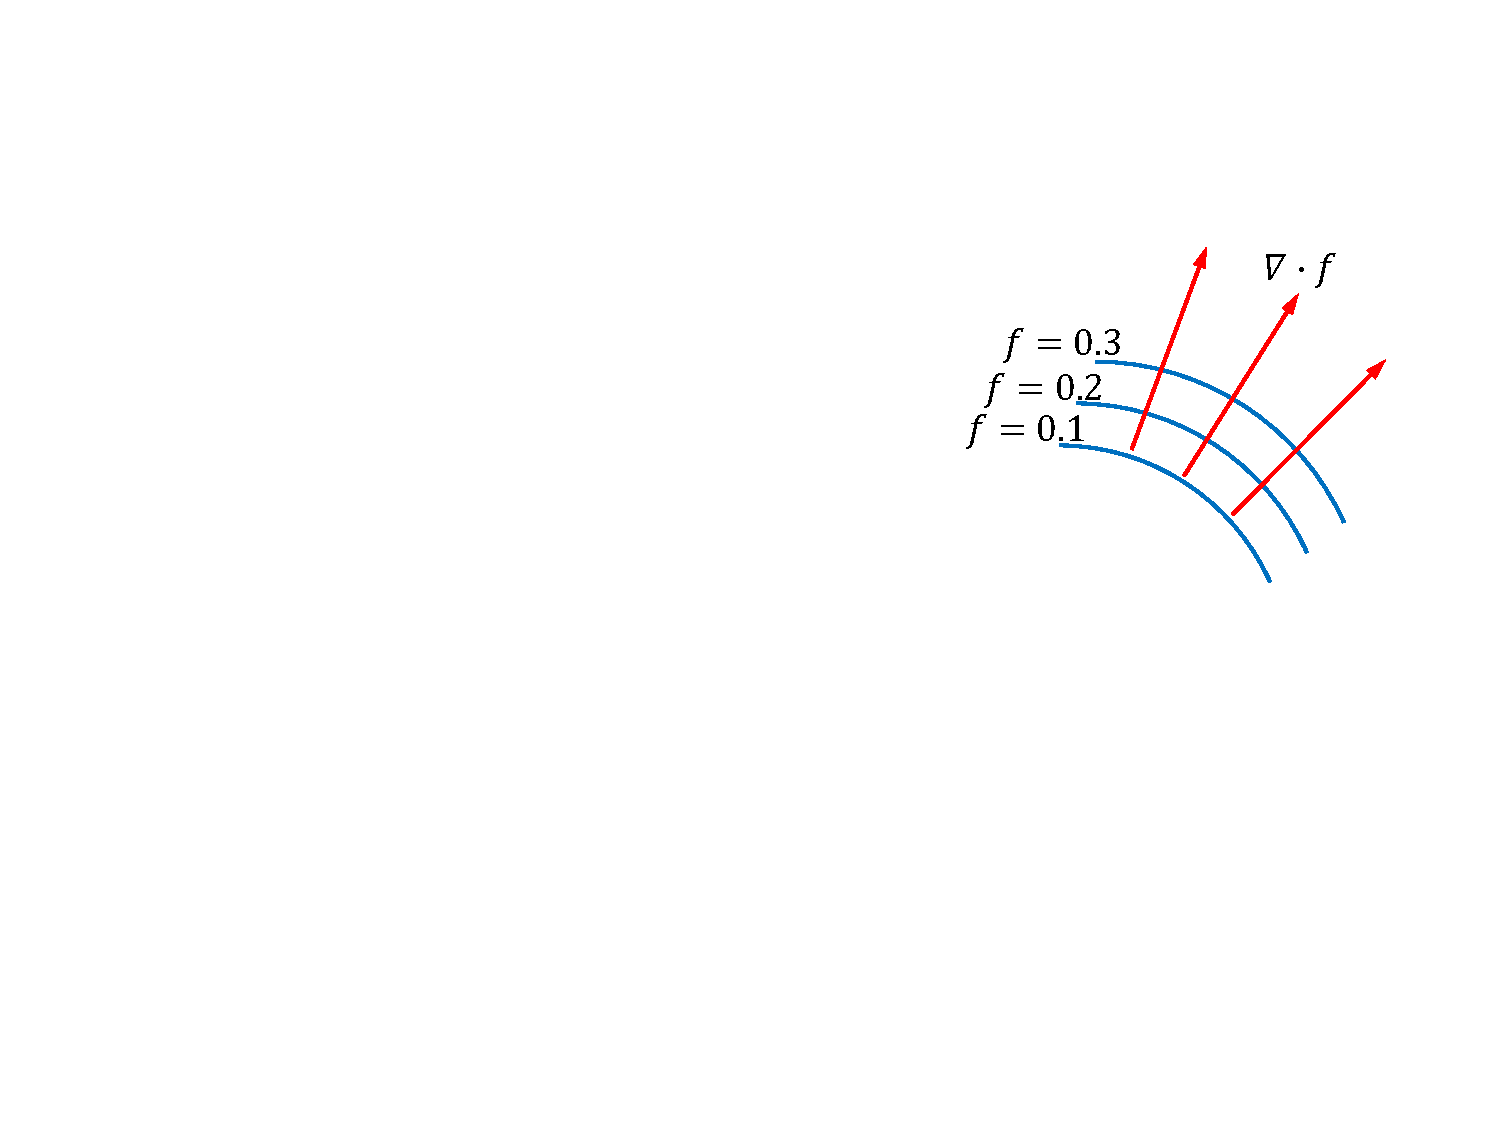
\includegraphics[width=.8\textwidth]{./images/Gradient.pdf}
\end{minipage}
\begin{minipage}[rt]{13cm}
	The gradient of a scalar field reveals the direction of the steepest ascent of the scalar function (perpendicular to the corresponding isolines of the function). \\ \\
	\begin{tabular}{ll}
		Scalar field: & \(\displaystyle f = f\left(\vec{r}\right) = f\left(x,y,z\right) \) \\ 
		Gradient is a vector: & \(\displaystyle \textrm{grad }f = \lim\limits_{\textrm{diameter}\left(D\right)\rightarrow 0} \frac{\oiint_{\textrm{boundary}\left(D\right)}f \cdot \vec{dA}}{\textrm{measure}\left(D\right)}, D\subseteq R^3 \) \\
		Gradient in Cartesian coordinates: & \(\displaystyle \textrm{grad }f = \frac{\partial f}{\partial x} \cdot \vec{e_x}+\frac{\partial f}{\partial y} \cdot \vec{e_y}+\frac{\partial f}{\partial z} \cdot \vec{e_z} \) \\ 
		$\nabla$-operator (Nabla): & \(\displaystyle \nabla = \frac{\partial}{\partial x} \cdot \vec{e_x}+\frac{\partial}{\partial y} \cdot \vec{e_y}+\frac{\partial}{\partial z} \cdot \vec{e_z} \)\\
		Gradient and $\nabla$-operator: & \(\displaystyle \textrm{grad }f = \nabla \cdot f \)\\
	\end{tabular} 
\end{minipage}

\textbf{\\ \\ Divergence\\ \\}
\begin{minipage}[lt]{5cm}
	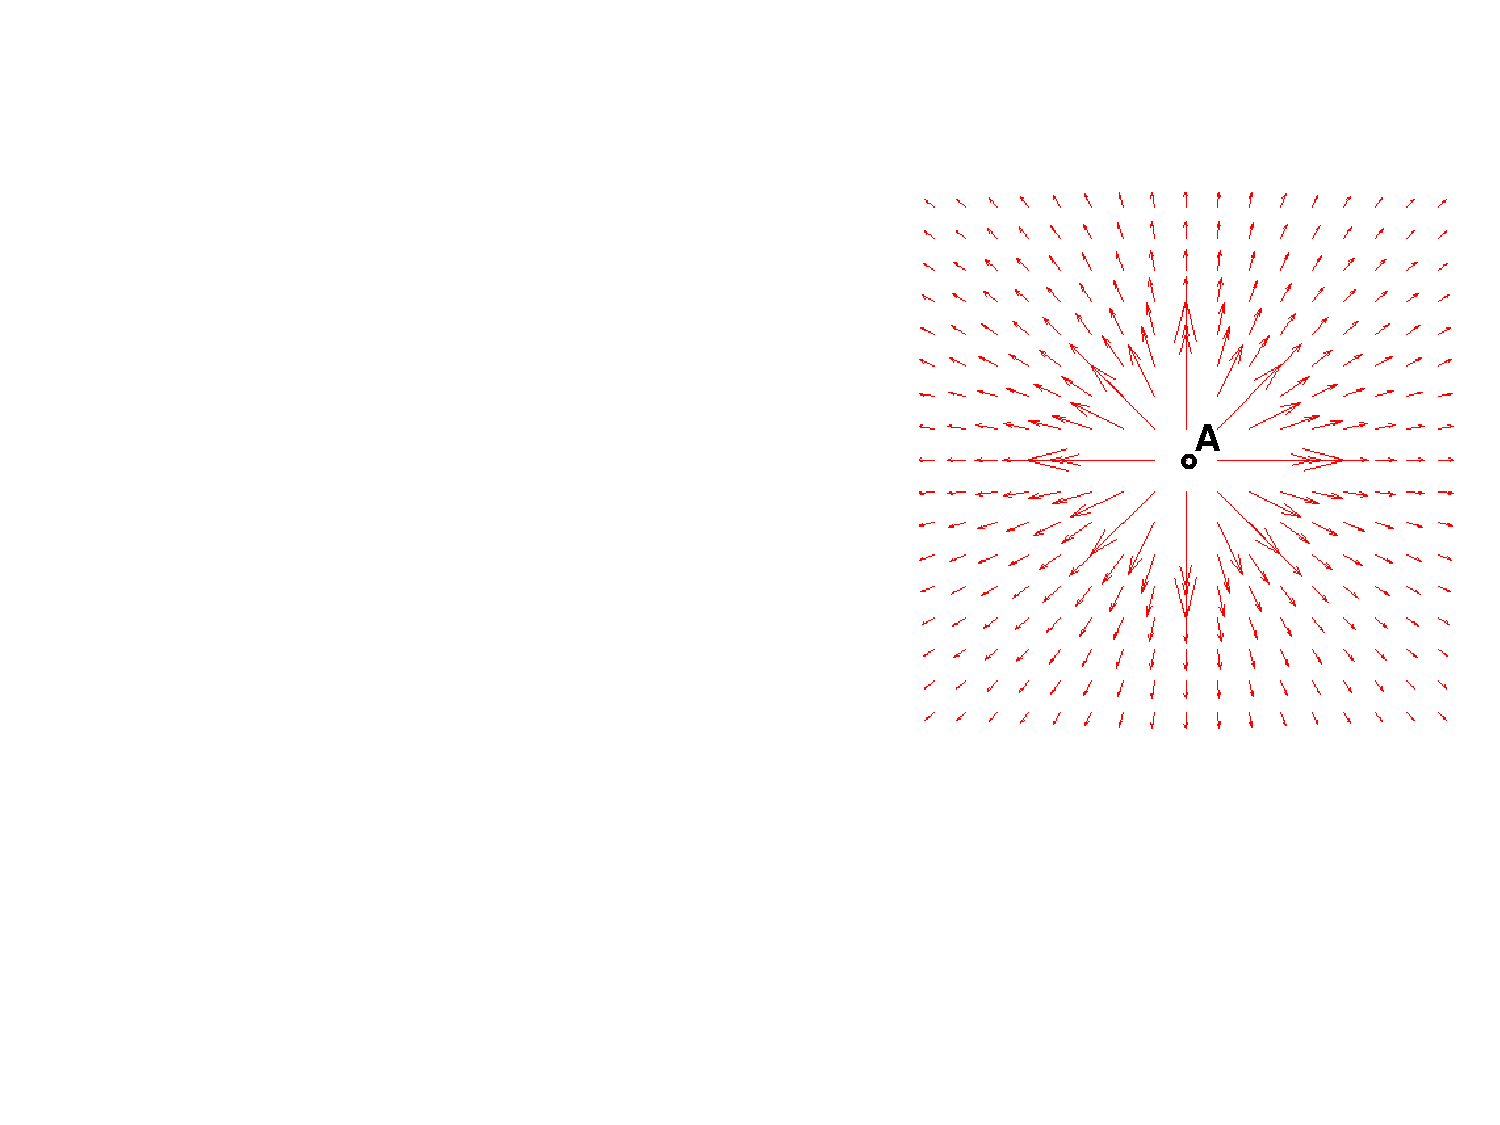
\includegraphics[width=.8\textwidth]{./images/Divergence.pdf}
\end{minipage}
\begin{minipage}[rt]{13cm}
	In the central point $A$ of this field distribution is: $\mathrm{div}~\vec{a} > 0$. Generally speaking, a positive or negative divergence reveals a field source or a field sink, respectively. \\ \\
	\begin{tabular}{ll}
		Vector field: & \(\displaystyle \vec{a} = \vec{a}\left(\vec{r}\right) = \vec{a}\left(x,y,z\right)\) \\
		Divergence is a scalar: & \(\displaystyle \mathrm{div}~\vec{a} = \lim\limits_{\textrm{diameter}\left(D\right)\rightarrow 0} \frac{\oiint_{\textrm{boundary}\left(D\right)} \vec{a} \cdot \vec{dA}}{\textrm{measure}\left(D\right)}, D\subseteq R^3\) \\
		Divergence in Cartesian coordinates: & \(\displaystyle \mathrm{div}~\vec{a} = \frac{\partial a_x}{\partial x} + \frac{\partial a_y}{\partial y} + \frac{\partial a_z}{\partial z} \)\\
		Divergence and $\nabla$-operator: & \(\displaystyle \mathrm{div}~\vec{a} = \nabla \cdot \vec{a} \) \\
	\end{tabular}
\end{minipage}

\textbf{\\ \\ Curl\\ \\}
\begin{minipage}[lt]{5cm}
	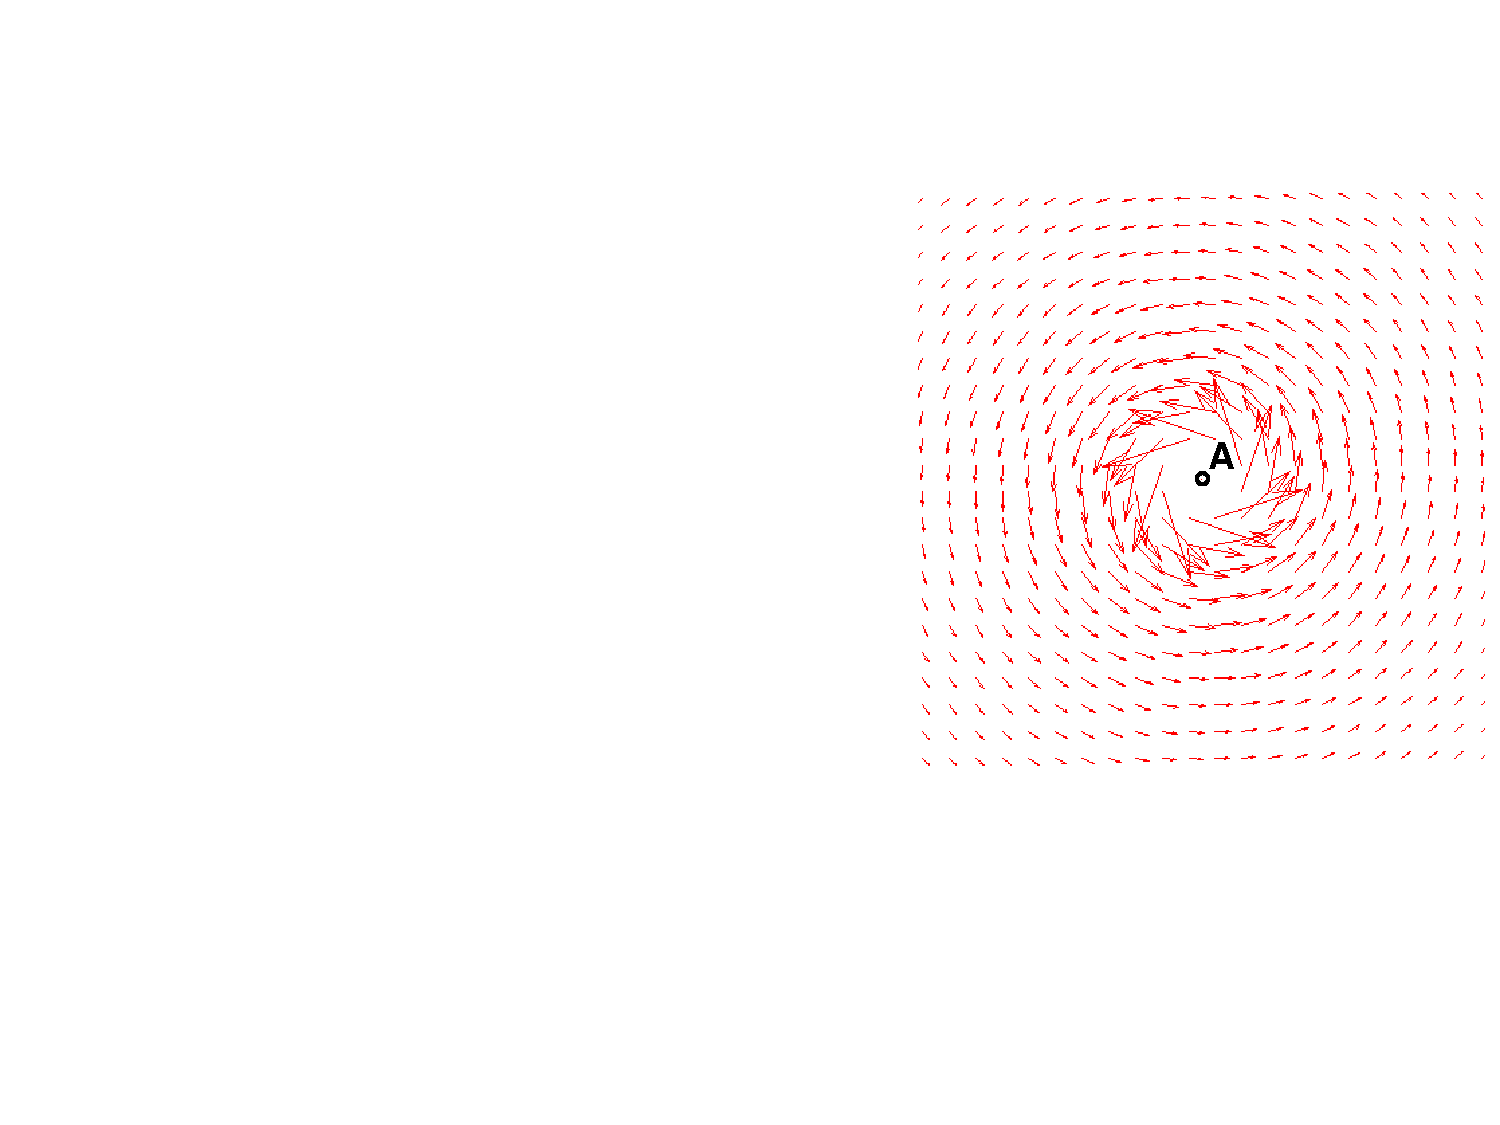
\includegraphics[width=.8\textwidth]{./images/Curl.pdf}
\end{minipage}
\begin{minipage}[rt]{13cm}
	In the central point $A$ of this field distribution is: $\textrm{curl}~\vec{a} > 0$. Generally speaking non-zero curl reveals a rotational field character. (Curl looks what stays in this area).\\ \\
	\begin{tabular}{ll}
		Vector field: & \(\displaystyle \vec{a} = \vec{a}\left(\vec{r}\right) = \vec{a}\left(x,y,z\right)\)\\
		Curl is a vector: & \(\displaystyle \textrm{curl }\vec{a} = \lim\limits_{\textrm{diameter}\left(D\right)\rightarrow 0} \frac{\oiint_{\textrm{boundary}\left(D\right)} \vec{dA} \times \vec{a}}{\textrm{measure}\left(D\right)}, D\subseteq R^3\)\\
		Curl in Cartesian coordinates: & \(\displaystyle \textrm{curl }\vec{a} = 
		\begin{vmatrix}
			\vec{e_x} & \vec{e_y} & \vec{e_z} \\
			\frac{\partial}{\partial x} & \frac{\partial}{\partial y} & \frac{\partial}{\partial z} \\
			a_x & a_y & a_z \\
		\end{vmatrix}\) \\
		Curl in Cylindrical Coordinates: & \(\displaystyle \textrm{curl }\vec{a} = \frac{1}{r} 
		\begin{vmatrix}
			\vec{e_r} & r\vec{e_\varphi} & \vec{e_z} \\
			\frac{\partial}{\partial r} & \frac{\partial}{\partial \varphi} & \frac{\partial}{\partial z} \\
			a_r & ra_\varphi & a_z \\
		\end{vmatrix} \) {\tiny \texttt{other coordinates in Bronstein: P.719ff}}\\
		& \(\displaystyle = \vec{e_x}\frac{\partial}{\partial y}a_z +   		\vec{e_y}\frac{\partial}{\partial z}a_x +\vec{e_z}\frac{\partial}{\partial x}a_y - \vec{e_x}\frac{\partial}{\partial z}a_y - \vec{e_y}\frac{\partial}{\partial x}a_z - \vec{e_z}\frac{\partial}{\partial y}a_x\) \\
		Curl and $\nabla$-operator: & \(\displaystyle \textrm{curl }\vec{a} = \nabla \times \vec{a} \) \\
	\end{tabular}
\end{minipage}



\textbf{\\ \\ Theorems\\}
	Gauss theorem:
	\begin{equation*}
		\oiint\limits_{\left(\partial \Omega\right)} \vec{a} \cdot d\vec{S} = \iiint\limits_{\left(\Omega\right)} \nabla \cdot \vec{a} \cdot dV
	\end{equation*}
	Stokes theorem:
	\begin{equation*}
		\int\limits_{\left(\partial S\right)} \vec{a} \cdot d\vec{l} = \iint\limits_{\left(S\right)} \nabla \times \vec{a} \cdot d\vec{S}
	\end{equation*}
	
\textbf{\\ \\ Rules \\}
\begin{tabular}{ll}
	Curl of a gradient is always equal to zero: & \(\displaystyle \nabla \times \left(\nabla \cdot \vec{a} \right) \equiv 0\) \\
	Divergence of a curl is always equal to zero: & \(\displaystyle \nabla \cdot \left(\nabla \times \vec{a}\right) \equiv 0 \)\\ \\
	\(\displaystyle \nabla \times \nabla \times \vec{a} = \nabla \left(\nabla \cdot \vec{a}\right) - \Delta \vec{a}\) \\
	\(\displaystyle \nabla \cdot \left(\vec{a} \times \vec{b}\right) = \vec{b} \cdot \left(\nabla \times \vec{a}\right) - \vec{a} \cdot \left(\nabla \times \vec{b}\right)\) 
\end{tabular}

\textbf{\\ \\ Operators \\} 
\begin{tabular}{ll}
	Laplace Operator: & \(\displaystyle \nabla \cdot \nabla = \nabla^2 = \Delta = \frac{\partial^2}{\partial x^2}+\frac{\partial^2}{\partial y^2}+\frac{\partial^2}{\partial z^2} \) \\
\end{tabular}
\newpage
\textbf{\\ \\ Irrotationality of electrostatic field \\}
\begin{minipage}[lt]{9cm}
	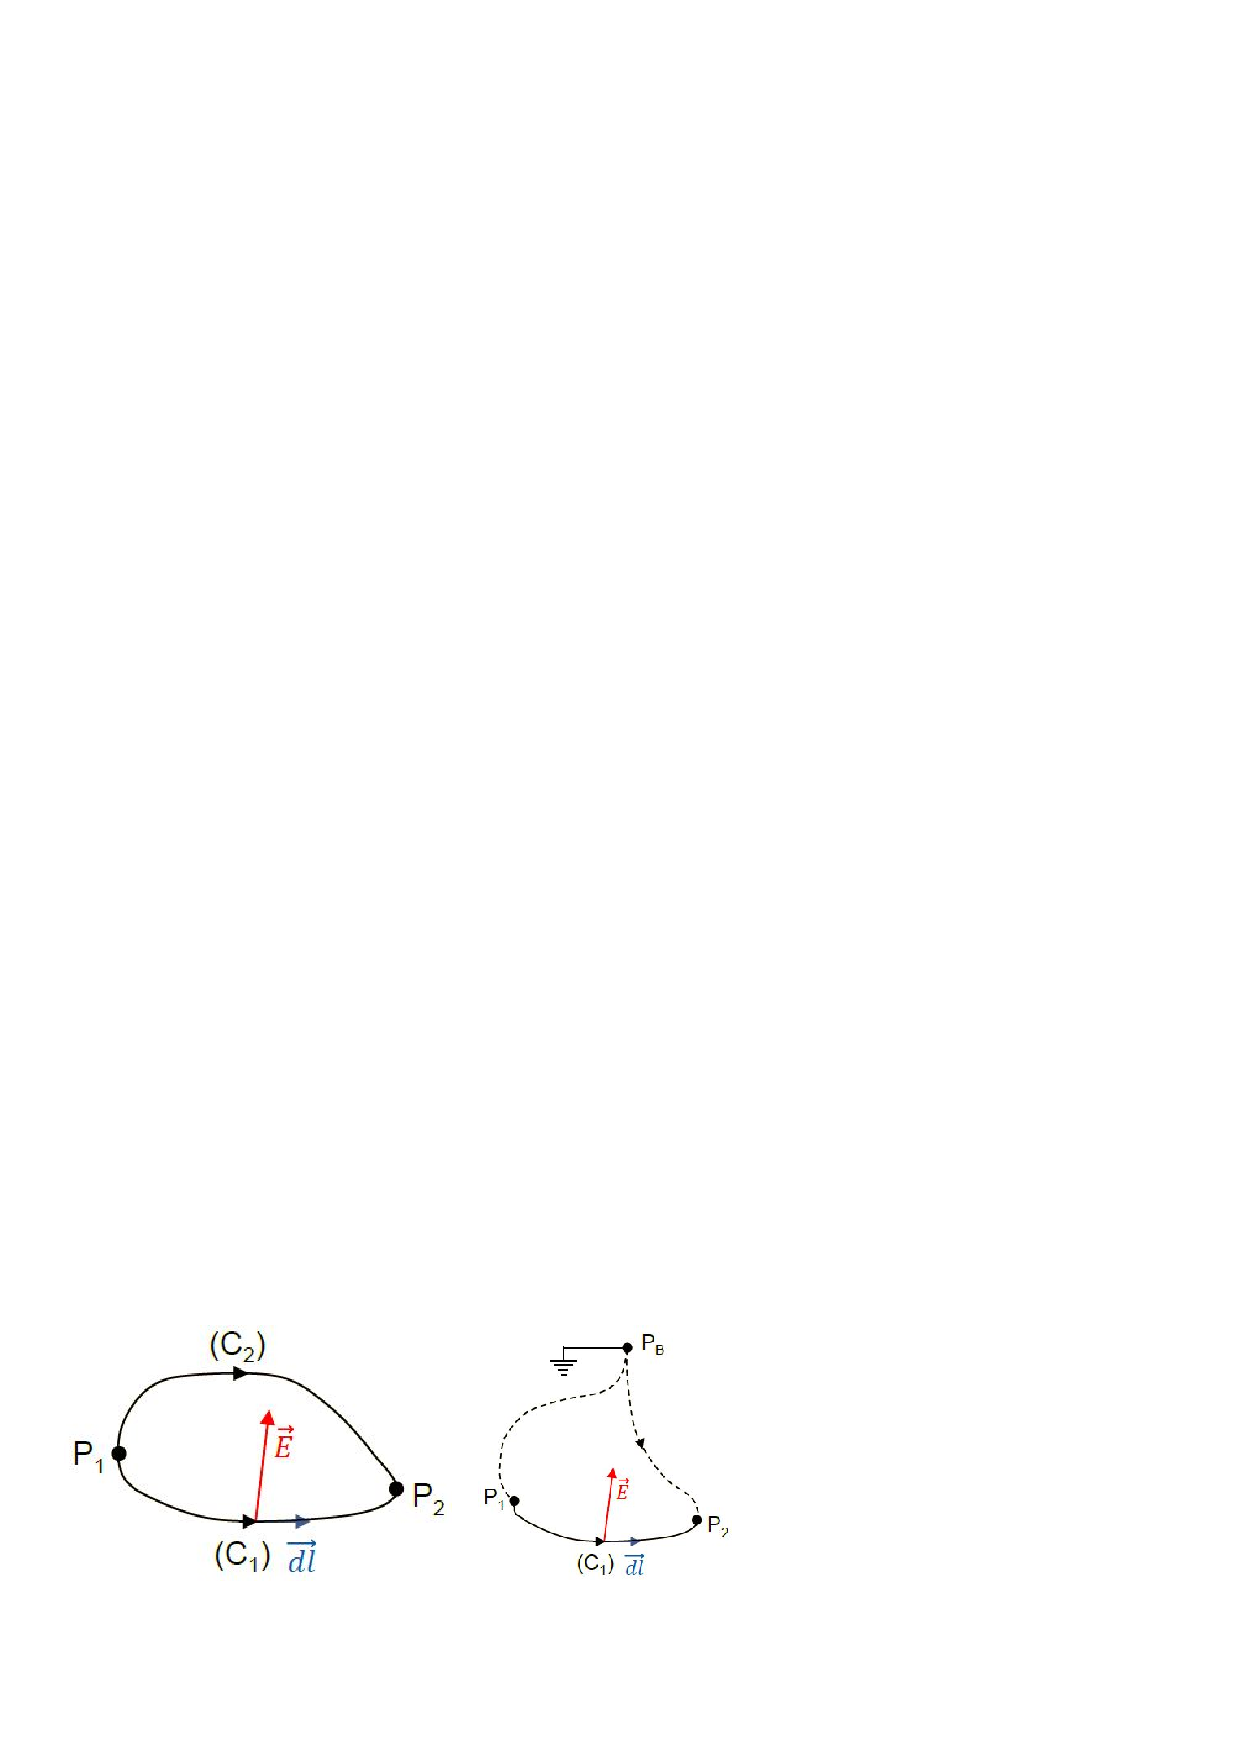
\includegraphics[width=.9\textwidth]{./images/WirbelfreiE2.pdf}
\end{minipage}
\begin{minipage}[rt]{10cm}
	\begin{equation*}
		\oint \limits_{\left(C\right)} \vec{E}\cdot \vec{dl} = 0
	\end{equation*}
	\begin{equation*}
		\int\limits_{\left(C\right)} \vec{E} \cdot \vec{dl} = \underbrace{\int_{P_1}^{P_2} \vec{E} \cdot \vec{dl}}_{C_1} - \underbrace{\int_{P_1}^{P_2} \vec{E} \cdot \vec{dl}}_{C_2} = 0
	\end{equation*}
	\begin{equation*}
		V_{P_1P_2} = \varphi_{P_1} - \varphi_{P_2} = \int_{P_1}^{P_B} \vec{E} \cdot \vec{dl} - \int_{P_1}^{P_B} \vec{E} \cdot \vec{dl} = \int_{P_1}^{P_2} \vec{E} \cdot \vec{dl}
	\end{equation*}
\end{minipage}
The line integral of an electrostatic field only depends on the start and end point. It is independent of the chosen path (conservative field).
	
\textbf{\\ \\Continuity Equation\\}
	The current through a closed oriented surface $(S)$ can be computed as
	\begin{equation*}
		I = \oiint\limits_{\left(S\right)} \vec{J} \cdot \vec{dS}
	\end{equation*}
	Because of conservation the outflowing current must be equal to the decreasing total charge in volume $(V)$.
	\begin{equation*}
		I = -\frac{dQ}{dt} = -\frac{d}{dt}\iiint\limits_{\left(V\right)} \rho \cdot dV = -\iiint\limits_{\left(V\right)} \frac{d \rho}{dt}dV
	\end{equation*}
	Both combined leads to the Continuity Equation
	\begin{equation*}
		\oiint\limits_{\left(S\right)} \vec{J} \cdot \vec{dS} = - \iiint\limits_{\left(V\right)} \frac{d\rho}{dt}dV \rightarrow \nabla \cdot \vec{J} = -\frac{\partial \rho}{\partial t}
	\end{equation*}

\textbf{\\ Ohmic law\\}
\begin{minipage}[lt]{11cm}
	\begin{tabular}{l}
		\(\displaystyle dI = \frac{dU}{R} = G \cdot dU = \sigma \cdot \frac{dA}{l} \cdot dU \) \\
		\(\displaystyle G = \sigma \cdot \frac{dA}{l} \hspace{2cm} R = \rho \cdot \frac{l}{s} \) \\
		\(\displaystyle J \cdot dA = \sigma \cdot \frac{dA}{l} \cdot E \cdot l \rightarrow J = \sigma \cdot E \) \\
		or as vectors: \(\displaystyle \vec{J} = \sigma \cdot \vec{E}\)
	\end{tabular}
\end{minipage}
\begin{minipage}[rt]{8cm}
	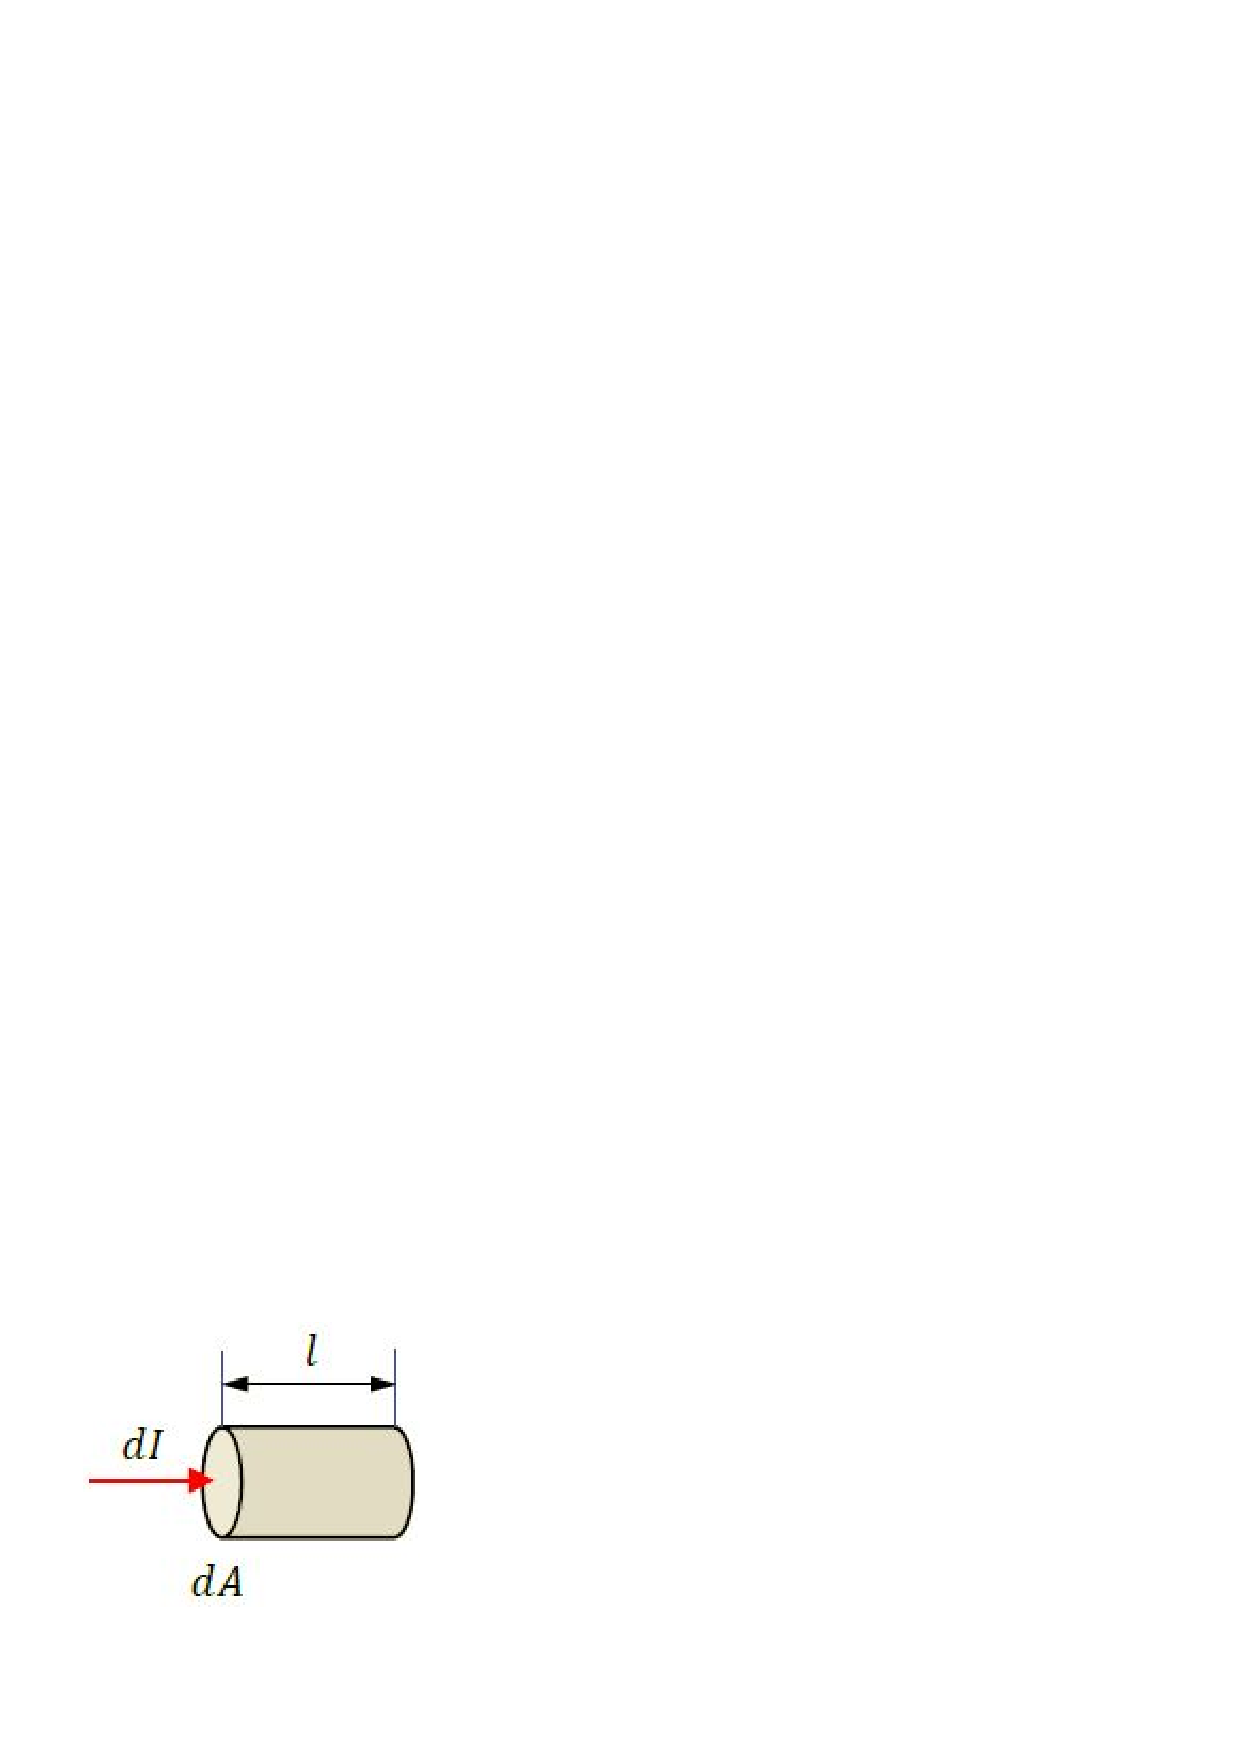
\includegraphics[width=.5\textwidth]{./images/ohmic.pdf}
\end{minipage}

\textbf{\\ \\ Skin effect\\}
\begin{tabular}{ll}
	Skin depth (where it is $e$-times lower) $[m]$: & \(\displaystyle \delta = \sqrt{\frac{2}{\omega \mu_0\sigma}} \) \\
	Skin depth for cupper at $50~Hz$: & \(\displaystyle \delta_{Cu} \approx 9mm \)
\end{tabular}


\newpage
\section{Maxwell Equations}

\subsection{Integral form}
\begin{multicols}{2}
	\textbf{Gauss's law, 1835\newline}
	\noindent The electric flux density $\vec{D} = \varepsilon \vec{E}$ through a closed oriented area $(A)$ is equal to the total electric charge $Q$ which is surrounded by this area.
	\begin{equation}
		\oiint\limits_{\left(\partial\Omega\right)} \vec{D}\left(\vec{r}\right)\cdot d\vec{S}\left(\vec{r}\right) = Q = \iiint\limits_{\left(\Omega\right)}\rho\left(\vec{r}\right)\cdot dV\left(\vec{r}\right)
		\label{eq:MaxwellInt1}
	\end{equation}
	
	\textbf{Coulomb's law, 1785\newline}
	\noindent The magnetic flux trough a closed oriented area is alway zero! This means there are no magnetic monopols.
	\begin{equation}
		\oiint\limits_{\left(\partial\Omega\right)} \vec{B}\left(\vec{r}\right)\cdot d\vec{S}\left(\vec{r}\right) = 0
		\label{eq:MaxwellInt2}
	\end{equation}
	
	\textbf{Ampère's law, 1826\newline}
	The sum of all currents through a closed oriented area can be computed as
	\begin{equation}
		\oint\limits_{\left(\partial S\right)} \vec{H}\left(\vec{r}\right)\cdot d\vec{l}\left(\vec{r}\right) = \sum_{k=1}^{N} I_k = \Theta =  \iint\limits_{\left(S\right)}\vec{J}\left(\vec{r}\right)\cdot d\vec{S}\left(\vec{r}\right)
		\label{eq:MaxwellInt3}
	\end{equation}
	
	\textbf{Faraday's law, 1831\newline}
	A time-dependent magnetic flux induces an electrical voltage.
	\begin{equation}
		u_i = \oint\limits_{\left(\partial S\right)} \vec{E}\left(\vec{r}\right)\cdot d\vec{l}\left(\vec{r}\right) = -\frac{\partial \Phi}{\partial t} = -\frac{\partial}{\partial t} \iint\limits_{\left(S\right)} \vec{B}\left(\vec{r}\right)\cdot d\vec{S}\left(\vec{r}\right)
		\label{eq:MaxwellInt4} 
	\end{equation}
\end{multicols}

\begin{figure}[h!]
	\centering
	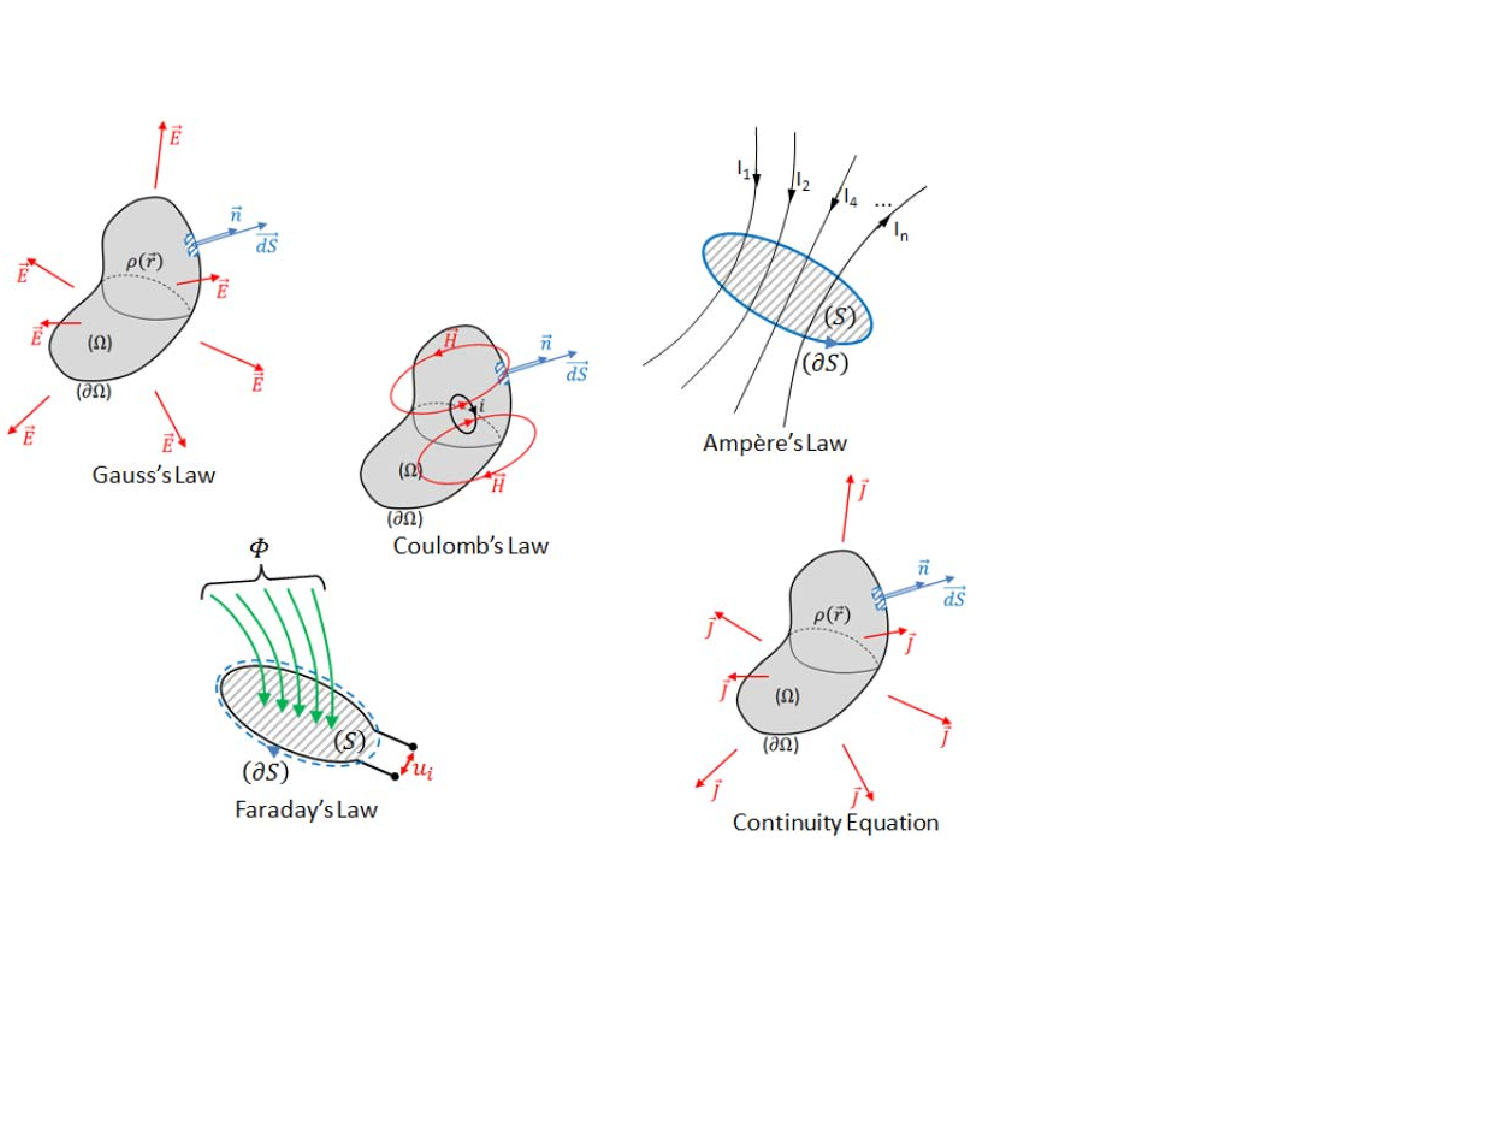
\includegraphics[width=.55\textwidth]{./images/MaxwellEqImages.pdf}
\end{figure}

\subsection{Maxwell Equations in time domain}
Using Gauss Theorem on Equation (\ref{eq:MaxwellInt1}) and (\ref{eq:MaxwellInt2}) and Stokes Theorem on (\ref{eq:MaxwellInt3}) and (\ref{eq:MaxwellInt4}) the following Maxwell Equations in time domain can be obtained as 
\begin{multicols}{2}
	\begin{equation}
		\nabla \cdot \vec{D} = \rho
		\label{eq:MaxwellDiff1_1}
	\end{equation}
	\begin{equation}
		\nabla \cdot \vec{B} = 0
		\label{eq:MaxwellDiff1_2}
	\end{equation}
	\begin{equation}
		\nabla \times \vec{H} = \vec{J} + \frac{\partial \vec{D}}{\partial t} = \sigma \vec{E} + \varepsilon \frac{\partial \vec{E}}{\partial t}
		\label{eq:MaxwellDiff1_3}
	\end{equation}
	\begin{equation}
		\nabla \times \vec{E} = - \frac{\partial \vec{B}}{\partial t}
		\label{eq:MaxwellDiff1_4}
	\end{equation}
	
	\begin{equation}
		\nabla \cdot \vec{E} = \frac{\rho}{\varepsilon}
		\label{eq:MaxwellDiff2_1}
	\end{equation}
	\begin{equation}
		\nabla \cdot \vec{H} = 0
		\label{eq:MaxwellDiff2_2}
	\end{equation}
	\begin{equation}
		\nabla \times \vec{B} = \mu\left(\vec{J} + \frac{\partial \vec{D}}{\partial t}\right)
		\label{eq:MaxwellDiff2_3}
	\end{equation}
	\begin{equation}
		\nabla \times \vec{E} = -\mu \frac{\partial \vec{H}}{\partial t}
		\label{eq:MaxwellDiff2_4}
	\end{equation}
\end{multicols}
where Equation (\ref{eq:MaxwellDiff1_3}) and (\ref{eq:MaxwellDiff2_3}) show $\vec{H} \rightarrow \vec{E}$ coupling and Equation (\ref{eq:MaxwellDiff1_4}) and (\ref{eq:MaxwellDiff2_4}) show $\vec{E} \rightarrow \vec{H}$ coupling.

\subsection{Maxwell Equations in frequency domain}
If the field sources are harmonic sinusoidal time functions, the fields must have also this time dependence if the involved materials are linear. The fields can be represented as the following complex vectors
\begin{equation*}
	\vec{F}\left(\vec{r},t\right) = \Re\{\underline{\vec{F}}\left(\vec{r}\right) \cdot e^{j\omega t}\}.
\end{equation*}
The main advantage of this approach is the following elimination of the time derivatives
\begin{equation*}
	\frac{\partial}{\partial t}\left(e{j \omega t}\right) = j \omega^\cdot e^{j \omega t}
\end{equation*}
applied to the Maxwell Equations in time domain the following is obtained
\begin{equation*}
	\nabla \cdot \underline{\vec{D}}\left(\vec{r}\right) = \underline{\rho}\left(\vec{r}\right)
\end{equation*}
\begin{equation*}
	\nabla \cdot \underline{\vec{B}}\left(\vec{r}\right) = 0
\end{equation*}
\begin{equation*}
	\nabla \times \underline{\vec{H}}\left(\vec{r}\right) = \underline{\vec{J}}\left(\vec{r}\right) + j \omega \cdot \underline{\vec{D}}\left(\vec{r}\right)
\end{equation*}
\begin{equation*}
	\nabla \times \underline{\vec{E}}\left(\vec{r}\right) = - j\omega \underline{\vec{B}}\left(\vec{r}\right)
\end{equation*}
\section{Electrostatic Analysis}

The electric and magnetic fields are completely decoupled (the field induction cease to exist). E-field and H-field exist independent from each other. \\

Since $\frac{\partial}{\partial t} = 0$, Maxwell Equations (\ref{eq:MaxwellDiff1_1}), (\ref{eq:MaxwellDiff1_4}), (\ref{eq:MaxwellDiff2_1}) and (\ref{eq:MaxwellDiff2_4}) can be written as

\begin{tabular}{ll}
	\(\displaystyle \nabla \cdot \vec{D} = \rho \) & \(\displaystyle \nabla \cdot \vec{E} = \frac{\rho}{\varepsilon} \) \\
	\(\displaystyle \nabla \times \vec{E} = 0 \) \hspace{2cm} & \(\displaystyle \nabla \times \vec{E} = 0 \) .
\end{tabular}

Since the curl of the electric field is always equal to zero, the electric field can be described as agradient of the electric scalar potential
\begin{equation*}
	\vec{E} = -\nabla \varphi \rightarrow \underbrace{\nabla \cdot \left(\varepsilon \nabla \varphi\right) = -\rho}_{\text{quasi-Poisson equation}} \rightarrow \nabla \cdot \nabla \varphi = -\frac{\rho}{\varepsilon} \rightarrow \underbrace{\Delta \varphi = -\frac{\rho}{\varepsilon}}_{\text{Poisson equation if $\varepsilon$ is everywhere equal}}
\end{equation*}
Thus, in a homogeous material the electric field is a solution of the following Poisson
\begin{equation*}
	\frac{\partial^2 \varphi}{\partial x^2} + \frac{\partial^2 \varphi}{\partial y^2} +\frac{\partial^2 \varphi}{\partial z^2} = \Delta \varphi = - \frac{\rho}{\varepsilon}
\end{equation*}
or the following Laplace equation
\begin{equation*}
	\frac{\partial^2 \varphi}{\partial x^2} + \frac{\partial^2 \varphi}{\partial y^2} +\frac{\partial^2 \varphi}{\partial z^2} = \Delta \varphi = 0
\end{equation*}
written in Cartesian coordinate. {\tiny \texttt{other coordinates in Bronstein: P.723}}

\textbf{\\ Boundary Value Problem (BVP)\\}
\begin{minipage}[lt]{11cm}
	\begin{tabular}{l}
		\(\displaystyle \frac{\partial^2 \varphi}{\partial x^2} + \frac{\partial^2 \varphi}{\partial y^2} +\frac{\partial^2 \varphi}{\partial z^2} = \Delta \varphi = - \frac{\rho}{\varepsilon}, \textrm{ in } \Omega\) \\
		\(\displaystyle \varphi = 0, \textrm{ over } \partial_{D2} \Omega \) \\
		\(\displaystyle \varphi = U, \textrm{ over } \partial_{D1} \Omega \rightarrow \) Dirichlet Boundary \\
		\(\displaystyle \frac{\partial \varphi}{\partial n} = 0, \textrm{ over } \partial_{N} \Omega \rightarrow \) Neumann Boundary \\	
		Definition Normalenableitung: \(\displaystyle \vec{n} \cdot \left(\nabla \varphi\right) = \frac{\partial \varphi}{\partial n}\)	
	\end{tabular}
\end{minipage}
\begin{minipage}[rt]{8cm}
	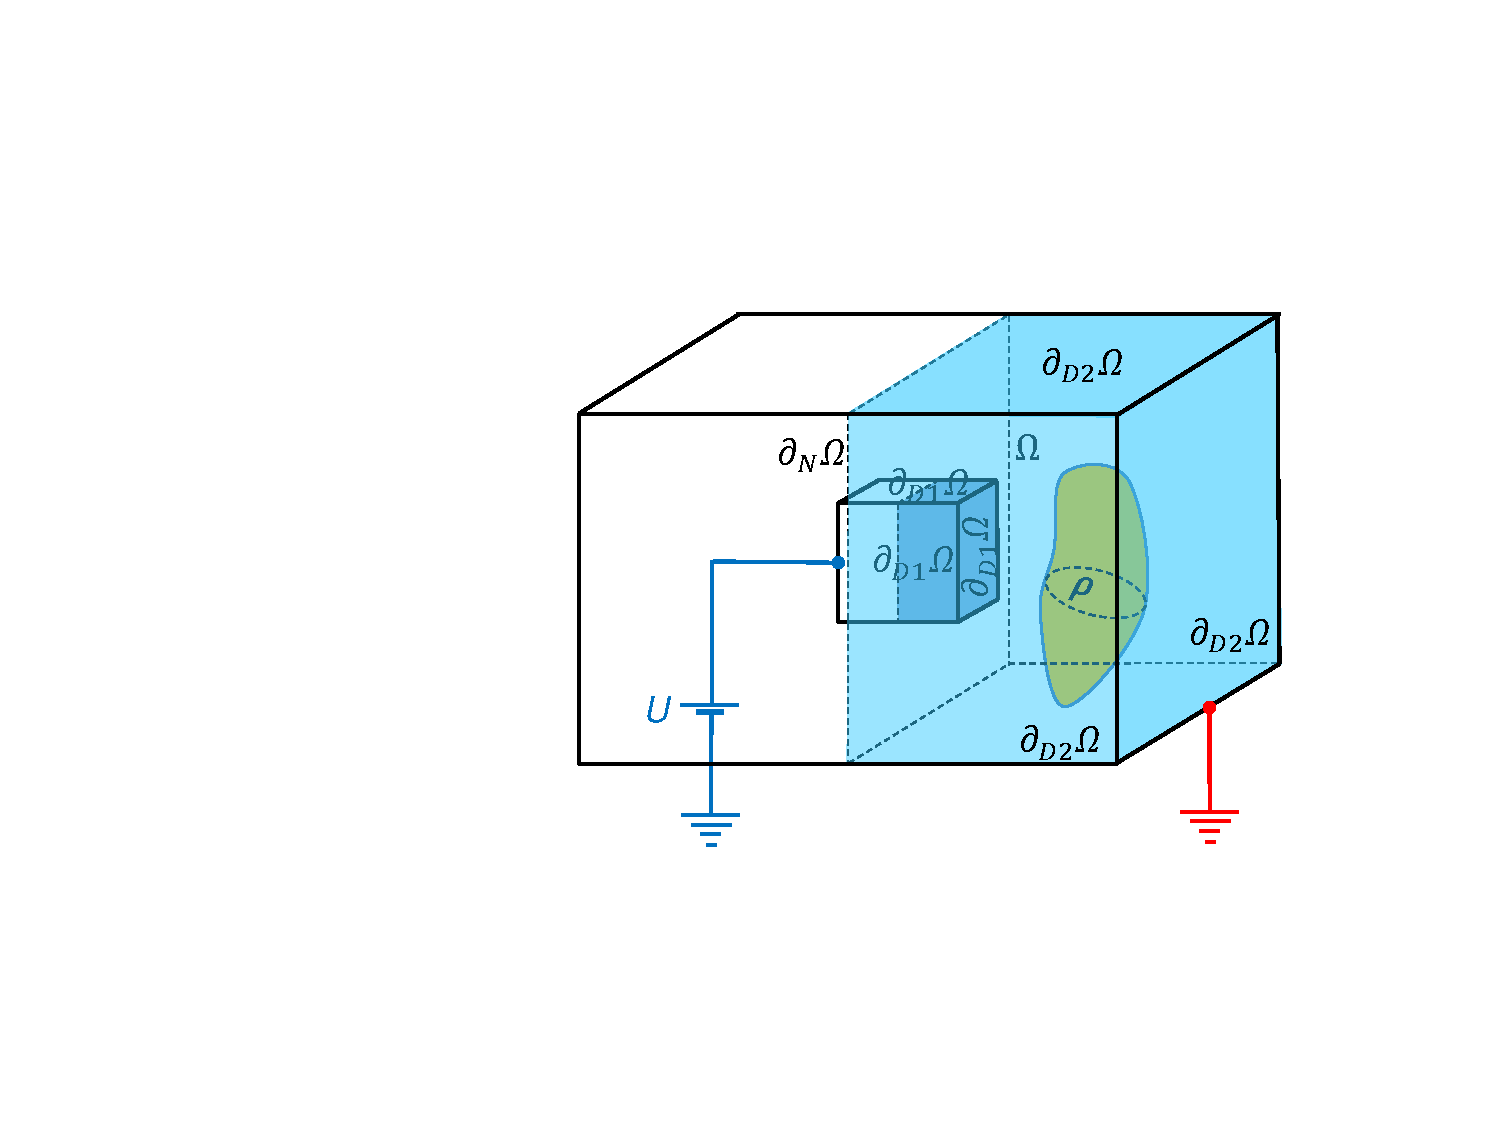
\includegraphics[width=.8\textwidth]{./images/BVP_electrostatic.pdf}
\end{minipage}
\section{Stationary Current Distribution}

Since $\frac{\partial}{\partial t} = 0$, the Continuity Equation can be written as

\begin{tabular}{ll}
	\(\displaystyle \nabla \cdot \vec{J} = -\frac{\partial \rho}{\partial t} =  0\) \\
	\(\displaystyle \nabla \cdot \vec{J} = 0 \rightarrow \nabla \cdot \left(\sigma \vec{E}\right) \rightarrow \nabla \cdot \left(\sigma V \varphi\right) = 0\) \\
\end{tabular}

Thus, the PDE is
\begin{equation*}
	\frac{\partial}{\partial x}\left(\sigma \frac{\partial \varphi}{\partial x}\right) +\frac{\partial}{\partial y}\left(\sigma \frac{\partial \varphi}{\partial y}\right)
	+\frac{\partial}{\partial z}\left(\sigma \frac{\partial \varphi}{\partial z}\right) = 0, \left(x,y,z\right) \in \Omega \subseteq R^2
\end{equation*}

\textbf{\\ Boundary Value Problem (BVP)\\}
\begin{minipage}[lt]{11cm}
	\begin{tabular}{l}
		\(\displaystyle \frac{\partial}{\partial x}\left(\sigma \frac{\partial V}{\partial x}\right) +\frac{\partial}{\partial y}\left(\sigma \frac{\partial V}{\partial y}\right)
		= 0, \left(x,y\right) \in \Omega \subseteq R^2 \) \\ \\
		\(\displaystyle \frac{\partial V}{\partial n} = 0, \left(x,y\right) \in \partial_{N1} \Omega\) \\
		\(\displaystyle \frac{\partial V}{\partial n} = \frac{I}{\sigma \cdot S_{N2}}, \left(x,y\right) \in \partial_{N2} \Omega\) \\
		\(\displaystyle V\left(x,y\right) = 0, \left(x,y\right) \in \partial_D \Omega\)\\ \\
		
		\(\displaystyle \partial_D\Omega\cup\partial_{N1}\Omega\cup\partial_{N2}\Omega = \partial\Omega = \textrm{boundary}(\Omega) \)\\
		\textbf{One BC must be a Dirichlet-BC!}
	\end{tabular}
\end{minipage}
\begin{minipage}[rt]{8cm}
	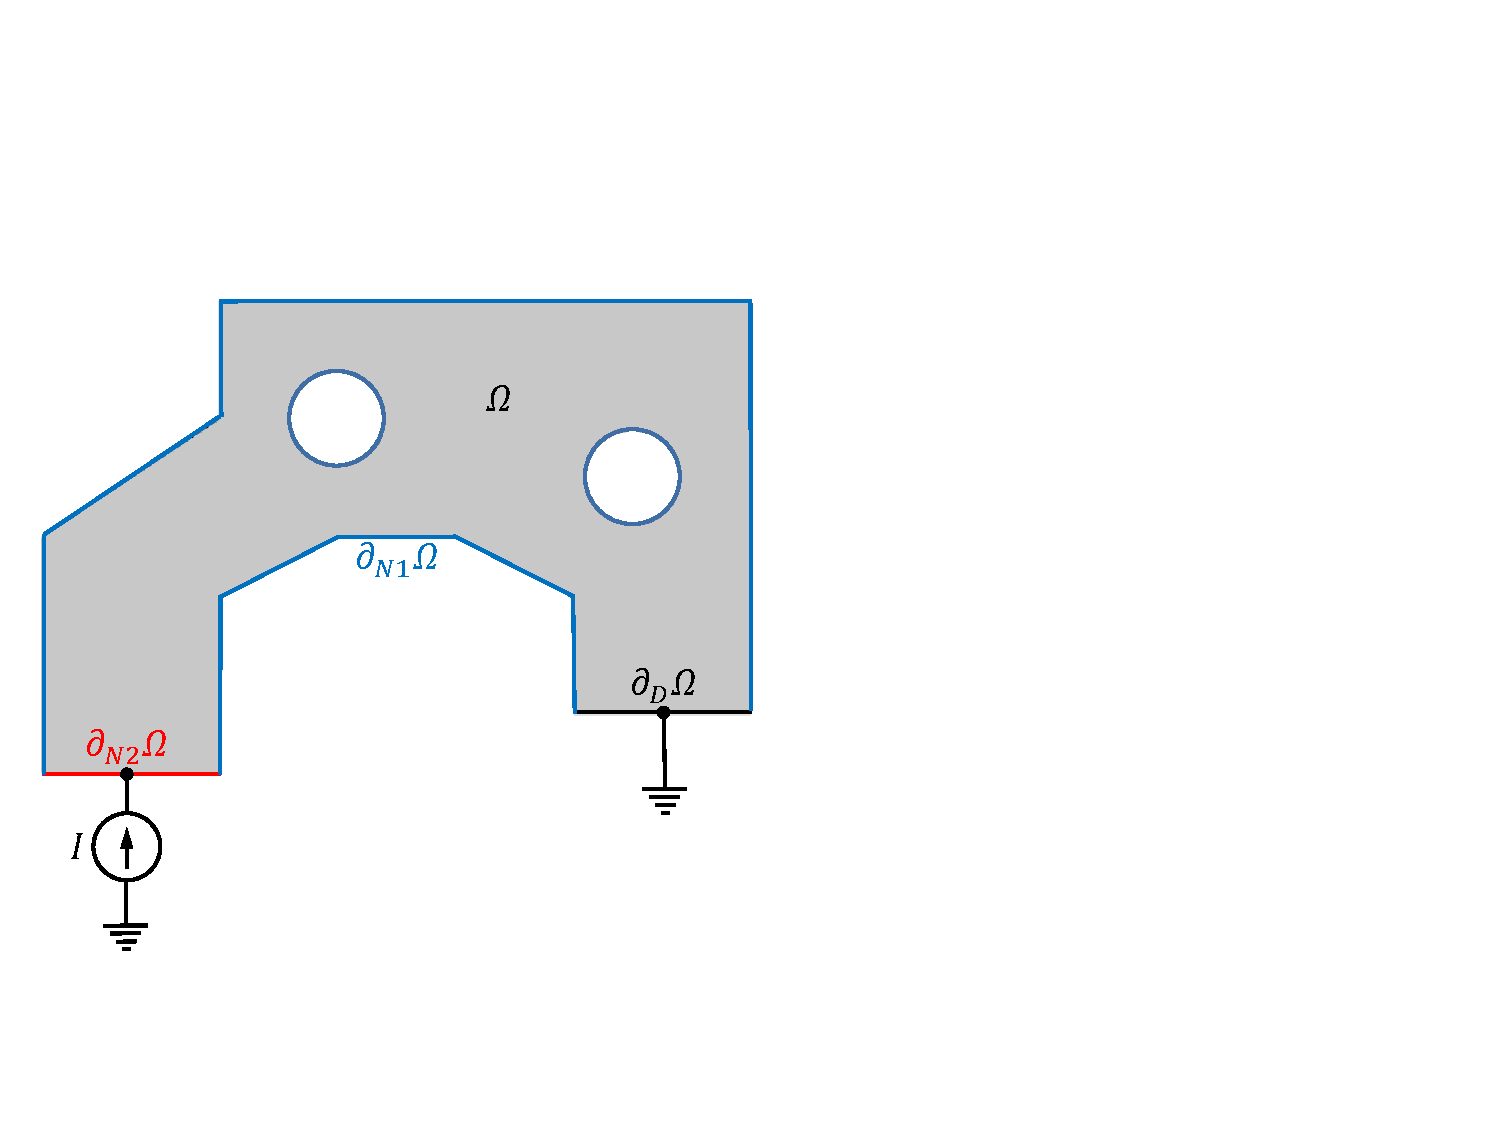
\includegraphics[width=.8\textwidth]{./images/CurrentDistribution.pdf}
\end{minipage}

\textbf{\\ \\ Post processing \\ }
\begin{tabular}{ll}
	Loss density $\left[\frac{W}{m^3}\right]$: & \(\displaystyle p_L = \vec{J} \cdot \vec{E} = \sigma \cdot \vec{E}^2 = \frac{\vec{J}^2}{\sigma} \)\\
	Total losses $[W]$: & \(\displaystyle P_L = \iiint\limits_{\left(V\right)} p_L \cdot dV = \iiint\limits_{\left(V\right)} \sigma \cdot \vec{E}^2 \cdot dV \) \\
	Resistance $[\Omega]$: & \(\displaystyle R = \frac{P_L}{I^2}\) \\
\end{tabular}
\section{Magnetostatic Analysis}

\textbf{Magnetic vector potential \\ \\}
In case when the electric field does not depend on time the following can be written
\begin{equation*}
	\nabla \cdot \vec{B} = 0
\end{equation*}
\begin{equation*}
	\nabla \times \vec{H} = \vec{J}
\end{equation*}
Due to the fact that a divergence of a curl is always equal to zero, it is possible in this case to represent the magnetic flux density as a curl of a vector function 
\begin{equation*}
	\vec{B} = \nabla \times \vec{A}
\end{equation*}
which is called the magnetic vector potential. It must fulfil the following partial differential equation
\begin{equation*}
	\underbrace{\underbrace{\nabla \times \left(\frac{1}{\mu}\underbrace{\nabla \times \vec{A}}_{\bot}\right)}_{\bot} = \vec{J}}_{||}
\end{equation*}
If the material is homogeneous, the last equation could be further simplified as 
\begin{equation*}
	\Delta\vec{A} = -\mu \vec{J}
\end{equation*}

\textbf{\\ Boundary Value Problem (BVP)\\}
\begin{minipage}[lt]{11cm}
	\begin{tabular}{l}
		\textbf{3D:} \\
		\(\displaystyle \nabla \times \left(\frac{1}{\mu}\nabla \times \vec{A}\right) = \vec{J} \) \\
		\(\displaystyle \vec{n} \times \vec{A} = 0, \textrm{ over } \partial_D\Omega \) \\
		\(\displaystyle \vec{n} \times \nabla \times \vec{A} = 0,\textrm{ over } \partial_N\Omega \) \\
		\textbf{2D planar (from book):} \\
		\(\displaystyle -\frac{\partial }{\partial x} \left(\frac{1}{\mu} \frac{\partial A_z}{\partial x}\right) - \frac{\partial }{\partial y} \left(\frac{1}{\mu} \frac{\partial A_z}{\partial y}\right) = J_z \) \\
		\(\displaystyle A_z = 0, \textrm{ over } \partial_D\Omega \) \\
		\(\displaystyle \frac{\partial A_z}{\partial n} = 0, \textrm{ over } \partial_N\Omega\) \\
		\textbf{First, the current density $\vec{J}$ must be computed to obtain a magnetostatic solution.}
	\end{tabular}
\end{minipage}
\begin{minipage}[rt]{8cm}
	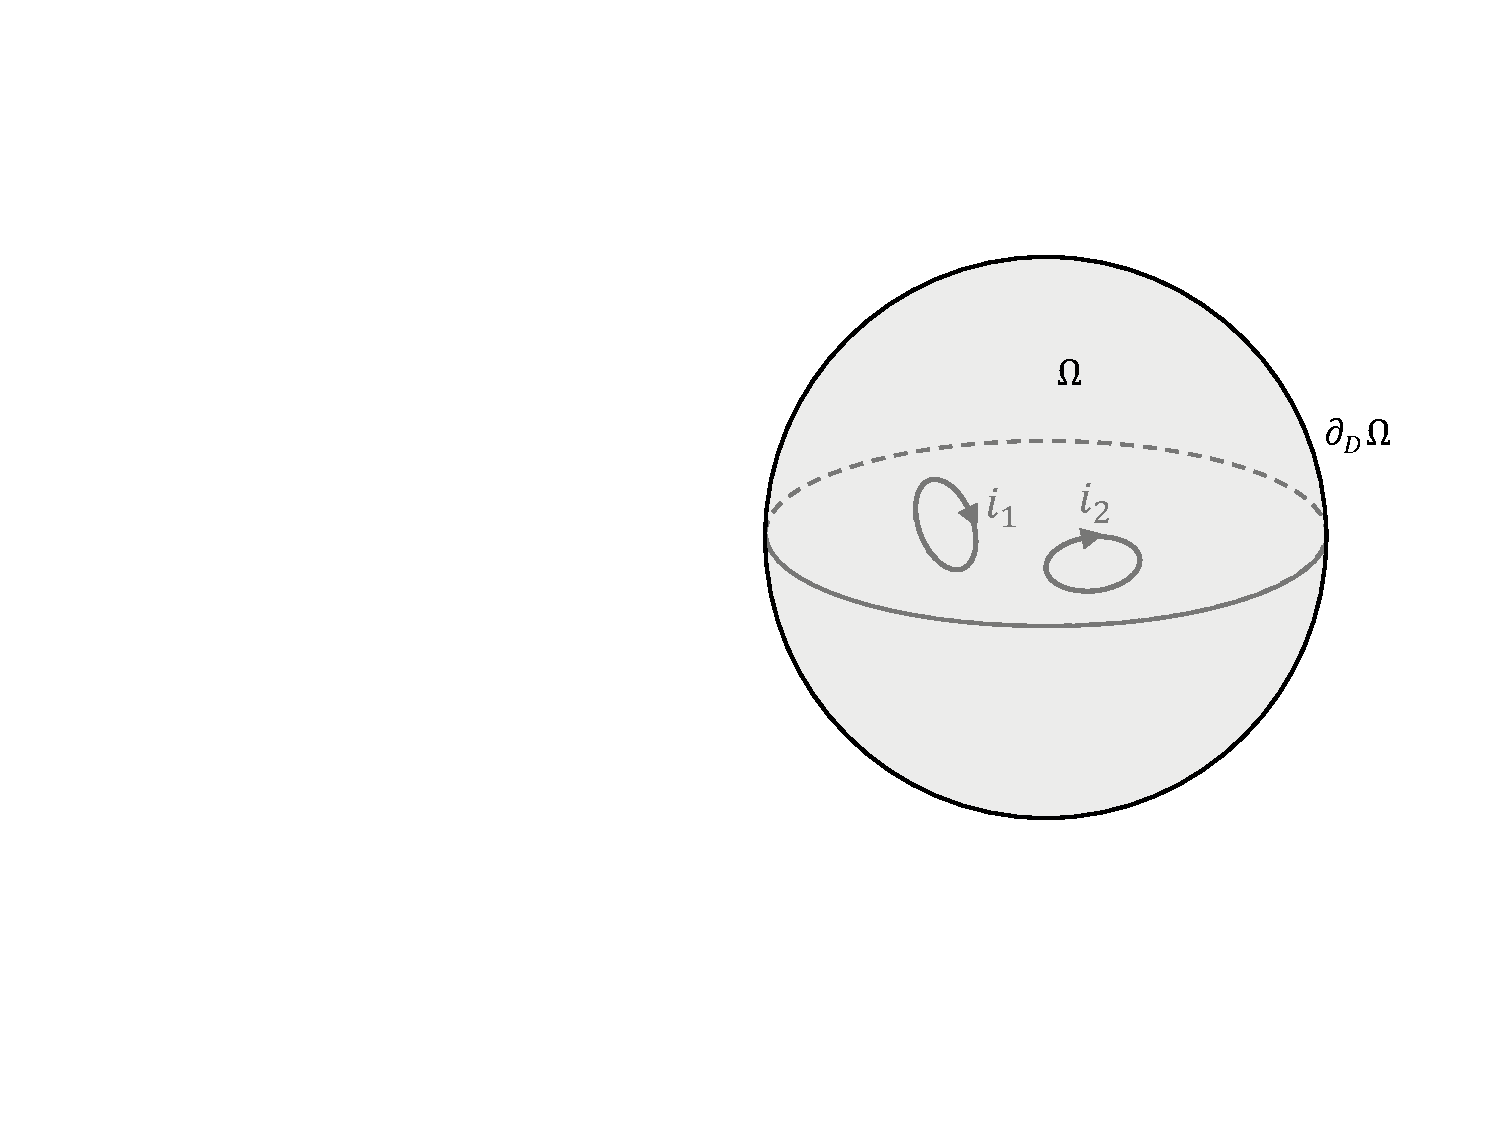
\includegraphics[width=.8\textwidth]{./images/BVP_magnetostatic.pdf}
\end{minipage}

\textbf{\\ \\ Post processing \\ }
\begin{tabular}{ll}
	Magnetic energy $\left[Ws\right]$: & \(\displaystyle W_m = \frac{1}{2} \iiint\limits_{\left(\Omega\right)} \vec{B} \cdot \vec{H} dV \) \\
	Inductivity $\left[H\right]$: & \(\displaystyle \frac{2 W_m}{I^2} \) 
\end{tabular}
\section{Electroquasistatic Analysis}
If the induced electric field can be neglected and the displacement currrent \textbf{cannot} (coupling only in one direction $\vec{E} \rightarrow \vec{H}$), the conditions for electroquasistatic analysis are established \\
\begin{equation*}
	\nabla \times \vec{E} = -\frac{\partial \vec{B}}{\partial t} \approx 0
\end{equation*}
\begin{equation*}
	\vec{J} = \underbrace{\vec{J}_s}_{\textrm{source current}} + \underbrace{\sigma \vec{E}}_{\textrm{internal current (conduction)}} + \underbrace{\varepsilon \frac{\partial \vec{E}}{\partial t}}_{\textrm{displacement current (polarization)}}
\end{equation*}
Generally speaking, the
PDE can be obtained with continuity equation $\nabla \cdot \vec{J} = 0$
\begin{equation*}
	\nabla \cdot \left(\sigma \nabla \varphi\right) + \nabla \cdot \left(\varepsilon \frac{\partial}{\partial t}\nabla \varphi\right) = \nabla \cdot \left(\vec{J}_s\right), \textrm{ in } \Omega
\end{equation*}
and PDE in frequency domain
\begin{equation*}
	\nabla \cdot \left(\sigma \nabla \underline{\varphi}\right) + \nabla \cdot \left( j \omega \varepsilon \nabla \underline{\varphi}\right) = \nabla \cdot \left(\vec{J}_s\right), \textrm{ in } \Omega.
\end{equation*}

\textbf{\\ Boundary Value Problem (BVP)\\}
\begin{minipage}[lt]{11cm}
	\begin{tabular}{l}
		\(\displaystyle \varphi = U, \textrm{ over } \partial_{D1}\Omega \) \\
		\(\displaystyle \varphi = 0, \textrm{ over } \partial_{D2}\Omega \) \\
		\(\displaystyle \frac{\partial \varphi}{\partial n} = 0, \textrm{ over } \partial_{N}\Omega \)
	\end{tabular}
\end{minipage}
\begin{minipage}[rt]{8cm}
	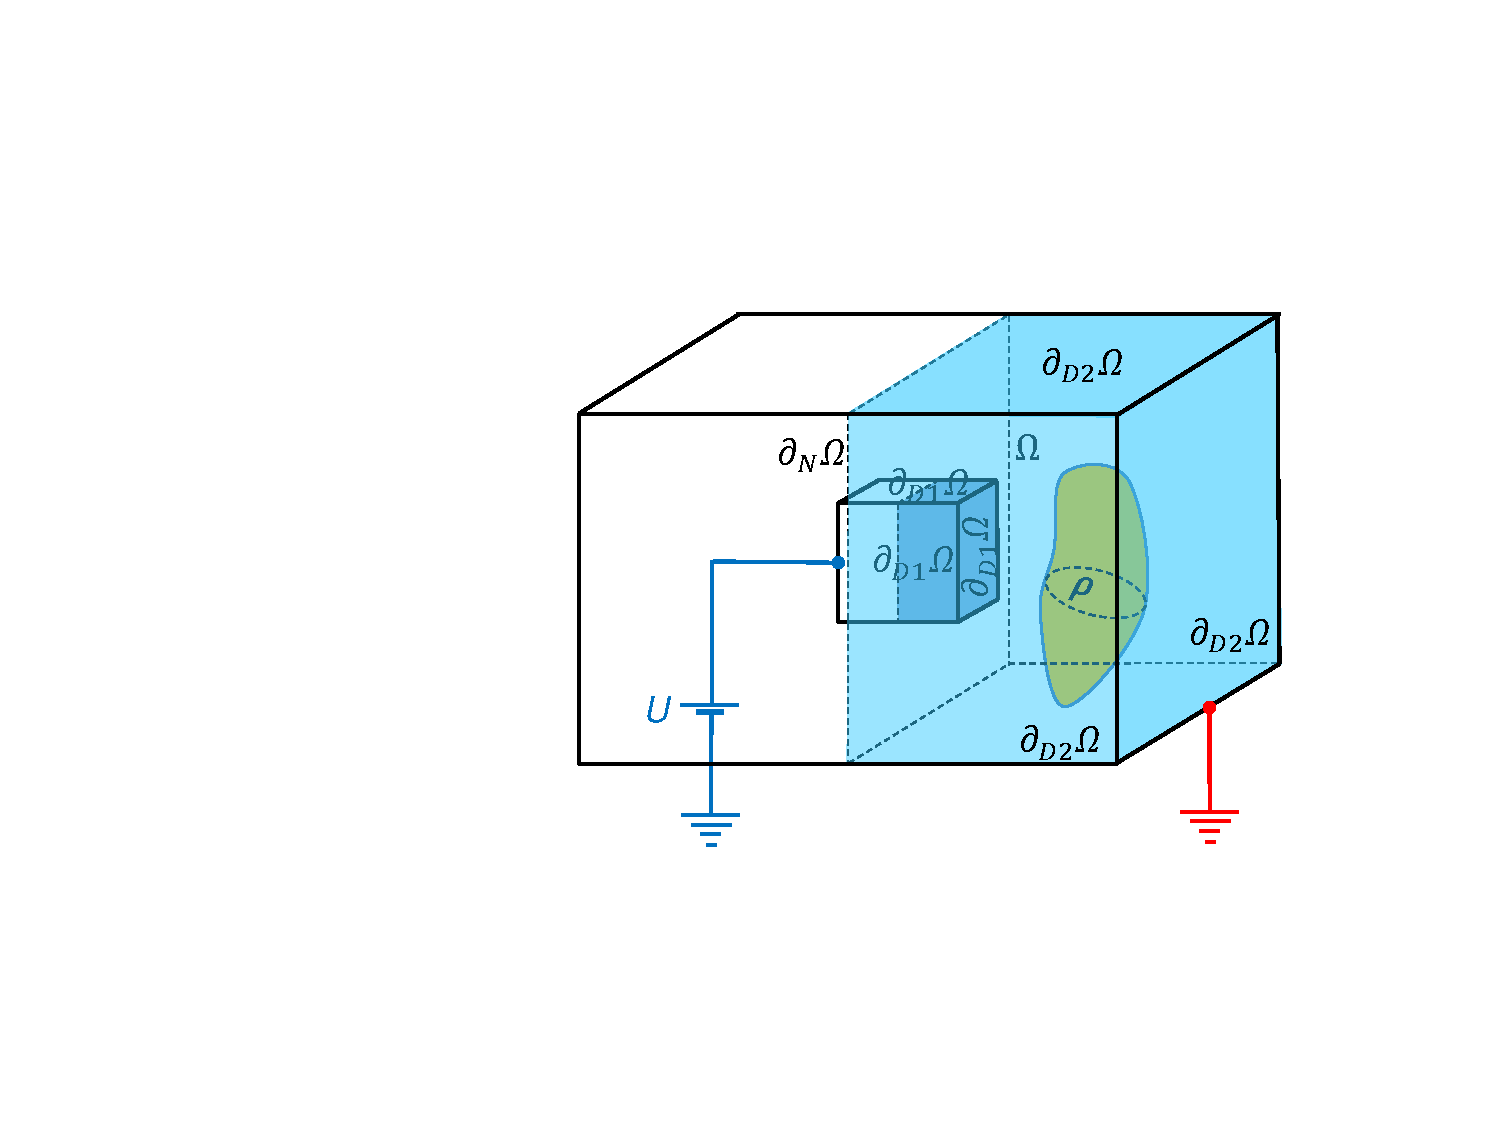
\includegraphics[width=.6\textwidth]{./images/BVP_electrostatic.pdf}
\end{minipage}
\section{Magnetoquasistatic Analysis}
In the frequency domain the used equations look like 
\begin{equation*}
	\nabla \times \vec{E} = -j\omega\mu\underline{\vec{H}}
	\hspace{1.6cm}
	\nabla \times \vec{H} = \vec{J} + j\omega \varepsilon \vec{E}
\end{equation*}
Since $\mu$ is much higher than $\varepsilon$, the term $j\omega\mu$ is dominant for smaller frequency. Therefor, $\frac{\partial \vec{D}}{\partial t} \approx 0$ which means thath the induced magnetic field due to the displacement current can be neglected (coupling only in one direction $\vec{B} \rightarrow \vec{E}$) which leads to the following equations in time domain
\begin{equation*}
	\nabla \times \vec{E} = -\frac{\partial \vec{B}}{\partial t}
	\hspace{2cm}
	\nabla \times \vec{H} = \vec{J}
	\hspace{2cm}
	\nabla \cdot \vec{B} = 0.
\end{equation*}
Since the divergence of the magnetic flux density is always equal to zero, the B-field can be described as
\begin{equation*}
	\vec{B} = \nabla \times \vec{A}
\end{equation*}
which leads to 
\begin{equation*}
	\nabla \times \left(\frac{1}{\mu} \nabla \times \vec{A}\right) = \vec{J} = \underbrace{\vec{J}_s}_{\textrm{source current density}} + \sigma \vec{E}.
\end{equation*}
With $\vec{E} = - \frac{\partial \vec{A}}{\partial t}$ this can be further simplified to
\begin{equation*}
	\nabla \times \left(\frac{1}{\mu}\nabla \times \vec{A}\right) + \underbrace{\sigma \frac{\partial \vec{A}}{\partial t}}_{\textrm{eddy currents}} = \vec{J}_s
\end{equation*}
If the material is homogeneous this equation can be written in time or frequency domain as 
\begin{equation*}
	\Delta\vec{A} -\mu\sigma\frac{\partial \vec{A}}{\partial t} = -\mu \vec{J}_s, (x,y,z)\in \Omega
	\hspace{2cm}
	\Delta\vec{A} - j\omega\mu\sigma\underline{\vec{A}} = -\mu\underline{\vec{J}_s}, (x,y,z)\in \Omega
\end{equation*}

\textbf{\\ Boundary Value Problem (BVP)\\}
\begin{minipage}[lt]{11cm}
	\begin{tabular}{l}
		Magnetic insulation: \\
		\(\displaystyle n \times \vec{A} = 0,(x,y,z)\in \partial_D\Omega\)\\
		Boundary between to materials: \\
		\(\displaystyle n \times \vec{A}_1 = n \times \vec{A}_2), (x,y,z) \in \partial_N\Omega \) \\
		BVP (right example): \\
		\(\displaystyle \underline{A}_z = 0, \mathrm{ on } \partial_D\Omega \) \\
		\(\displaystyle \frac{\partial \underline{A}_z}{\partial n} = 0, \textrm{ o n} \partial_N\Omega \)
	\end{tabular}
\end{minipage}
\begin{minipage}[rt]{8cm}
	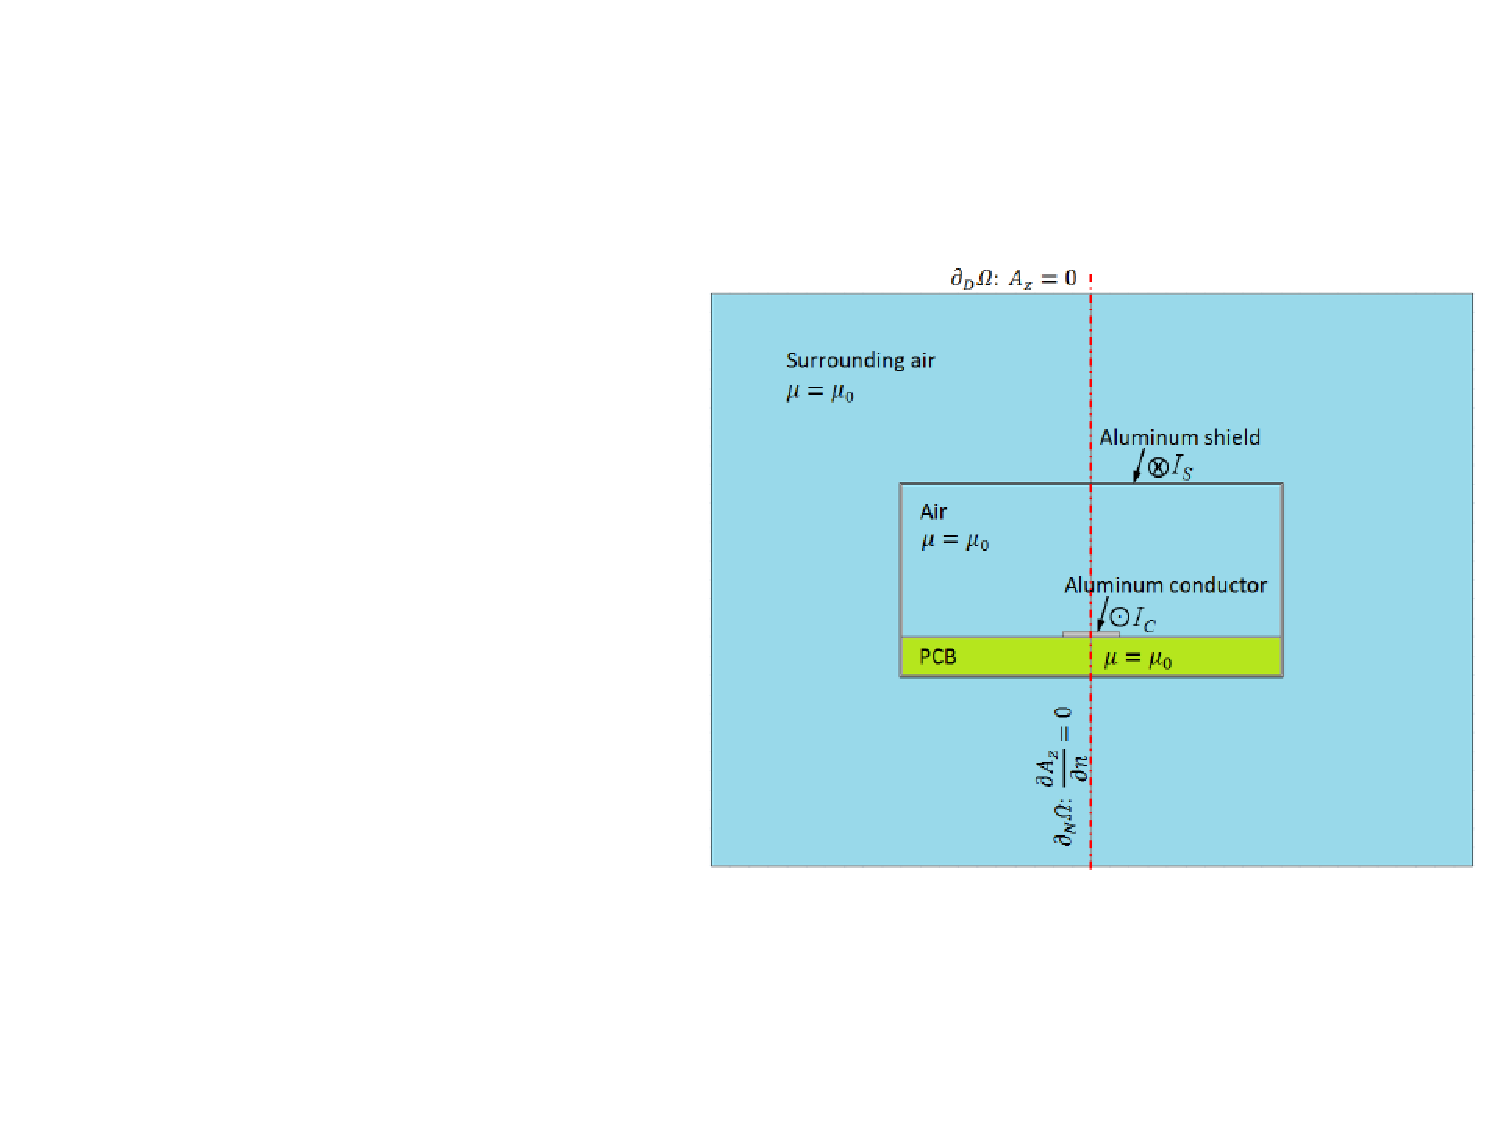
\includegraphics[width=.8\textwidth]{./images/BVP_magnetosquasistatic.pdf}
\end{minipage}
\newpage
\section{Electromagnetic Waves}
Propagation of electromagnetic waves is described by the complete set of Maxwell equations either in frequency- or time domain. However, it is a common practice to derive and solve a single electromagnetic wave equation (E-field \textbf{or} H-field).\\

E-Field wave equations in time and frequency domain:
\begin{equation*}
	\Delta \vec{E} - \underbrace{\mu\sigma\frac{\partial \vec{E}}{\partial t}}_{\textrm{losses}} - \underbrace{\mu\varepsilon\frac{\partial^2 \vec{E}}{\partial t^2}}_{\textrm{wave}} = 0
	\hspace{2cm}
	\Delta \underline{\vec{E}} - j\omega\mu\sigma\underline{\vec{E}} + \omega^2\mu\varepsilon\underline{\vec{E}} = 0
\end{equation*}
H-Field wave equations in time and frequency domain:
\begin{equation*}
	\Delta\vec{H} - \underbrace{\mu\sigma\frac{\partial \vec{H}}{\partial t}}_{\textrm{losses}} - \underbrace{\mu\varphi\frac{\partial^2 \vec{H}}{\partial t^2}}_{\textrm{wave}} = 0
	\hspace{1.8cm}
	\Delta \underline{\vec{H}} - m\omega\mu\sigma\underline{\vec{H}} + \omega^2\mu\varepsilon\underline{\vec{H}} = 0
\end{equation*}

\textbf{\\ Boundary Value Problem (BVP)\\}
\begin{minipage}[lt]{11cm}
	\begin{tabular}{l}
		\(\displaystyle \vec{n} \times \vec{E} = 0, \textrm{ over }\partial_{\mathrm{PEC}}\Omega \) \\
		\(\displaystyle \vec{n}_1 \times \left(\nabla \times \vec{E}\right) + jk_z\vec{n}_1 \times \left(\vec{n}_1 \times \vec{E}\right) = \) \\
		\(\displaystyle \hspace{2cm}2jk_z \vec{n}_1 \times \left(\vec{n}_1 \times \vec{E}_i\right), \textrm{ over } \partial_{\mathrm{PORT1}}\Omega \) \\
		\(\displaystyle \vec{n}_2 \times \left(\nabla \times \vec{E}\right) + jk_0\vec{n}_2 \times \left(\vec{n}_2 \times \vec{E}\right) = 0, \textrm{ over } \partial_{\textrm{PORT2}}\Omega \) \\
		\(\displaystyle k_z = \sqrt{\omega^2\mu\varepsilon-k_t^2} \) \\
		\(\displaystyle k^2_{tmn} = \left(\frac{m\pi}{a}\right)^2 + \left(\frac{n\pi}{b}\right) ^2\) \\
	\end{tabular}
\end{minipage}
\begin{minipage}[rt]{8cm}
	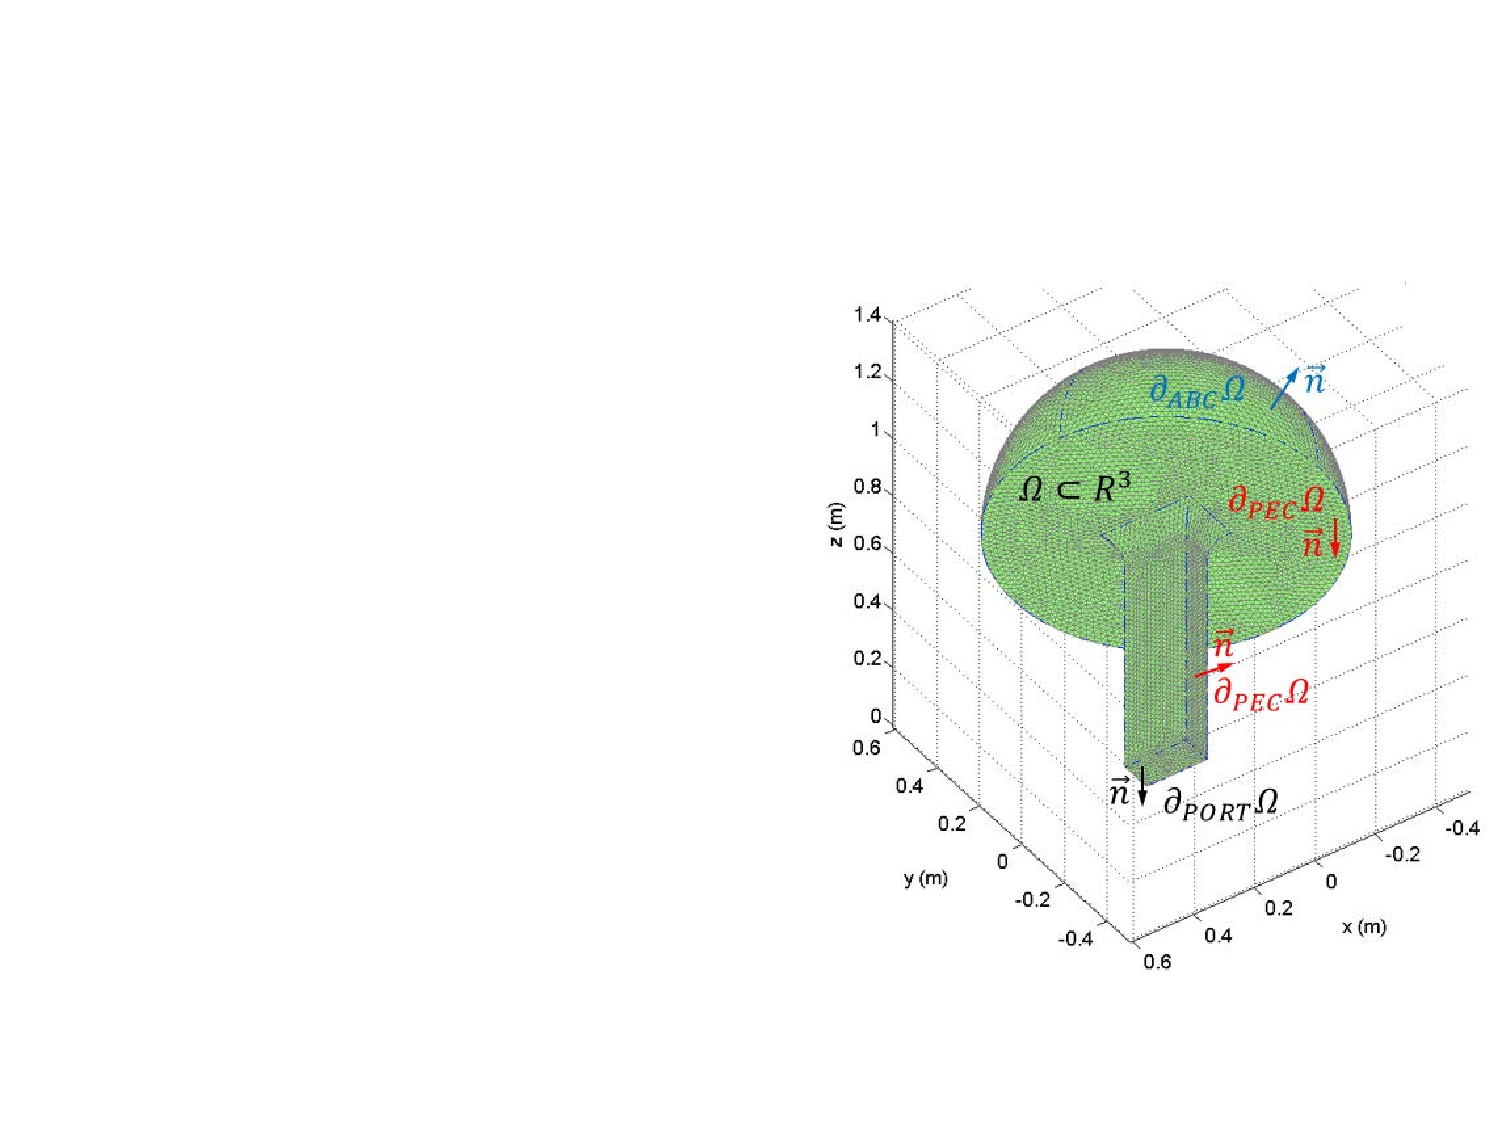
\includegraphics[width=.8\textwidth]{./images/BVP_wave.pdf}
\end{minipage}
\section{Boundary Conditions (BC)}
\subsection{Interface Conditions}
\begin{minipage}[rt]{8cm}
	\begin{tabular}{l}
		\(\displaystyle \left(\vec{D}_1 - \vec{D}_2\right) \cdot \vec{n} = \rho_S\) \\
		\(\displaystyle\left(\vec{B}_1 - \vec{B}_2\right) \cdot \vec{n} = 0\)\\
		\(\displaystyle\left(\vec{H}_2 - \vec{H}_1\right) \times \vec{n} =\vec{J}_S\) \\
		\(\displaystyle\left(\vec{E}_2 - \vec{E}_1\right) \times \vec{n} = 0\)\\
	\end{tabular}
\end{minipage}
\begin{minipage}[lt]{11cm}
	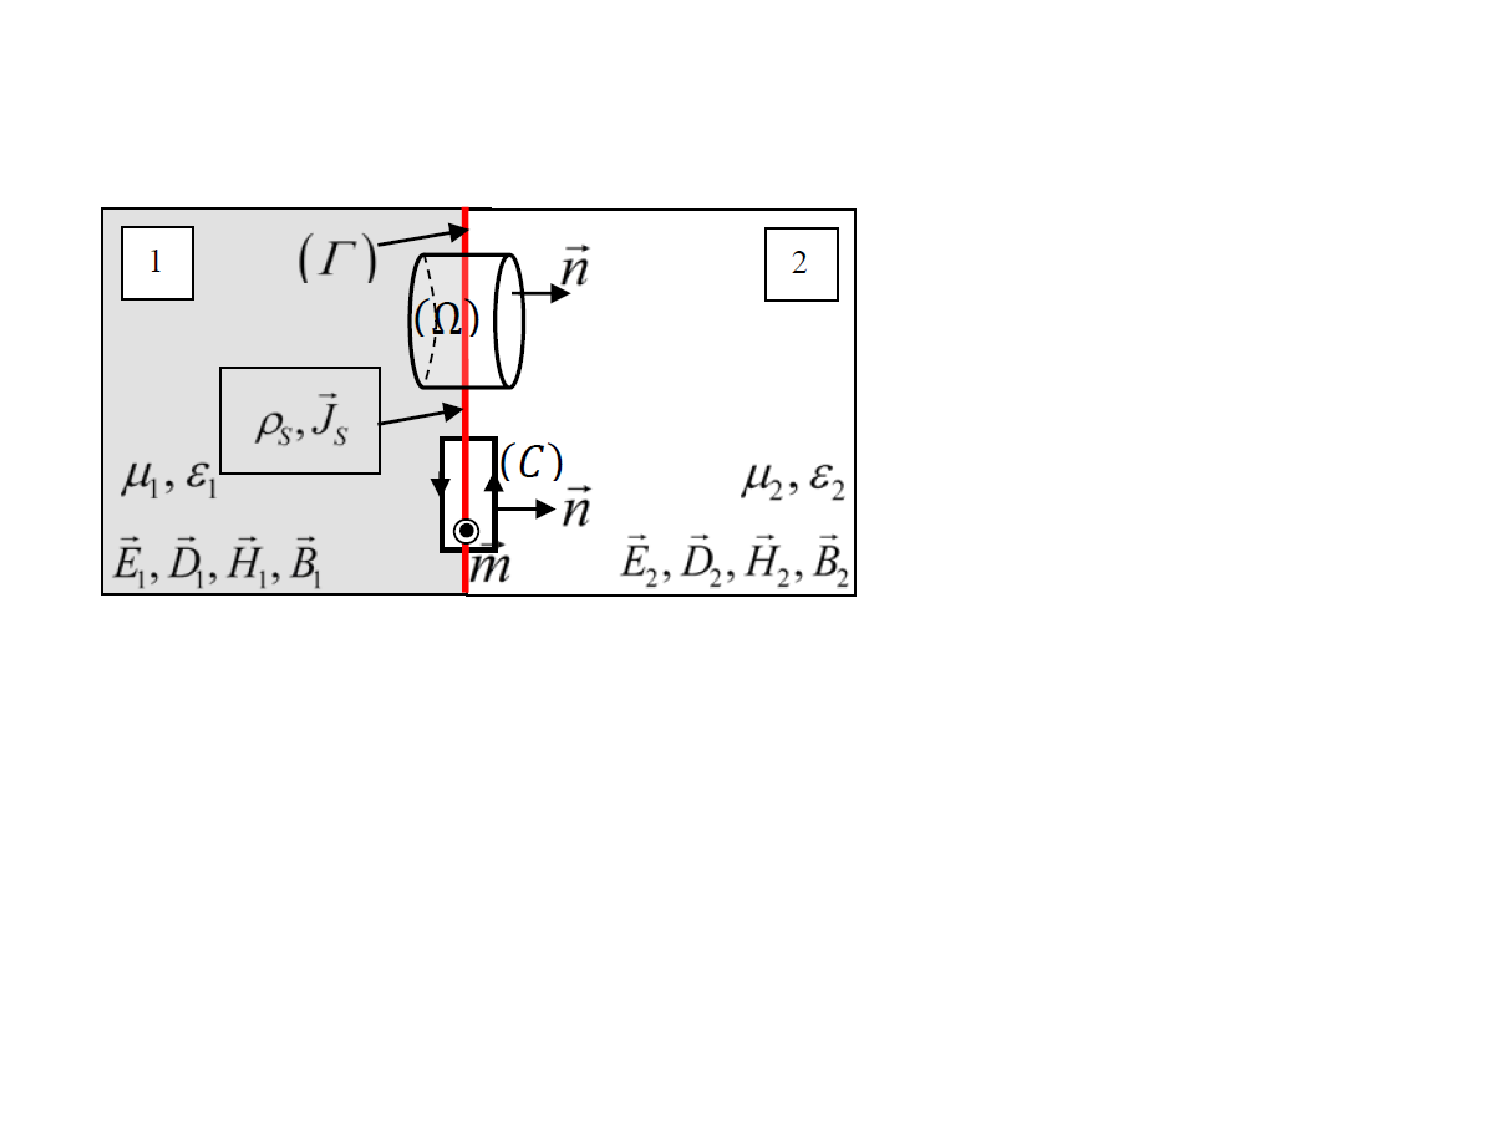
\includegraphics[width=.6\textwidth]{./images/InterfaceConditions.pdf}\\
\end{minipage}
The above interface conditions show the field behavior over the border between two different materials. \newline
The normal flux density continuity conditions can be derived by integrating Equations (\ref{eq:MaxwellInt1}) and (\ref{eq:MaxwellInt2}) over the cylinder $\Omega$ depicted above. \newline
The tangential field continuity conditions can be proven by integrating Equations (\ref{eq:MaxwellInt3}) and (\ref{eq:MaxwellInt4}) along the contour $C$ shown above.
\newpage
\section{FEM}

\subsection{General 2D Form}
The PDE of second order (strom form) along with the corresponding BCs form the BVP
\begin{equation*}
	-\frac{\partial }{\partial x}\left(a_x \frac{\partial \Phi}{\partial x}\right) - \frac{\partial }{\partial y}\left(\frac{\partial \Phi}{\partial y}\right) + \beta \Phi = f, (x,y) \in \Omega \subseteq R^2
\end{equation*}
\begin{equation*}
	\Phi(x,y) = p, (x,y) \in \partial_D\Omega
\end{equation*}
\begin{equation*}
	\left(a_x \frac{\partial \Phi}{\partial x}\cdot \vec{e_x} + a_y \frac{\partial \Phi}{\partial y} \cdot \vec{e_y}\right) \cdot \vec{n} = q, (x,y) \in \partial_N\Omega
\end{equation*}
\begin{equation*}
	\partial_D\Omega \cup \partial_N\Omega = \partial\Omega = \textrm{boundary}(\Omega)
\end{equation*}
where $\Omega$ is the computational domain, $\alpha$ and $\beta$ are constants representing the material properties, $f$ is a predefined source term, $\vec{n}$ is a normal outward unit vector at a certain point on the Neumann boundary, and $\Phi$ is an unknown function. \\

The method of weighted residuals (approximation to $0$) is used in order to abtain an equivalent integral form (weak form as it is first order) of the 2D BVP. With some (s)magic the equivalent integral form becomes:
\begin{equation*}
	\iint\limits_{\left(\Omega\right)} \nabla w_i \cdot \left(a_x \frac{\partial \Phi}{\partial x} \vec{e_x} + a_y \frac{\partial \Phi}{\partial y} \vec{e_y}\right) d\Omega + \iint\limits_{\left(\Omega\right)} w_i\beta\Phi d\Omega - \iint\limits_{\left(\Omega\right)} w_i f d\Omega  - \int\limits_{\left(\partial_N\Omega\right)} w_i \cdot q \cdot dl = 0
\end{equation*}
The name 'weak' comes from the fact that this form consists of only partial derivatives of first oder, while the partial derivatives in the BVP are of second order ('strong' form).

\subsection{Meshing}
The goal for meshing is to get from complex geometries to large numbers of elements with simple geometry (triangles, quadrilaterals).\newline

With a subdivison of
\begin{equation*}
	\Omega = \bigcup\limits_{e=1}^{N_e} \Omega^e
\end{equation*}
where the superscript $e$ refers to a local approximation within the element $e$, the original weak form becomes
\begin{equation*}
	\sum_{e=1}^{N_e} \iint\limits_{\left(\Omega^e\right)} \alpha^e \nabla {w_i}^e \cdot \nabla \Phi^e d\Omega + \sum_{e=1}^{N_e} \iint\limits_{\left(\Omega^e\right)} {w_i}^e\beta^e\Phi^e d\Omega - \sum_{e=1}^{N_e} \iint\limits_{\left(\Omega^e\right)}{w_i}^e f^e d\Omega  - \sum_{e} \int\limits_{\partial \Omega^e} {w_i}^e q^e dl = 0
\end{equation*} 

\begin{minipage}[rt]{12cm}
	\begin{tabular}{l}
		Linear approximation of the unknown function over the element: \\
		\(\displaystyle \Phi^e(x,y) = a + bx + cy \) \\
		Expressed wit respect to the nodal values: \\
		\(\displaystyle {\Phi_1}^e = a + b{x_1}^e + c{y_1}^2 \) \\
		\(\displaystyle {\Phi_2}^e = a + b{x_2}^e + c{y_2}^2 \) \\
		\(\displaystyle {\Phi_3}^e = a + b{x_3}^e + c{y_3}^2 \) \\
		\(\displaystyle \Rightarrow 
			\begin{bmatrix}
				{\Phi_1}^e \\
				{\Phi_2}^e \\
				{\Phi_3}^e
			\end{bmatrix} 
			=
			\begin{bmatrix}
				1 & {x_1}^e & {y_1}^e \\
				1 & {x_2}^e & {y_2}^e \\
				1 & {x_3}^e & {y_3}^e 
			\end{bmatrix}
			\cdot
			\begin{bmatrix}
				a \\
				b \\
				c
			\end{bmatrix}
			= 
			\begin{bmatrix}
				S^e 
			\end{bmatrix}
			\cdot 
			\begin{bmatrix}
				a \\
				b \\
				c
			\end{bmatrix} \) \\
	\end{tabular}
\end{minipage}
\begin{minipage}[lt]{8cm}
	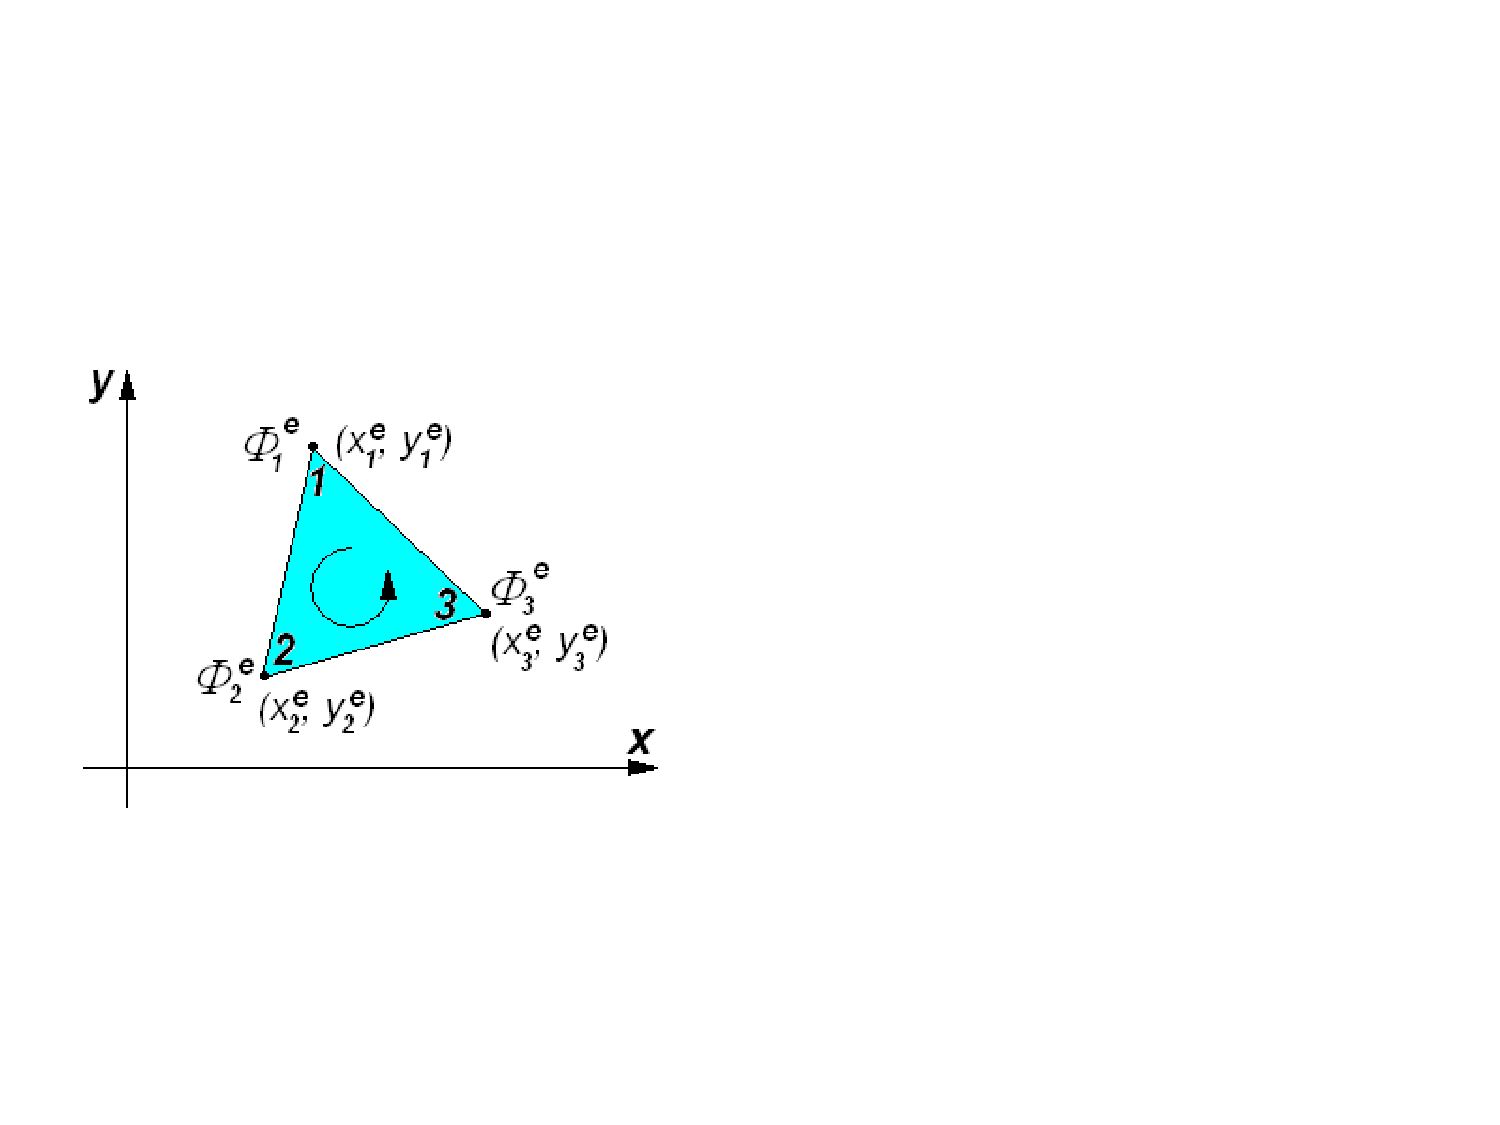
\includegraphics[width=.8\textwidth]{./images/nodes.pdf}\\
\end{minipage}
This system can be solved as
\begin{equation*}
	\begin{bmatrix}
		a \\
		b \\
		c
	\end{bmatrix}
	= 
	\begin{bmatrix}
		S^e
	\end{bmatrix}^{-1}
	\cdot
	\begin{bmatrix}
		{\Phi_1}^e \\
		{\Phi_2}^e \\
		{\Phi_3}^e
	\end{bmatrix}
\end{equation*}
The inversion of the matrix $\begin{bmatrix}S^e\end{bmatrix}$ is given as
\begin{equation*}
	\begin{bmatrix}
		S^e
	\end{bmatrix}^{-1}
	= 
	\begin{bmatrix}
		1 & {x_1}^e & {y_1}^e \\
		1 & {x_2}^e & {y_2}^e \\
		1 & {x_3}^e & {y_3}^e 
	\end{bmatrix}^{-1}
	= \frac{1}{2A}
	\begin{bmatrix}
		{x_2}^e {y_3}^e - {x_3}^e{y_2}^e & {x_3}^e {y_1}^e - {x_1}^e{y_3}^e & {x_1}^e {y_2}^e - {x_2}^e{y_1}^e \\
		{y_2}^e - {y_3}^e & {y_3}^e - {y_1}^e & {y_1}^e - {y_2}^e \\
		{x_3}^e - {x_2}^e & {x_1}^e - {x_3}^e & {x_2}^e - {x_1}^e \\
 	\end{bmatrix}
\end{equation*}
where 'A' is the surface area of the triangular element
\begin{equation*}
	A = \frac{1}{2} \left[\left({x_2}^e - {x_1}^e\right) \cdot \left({y_3}^e - {y_1}^e\right) - \left({x_3}^e - {x_1}^e\right) \cdot \left({y_2}^e - {y_1}^e\right) \right]
\end{equation*}
which should be as large as possible. Finally, the approximation of the unknown function becomes
\begin{equation*}
	\Phi^e(x,y) =
	\begin{bmatrix}
		1 & x & y
	\end{bmatrix}
	\cdot 
	\begin{bmatrix}
		S^e
	\end{bmatrix}^{-1}
	\cdot
	\begin{bmatrix}
		{\Phi_1}^e \\
		{\Phi_2}^e \\
		{\Phi_2}^e \\
	\end{bmatrix}
	=
	\begin{bmatrix}
		{N_1}^e(x,y) & {N_2}^e(x,y) & {N_2}^e(x,y)
	\end{bmatrix}
	\cdot 
	\begin{bmatrix}
		{\Phi_1}^e \\
		{\Phi_2}^e \\
		{\Phi_2}^e \\
	\end{bmatrix}
	= \sum_{i=1}^{3} {N_i}^e(x,y) \cdot {\Phi_i}^e
\end{equation*}
where ${N_i}^e(x,y)$ is the shape function of the node $i$ of the element $e$.

\textbf{\\ Shape function \\ \\}
The shape functions of linear triangular elements are obtained as
\begin{equation*}
	{N_1}^e(x,y) = \frac{1}{2A} \left[\left({x_2}^e {y_3}^e - {x_3}^e {y_2}^e\right) +  \left({y_2}^e - {y_3}^e\right)\cdot x + \left({x_3}^e - {x_2}^e\right)\cdot y\right]
\end{equation*}
\begin{equation*}
	{N_2}^e(x,y) = \frac{1}{2A} \left[\left({x_3}^e {y_1}^e - {x_1}^e {y_3}^e\right) +  \left({y_3}^e - {y_1}^e\right)\cdot x + \left({x_1}^e - {x_3}^e\right)\cdot y\right]
\end{equation*}
\begin{equation*}
	{N_3}^e(x,y) = \frac{1}{2A} \left[\left({x_1}^e {y_2}^e - {x_2}^e {y_1}^e\right) +  \left({y_1}^e - {y_2}^e\right)\cdot x + \left({x_2}^e - {x_1}^e\right)\cdot y\right]
\end{equation*}

\begin{figure}[h!]
	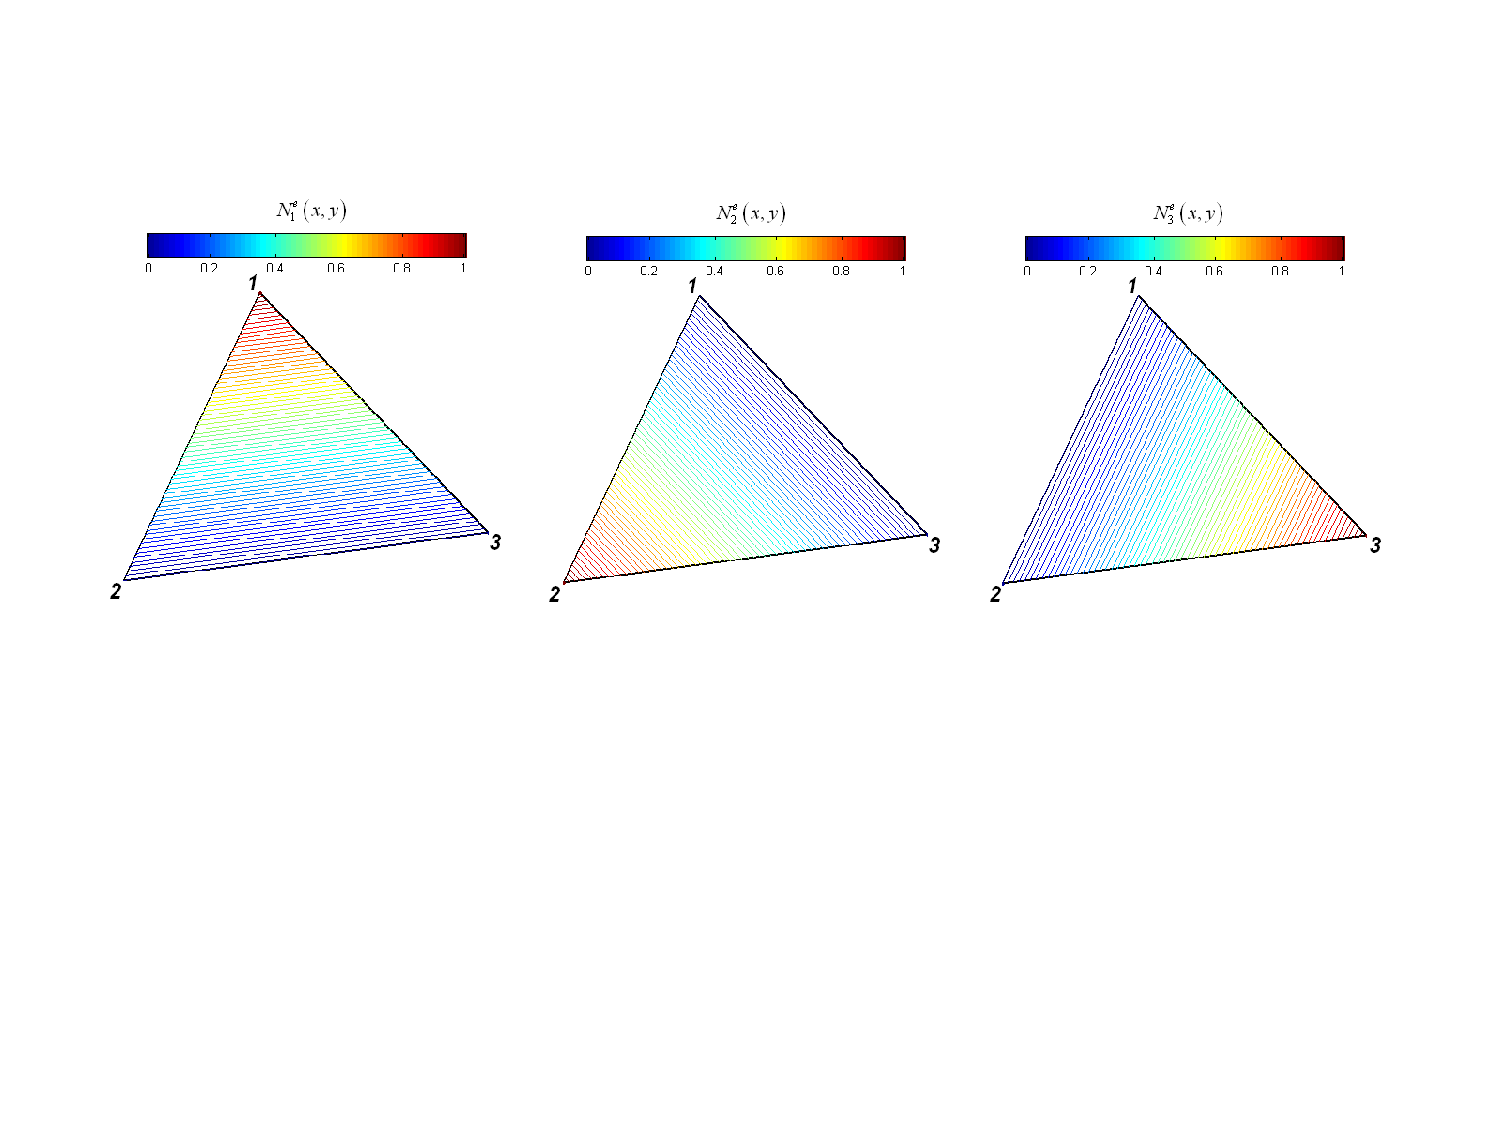
\includegraphics[width=.8\textwidth]{./images/shapeFunc.pdf}
\end{figure}

Due to local character of the shape function, it is simple to switch from the local (element based) notation to the global (computational domain) notation:
\begin{equation*}
	\Phi^e(x,y) = \sum_{i=1}^{3}{N_i}^e(x,y) \cdot {\Phi_i}^e \xrightarrow{\textrm{Local to Global Notation}} \Phi(x,y) = \sum_{i=1}^{N_n} N_i(x,y) \cdot \Phi_i
\end{equation*}

\subsection{Sparse Linear System}
\begin{minipage}[lt]{13cm}
	Galerkin method suggests that the shape functions themselves play a role of the weigthing functions: 
	\begin{equation*}
		w_i(x,y) = N_i(x,y)
	\end{equation*}
	which leads to a linear system 
	\begin{equation*}	
		\left[K\right] \cdot \underbrace{\{\Phi\}}_{\textrm{unknowns}} = \underbrace{\{b\}}_{\textrm{source}}
	\end{equation*}
	It is evident that each element contributes to the matrix and to the right-hand side. 
\end{minipage}
\begin{minipage}[rt]{7cm}
	\begin{centering}
		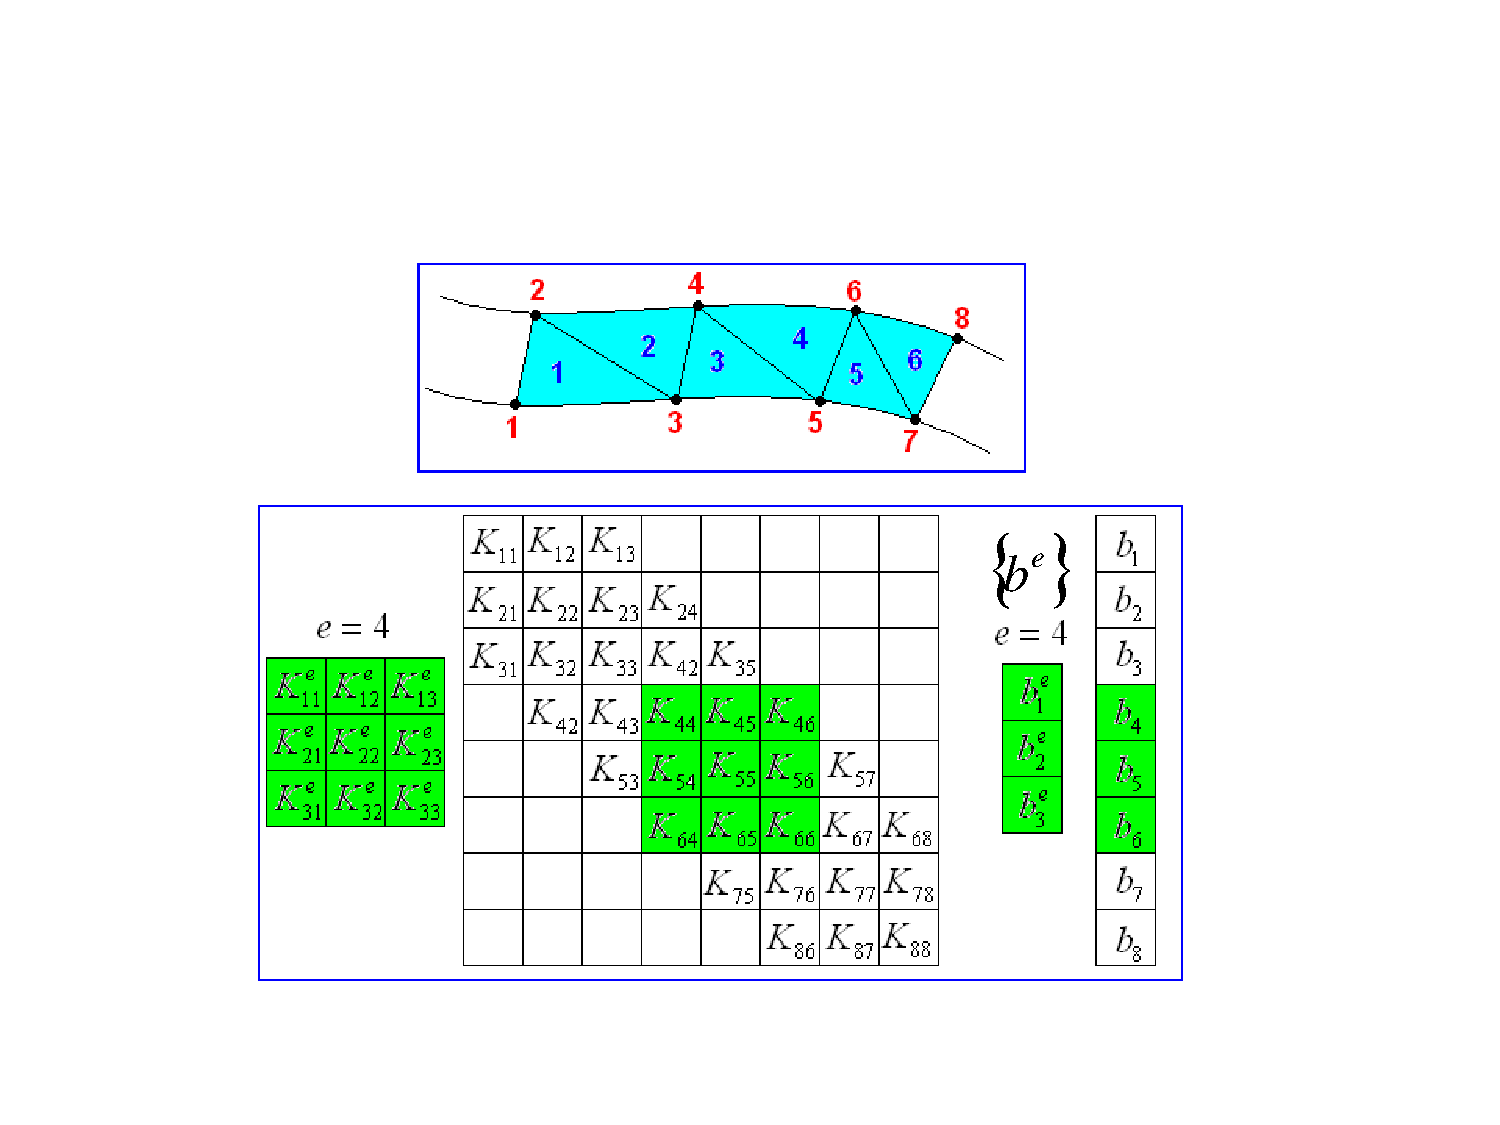
\includegraphics[width=.85\textwidth]{./images/sparse.pdf}
	\end{centering}
\end{minipage}

\textbf{Solvers \\}
Direct solution of the FEM System of equations
\begin{itemize}
	\item LU-decompositon
	\item Cholesky factorization
	\item Direct methods are impractical for large systems (above $10^6$ unknowns) due to ist high number of mathematical operations and round-off error
\end{itemize}
Iterative solution methods
\begin{itemize}
	\item CG
	\item BiCG
	\item GMRES (best for 3D)
	\item Iterative methods are very suitable for large systems but have a slow convergence when the FEM matrix is ill-conditioned (which is usually the case)
	\item Convergence acceleration could be achieved by using preconditioning methods: diagonal preconditioning, ILU (incomplete-LU), ect. 
\end{itemize}
\section{Dielectric Simulations}

Sharp edges, corners or triple points of dielectric and conductive bodies are typical field enhancement regions. \newline
\begin{minipage}[lt]{15cm}
	Following arrangements can limit these enhancements:
	\begin{itemize}
		\item Geometrical rounding of the sharp corners and edges reduces the electric field around them and thus mitigate the dielectric problems.
		\item Shielding, where the shield is on the same potential.
		\item Coating with a high(er) permittivity material. 
		\begin{equation*}
			E_{n,\textrm{coating}} = \frac{\varepsilon_{r,\textrm{conductor}}}{\varepsilon_{r,\textrm{coating}}} \cdot E_{n,\textrm{conductor}}
		\end{equation*}
		\item Hiding triple points to capture the electrons.
	\end{itemize}
\end{minipage}
\begin{minipage}[rt]{4cm}
	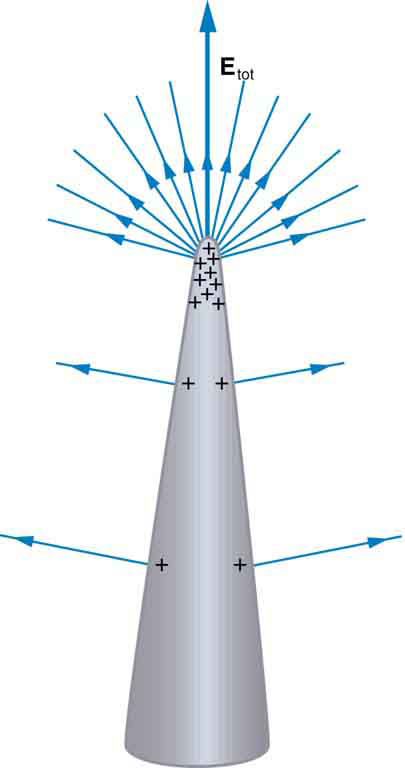
\includegraphics[width=.7\textwidth]{./images/fieldEnhancement.jpeg}
\end{minipage}
\\
\begin{minipage}{5cm}
	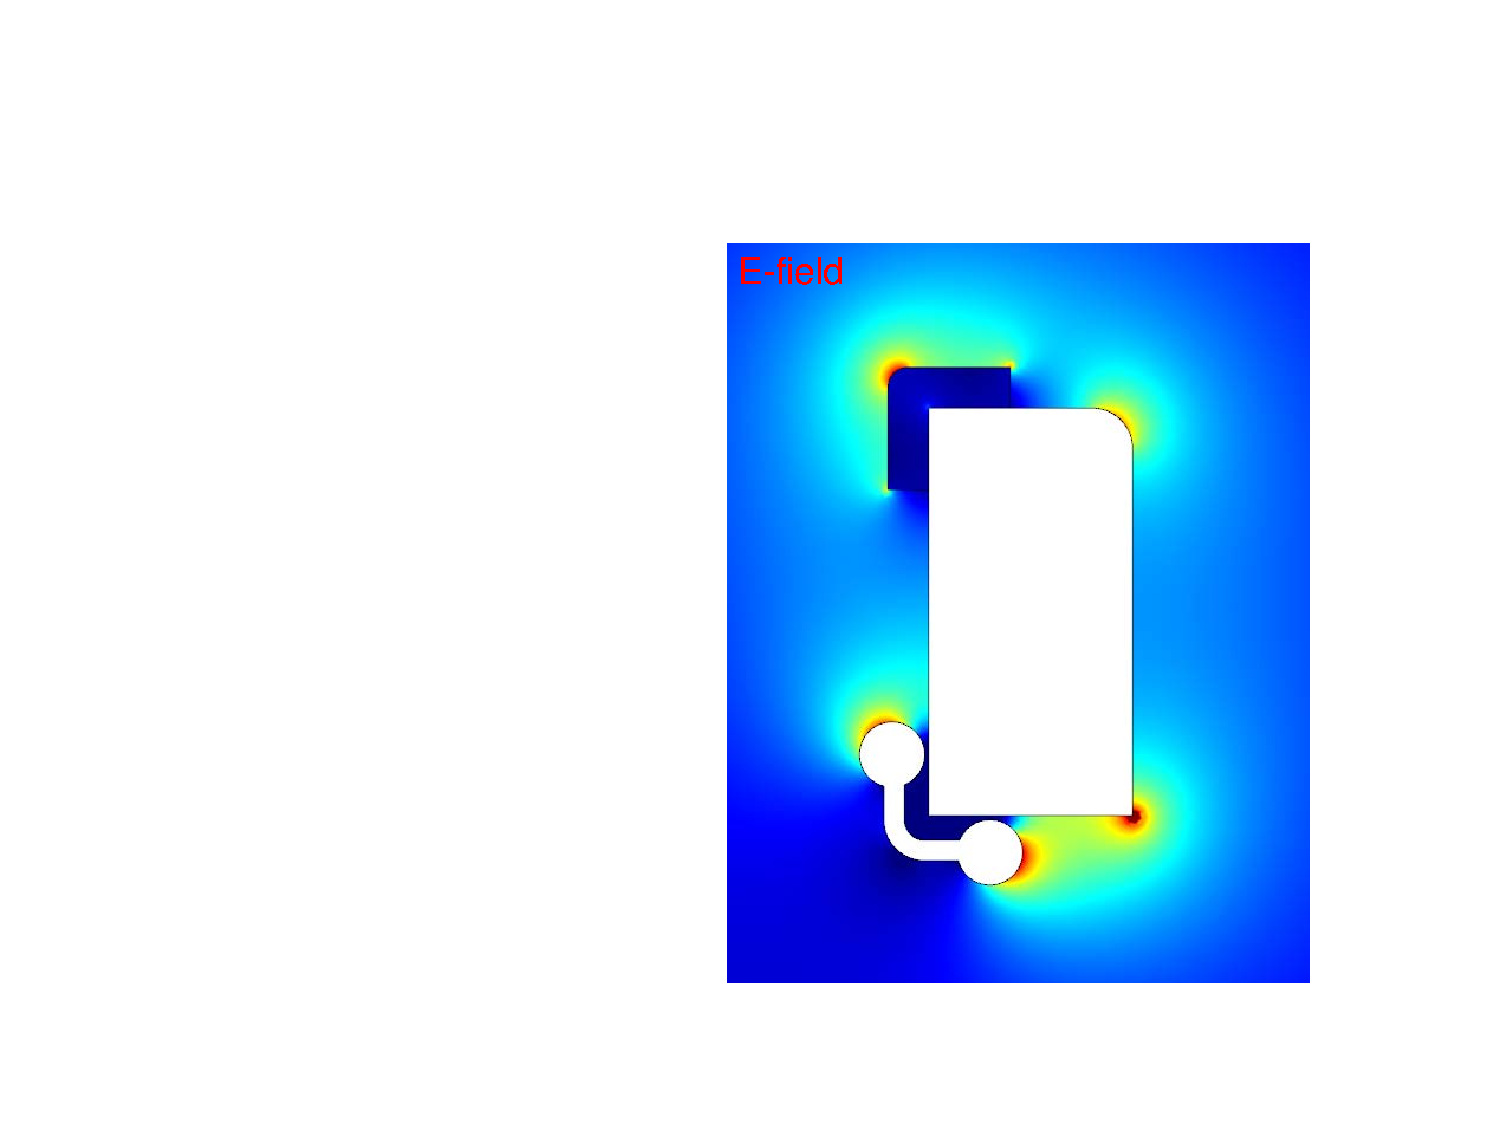
\includegraphics[width=.8\textwidth]{./images/EFields.pdf}
\end{minipage}
\begin{minipage}{7cm}
	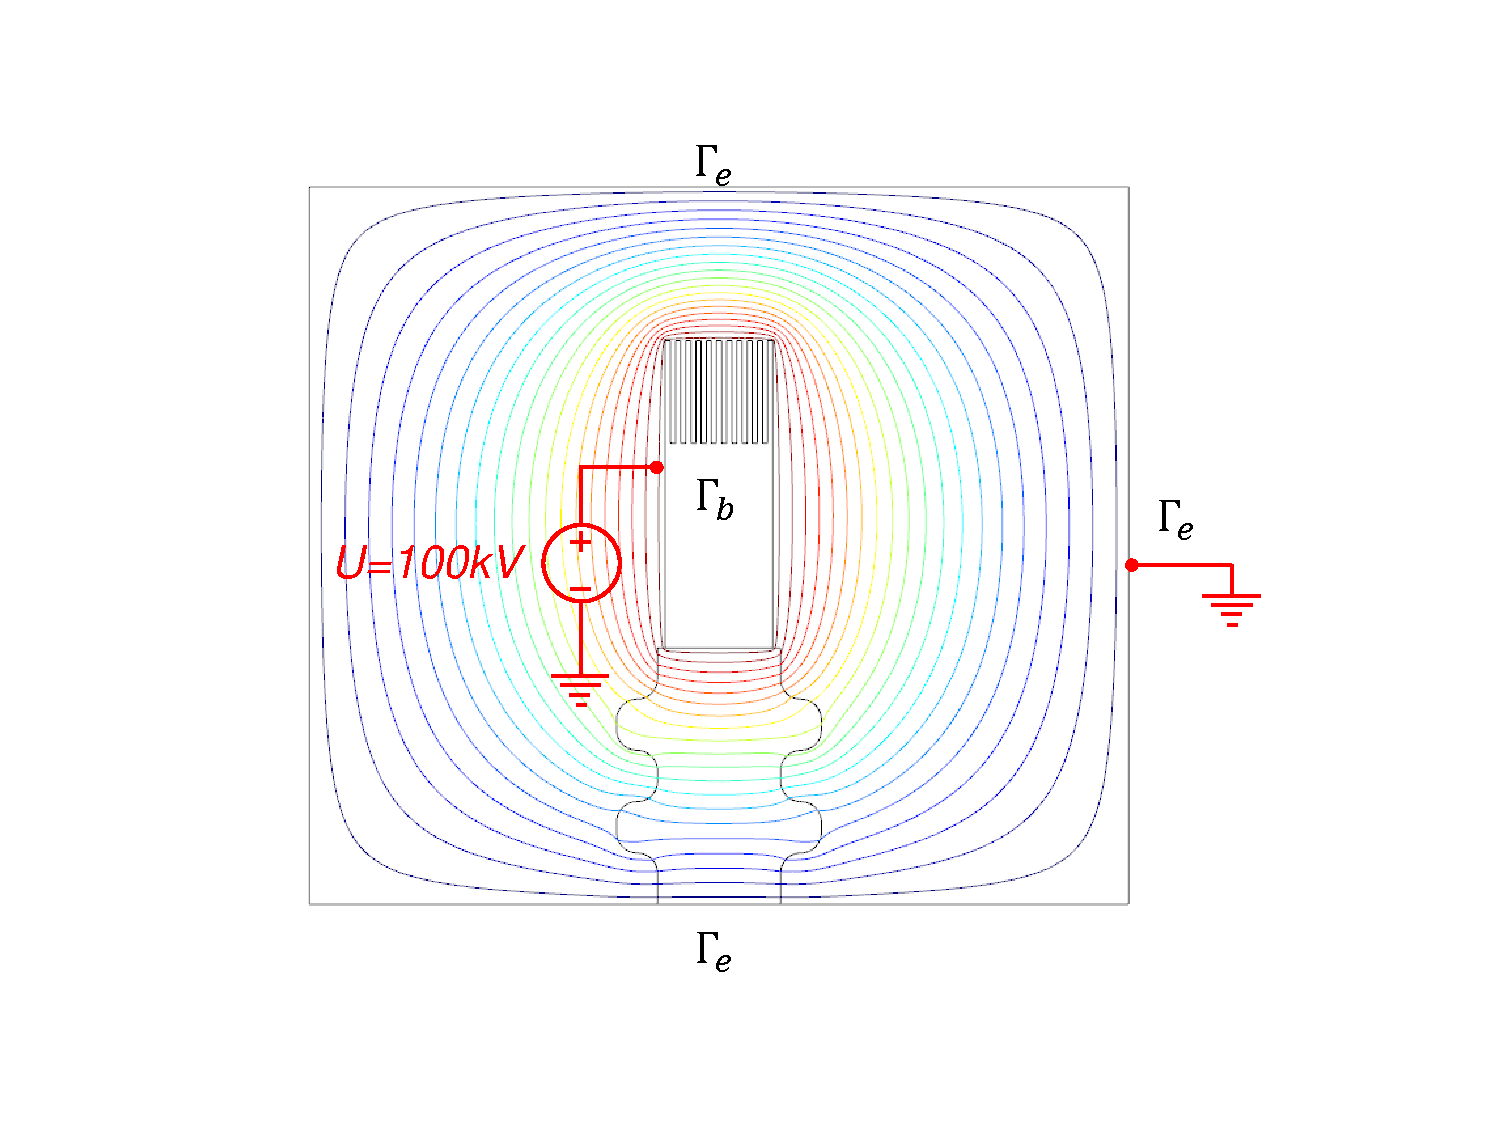
\includegraphics[width=.8\textwidth]{./images/Lines.pdf}
\end{minipage}
\begin{minipage}{7.5cm}
	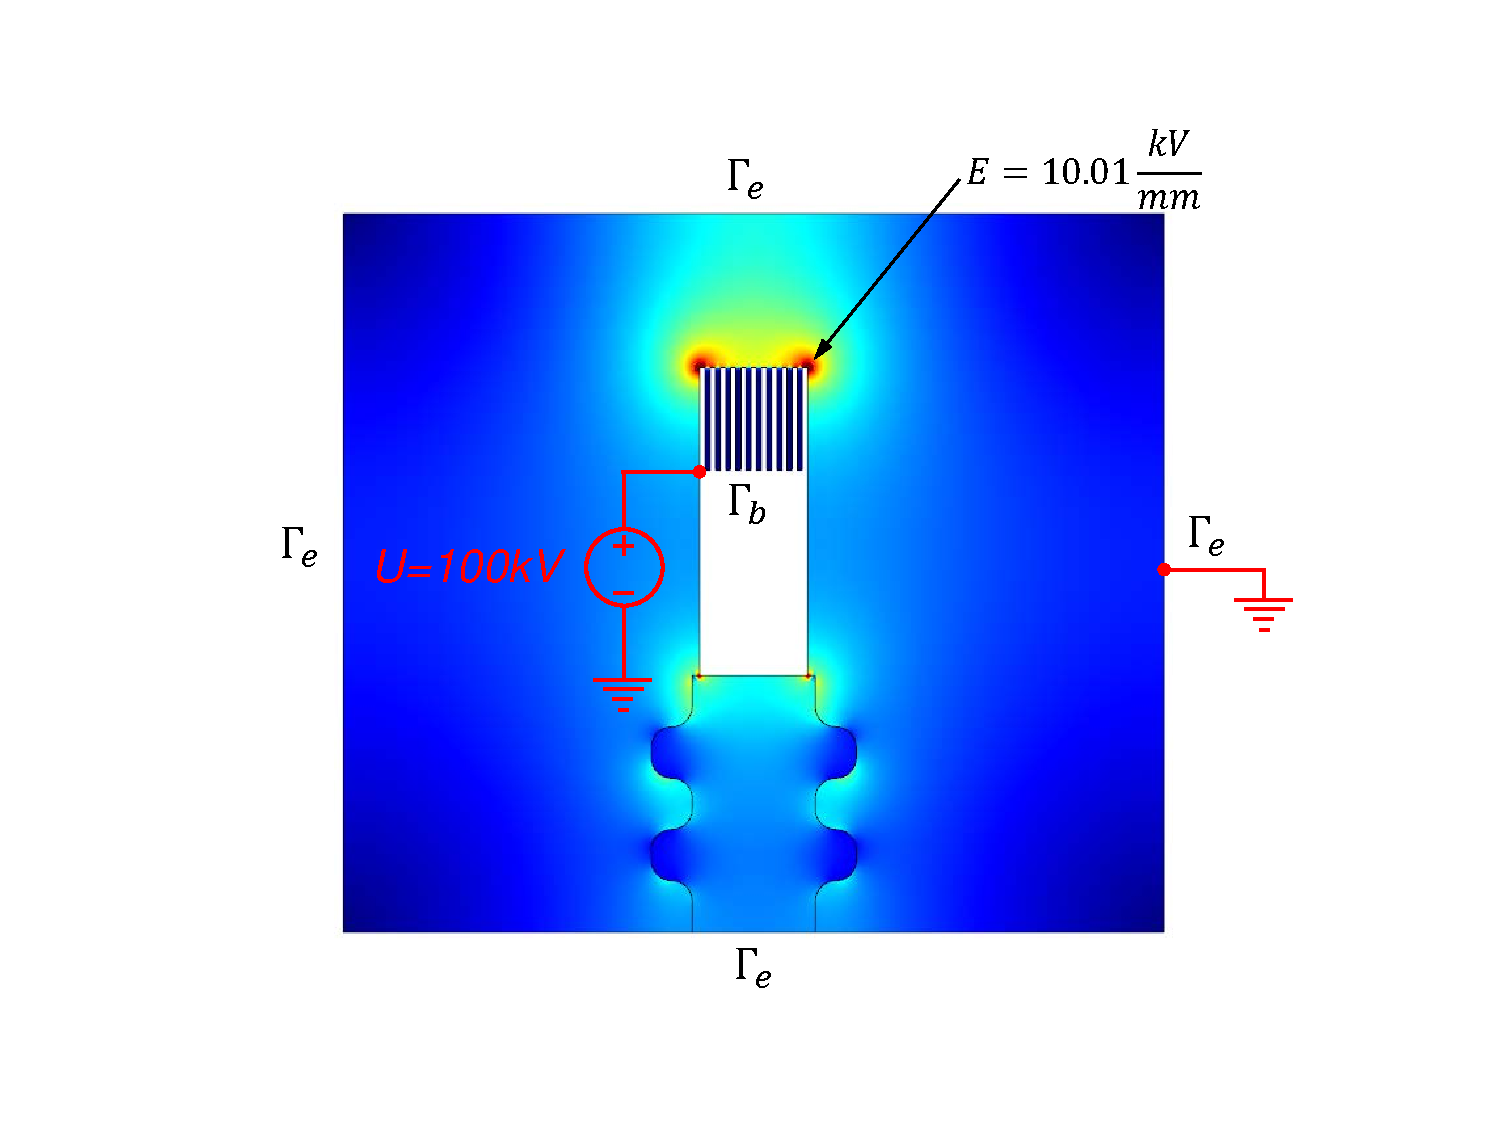
\includegraphics[width=.8\textwidth]{./images/Field.pdf}
\end{minipage}
\section{Eddy Currents}
When an $A_\phi$-Field is going perpendicular through an object, it induces eddy currents. In a transformer this means that the inner LV foil has the highest eddy currents, therefore, it would make sense to make this foil thicker. \newline

Due to skin-effect the current distribution in the LV-foils is non-uniform and can be computed as
\begin{equation*}
	P_\textrm{LV AC} > P_\textrm{LV DC} = R_\textrm{LV DC} \cdot I^2
\end{equation*}

\textbf{\\Shielding \\ \\} 
If there are components made of steel (e.g. a clamp) they can be shielded with copper in order to reduce eddy current. \newline 
\begin{tabular}{ll}
	Steel: 	& \(\displaystyle \mu_r = 150\) \\
			& \(\displaystyle \sigma_{Fe} = 5 \cdot 10^6 \frac{S}{m} \) \\
	Copper: & \(\displaystyle \mu_r 0= 1 \) \\
			& \(\displaystyle \sigma_{Cu} = 5.9 \cdot 10^7 \frac{S}{m} \) \\
\end{tabular} \\ \\
\begin{tabular}{lll}
	 & & Fe:Cu \\
	1. Step: Induced E-field & \(\displaystyle \nabla \times \vec{E} = j\omega\color{red}\mu\color{black}\vec{H} \) & 150:1 \\
	2. Step: Eddy currents  & \(\displaystyle J = \color{red}\sigma\color{black}\vec{E} \) & 1:10 \\
	\textbf{Total:} & & \textbf{15:1}
\end{tabular}\\ \\
$\Rightarrow$ \textbf{15x less eddy current and less losses!}
\newpage
\section{FDTD}
The Finite Difference Time Domain (FDTD) is a method to numerically solve Maxwell equations in time domain, therefore, it is especially suited for transient analysis and/or for wideband analysis. Generally, it is easy to implement and it scales very good for large simulations, however, it is difficult to simulate curved surfaces with this approach.\\
It is not suited for resonant systems or systems with dispersion. But the material properties ($\mu_r,\epsilon_r$) can be set for every computational node separately!\\ 
Mostly very small simulation time steps are required.

\subsection{Numerical Solution of PDEs}
The general Taylor series expansion of function $f(x,t)$ can be written in numerical form as 
\begin{equation*}
	{f_i}^{n+1}= {f_i}^n + \underbrace{\left(t^{n+1} - t^n\right)}_{\Delta t} \frac{\partial f}{\partial t} \bigg\rvert_{i}^{n} + \frac{1}{2} + \underbrace{\left(t^{n+1} - t^n\right)}_{\left(\Delta t\right)^2} \frac{\partial^2f}{\partial t^2} \bigg\rvert_{i}^{n} \Rightarrow \frac{\partial f}{\partial t} \bigg\rvert_{i}^{n} = \frac{{f_i}^{n+1}-{f_i}^n}{\Delta t} - \underbrace{\frac{1}{2}\Delta t \frac{\partial ^2 f}{\partial t^2}\bigg\rvert_{i}^{n}}_{O(\Delta t)} - \dots
\end{equation*}
This approximation is called first order accurate forward difference approximation. \newline Using a sample in the past and a sample in the future it is possible to increase the precision of the approximation but increase the needed memory (residual error scales down with $\Delta t^2$)
\begin{equation*}
	\frac{\partial f}{\partial t} \bigg\rvert_{i}^{n} = \frac{{f_i}^{n+1}-{f_i}^{n-1}}{\Delta t} - \underbrace{\frac{1}{6}\left(\Delta t\right)^2 \frac{\partial ^3 f}{\partial t^3}\bigg\rvert_{i}^{n}}_{O\left[(\Delta t)^2\right]} - \dots
\end{equation*}
Following the same concept, one can calculate the derivative at half-time-steps:
\begin{equation*}
	\frac{\partial f}{\partial t} \bigg\rvert_{i}^{n+\frac{1}{2}} = \frac{{f_i}^{n+1}-{f_i}^{n}}{\Delta t} - \underbrace{\frac{1}{24}\left(\Delta t\right)^2 \frac{\partial ^3 f}{\partial t^3}\bigg\rvert_{i}^{n}}_{O\left[(\Delta t)^2\right]} - \dots
\end{equation*}
With the same approach the second order centered approximation for the spatial derivation can be written as
\begin{equation*}
	\frac{\partial f}{\partial x} \bigg\rvert_{i}^{n} = \frac{{f_{i+1}}^{n}-{f_{i-1}}^{n}}{2\Delta x} - \underbrace{\frac{1}{6}\left(\Delta x\right)^2 \frac{\partial ^3 f}{\partial x^3}\bigg\rvert_{i}^{n}}_{O\left[(\Delta x)^2\right]} - \dots
\end{equation*}

\subsection{Interlieved Leapfrog (lossless transmission line in this case)}
\begin{minipage}[rt]{9cm}
	\begin{tabular}{l}
		By discretising the voltage at integer grid points\\ (centered at $n+1/2,i$), whilst the current at half grid \\points (centered at $n,i+1/2$): \\
		\begin{equation*}
			V_{i}^{n+1} = V_{i}^{n} - \left(\frac{\Delta t}{C \Delta x}\right) \left[I_{i+1/2}^{n+1/2} - I_{i-1/2}^{n+1/2}\right]
		\end{equation*} \\
		\begin{equation*}
			I_{i+1/2}^{n+1/2} = I_{i+1/2}^{n-1/2} - \left(\frac{\Delta t}{L \Delta x}\right) \left[V_{i+1}^{n} - V_{i}^{n}\right]
		\end{equation*} \\
		Stability for 1D Leapfrog (CFL): \\
		\begin{equation*}
			\Delta t \leq \frac{\Delta x}{|v_p|} \textrm{ where } v_p = \frac{1}{\sqrt{LC}} = \frac{c_0}{\sqrt{\epsilon_r\mu_r}}
		\end{equation*} \\
		General stability (CFL) for dimension $D$ \\if $\Delta x = \Delta y = \Delta z$: \\
		\begin{equation*}
			\Delta t \leq \frac{\Delta x}{\sqrt{\varepsilon \mu}} \cdot \frac{1}{\sqrt{D}} = \frac{\Delta x}{v_p} \cdot \frac{1}{\sqrt{D}}
		\end{equation*}
	\end{tabular}
\end{minipage}
\begin{minipage}[rt]{10cm}
	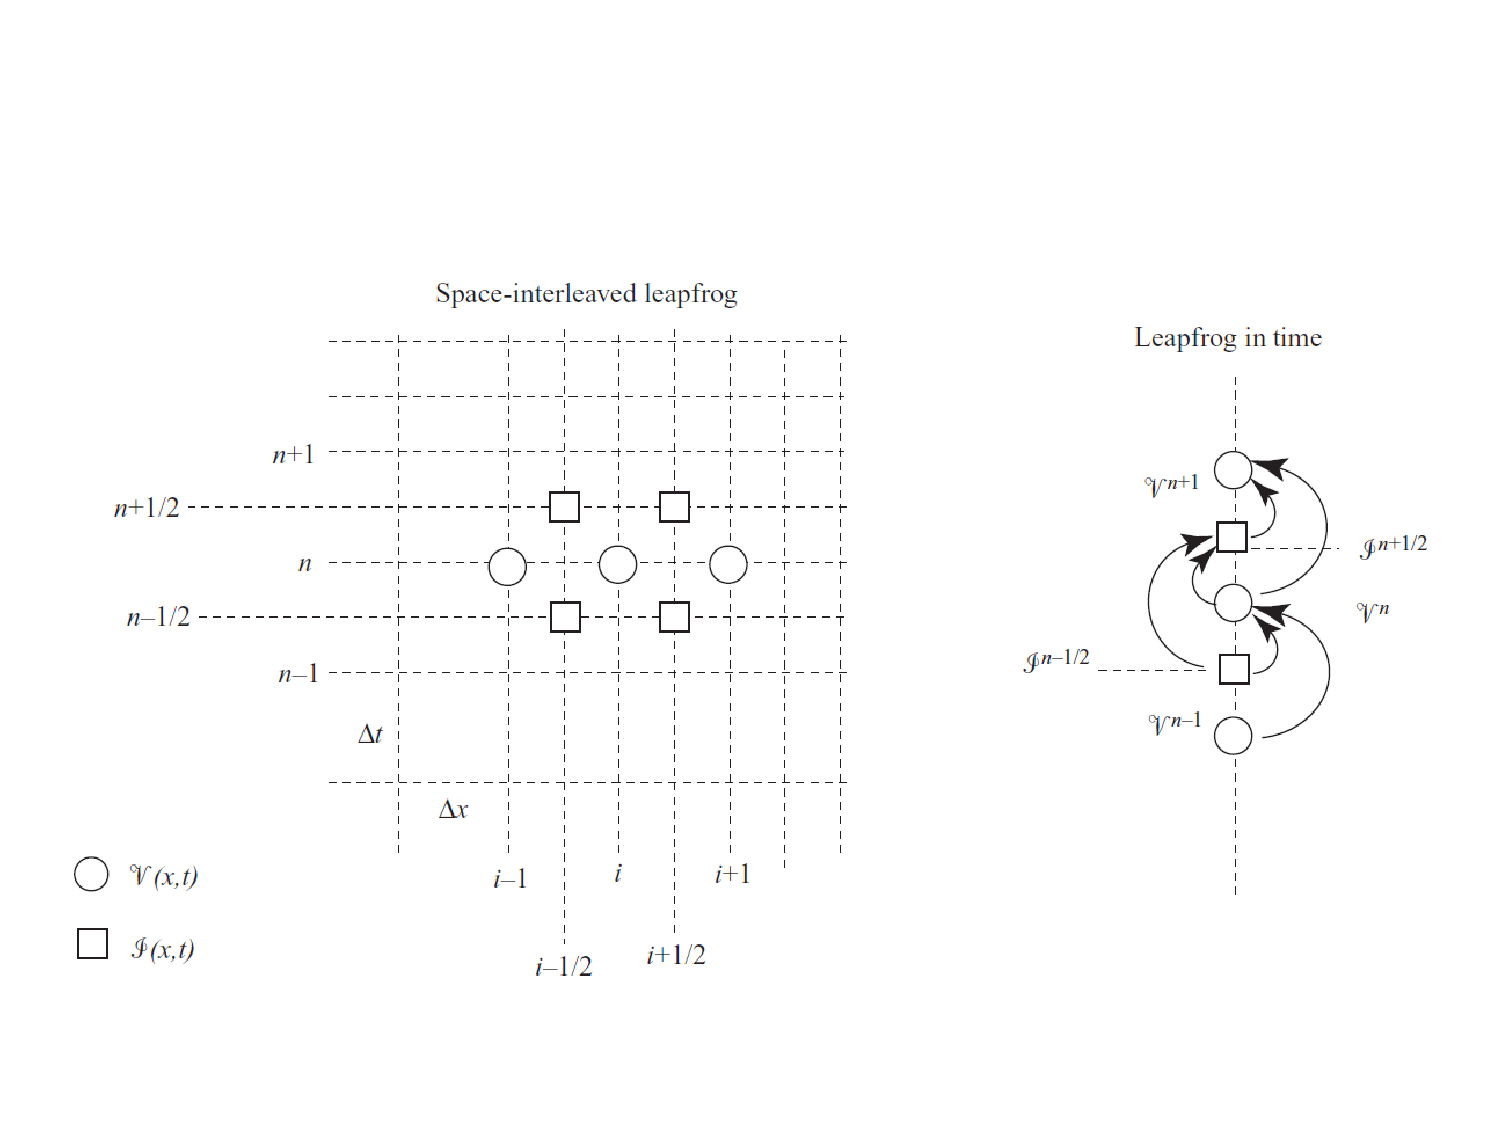
\includegraphics[width=.95\textwidth]{./images/leapfrog.pdf}
\end{minipage}

\subsection{3D Derivation}
\begin{minipage}{12cm}
	The Yee Cell is organized in such a way: \\
	\begin{itemize}
		\item The origin of each cell defines the generic point (i.e. $i,j,k$) at which all vectors are referred to.
		\item The specific component of the electric field is always defined on the \textbf{edges} of the cell containing the origin, displaced by ½ position.
		\item The specific component of the magnetic field is always defined on the \textbf{face} of the cell containing the origin, exactly in the middle.
	\end{itemize}
	Advantages of using the Yee Grid: \\
	\begin{itemize}
		\item Curl equations are automatically satisfied
		\item When considering source free media and second order centered differencing, it can be shown that the Yee cell guaraties divergence difference equations \(\displaystyle \left(\nabla \cdot \vec{B} = 0 \textrm{ (always true)}, \nabla \cdot \vec{E} = 0 \textrm{ (normally true)} \right)\) 
		\item Boundary donditions are automatically satisfied
	\end{itemize}
\end{minipage}
\begin{minipage}{7cm}
	\begin{flushright}
	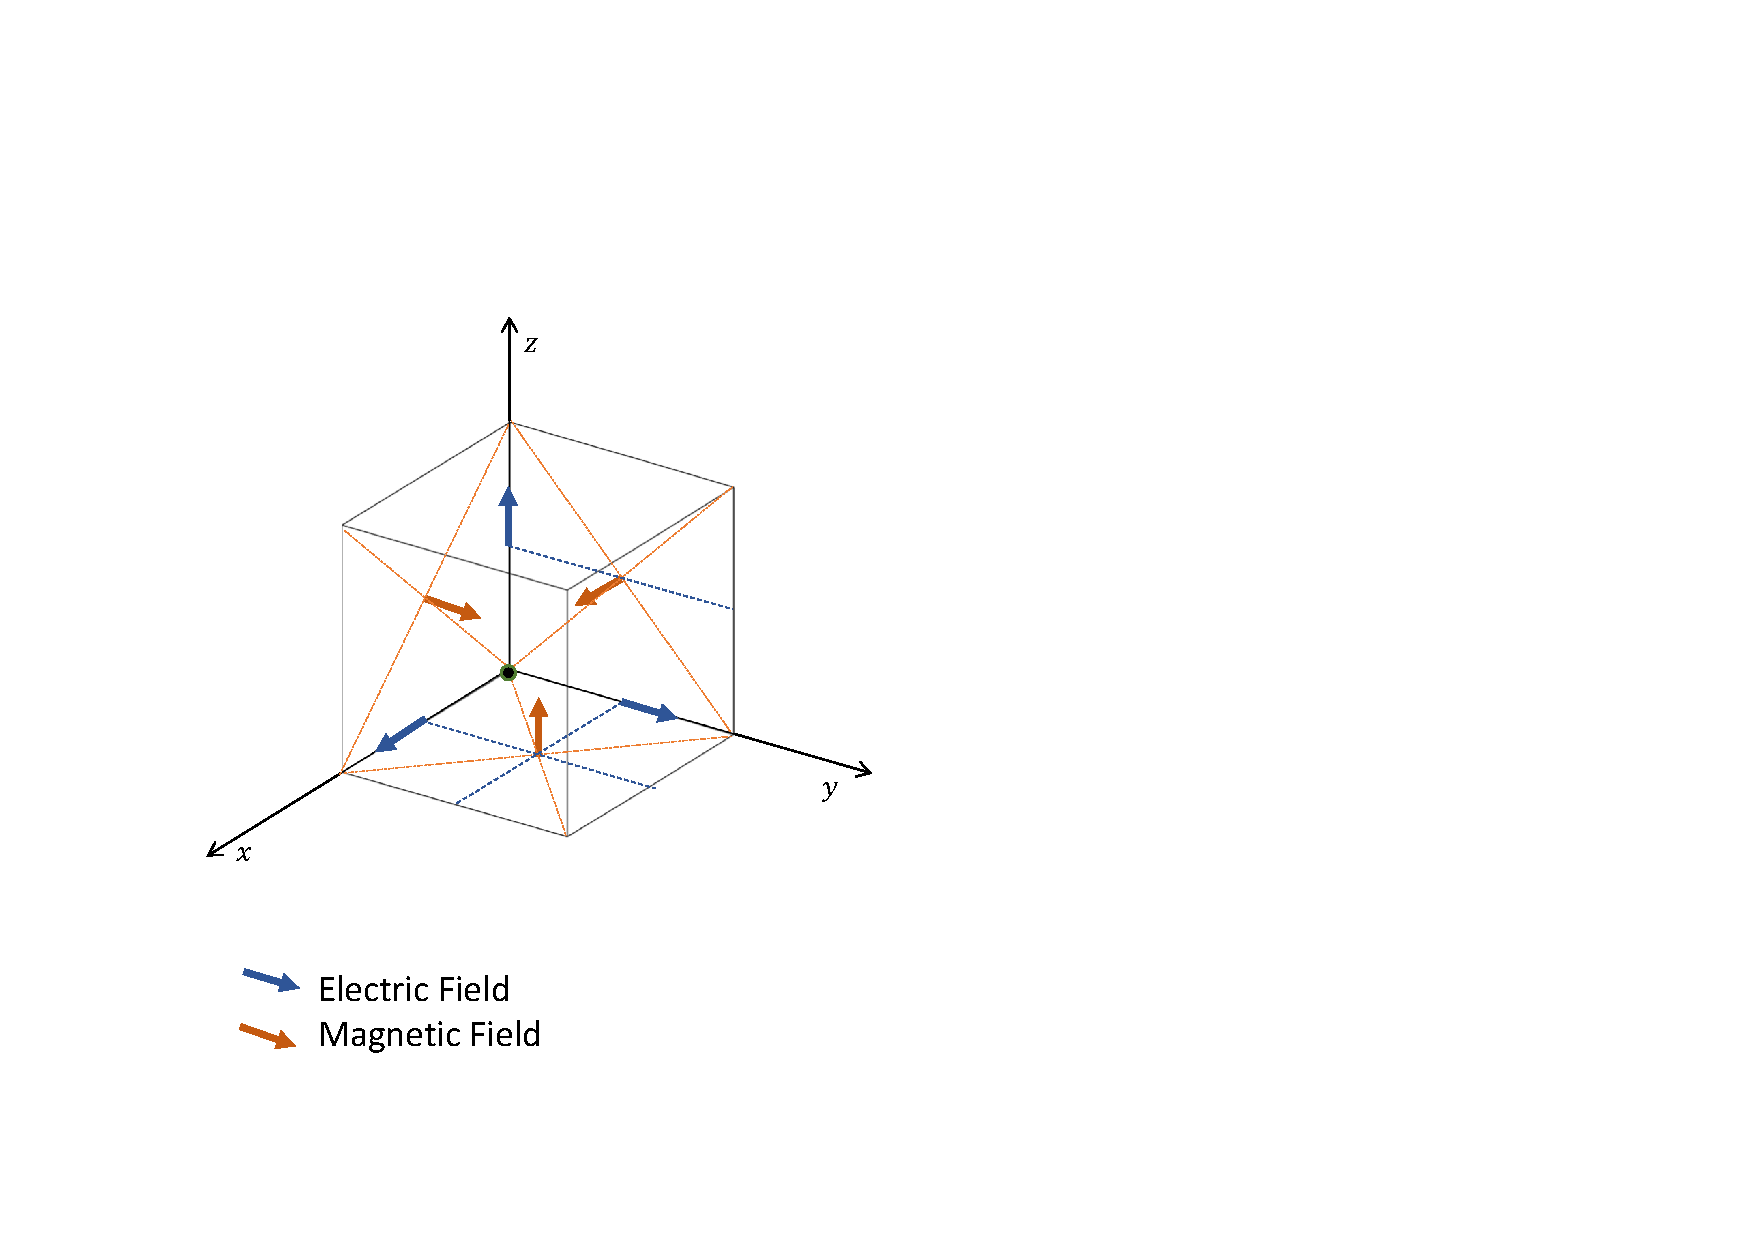
\includegraphics[width=.95\textwidth]{./images/Yee.pdf}
	\end{flushright}
\end{minipage}

\subsection{Normalization of H}
In free space Electric and Magnetic field are related through the characteristic impedance $Z_0$ of free space with
\begin{equation*}
	Z_0 = \frac{E}{H}=\sqrt{\frac{\mu_0}{\varepsilon_0}} \approx 120\pi~\Omega \approx 377~\Omega.
\end{equation*}
This means that the amplitude of the electric field is always at least 377 times bigger than the one of the magnetic field. In order to have a better numeric approximation is common practice to normalize the magnetic field vector using the following expression
\begin{equation*}
	^*\overline{H} = \sqrt{\frac{\mu_0}{\varepsilon_0}} \overline{H}.
\end{equation*}

\subsection{Choice of the time and spatial step}
\label{sec:steps}
The choice of time step is driven by the spatial step and CFL condition. Assuming in general  $\Delta x = \Delta y = \Delta z$ 
\begin{equation*}
	\Delta t \leq \frac{\Delta x}{|v_p|} \cdot \frac{1}{\sqrt{D}}
\end{equation*}
If $\Delta x \neq \Delta y \neq \Delta z$ the following formula should be used:
\begin{equation*}
	\Delta t \leq \frac{1}{|v_p|} \cdot \frac{1}{\sqrt{\Delta x^2+\Delta y^2+\Delta z^2}}
\end{equation*}
the choice of the spatial step is provided by 
\begin{equation*}
	\Delta x \leq \frac{1}{m_\textrm{ovs}} \min (\lambda_\textrm{min},d_\textrm{min})
\end{equation*}
where $m_\textrm{ovs}$ represents the oversampling ratio in spatial domain. Typical values for $m_\textrm{ovs}$ are between 10 and 100. $\lambda_\textrm{min}$ is the smallest wavelength in our system. Generally it is defined as 
\begin{equation*}
	\lambda_\textrm{min} = \frac{v_p}{f_\textrm{max}} = \frac{c_0}{\sqrt{\varepsilon_{r,\textrm{min}}\mu_{r,\textrm{min}}}\cdot f_\textrm{max} }
\end{equation*}
where $v_p$ is the smallest velocity of the wave in any medium of our system, $d_\textrm{min}$ represents the smallest feature dimension we need to simulate and $f_\textrm{max}$ is the maximum frequency of the stimulus.

\subsection{Implementation in MATLAB (1D-FDTD Algorithm)}
How to implement 1D-Maxwell wave equations in MATLAB:\\
\begin{tabular}{l}
	\textbf{1. Initialize E and H vectors to zero}\\
	\includegraphics[width=.6\textwidth]{./images/InitVectors.pdf}\\
	The update coefficients are expressed to calculate *H directly\\
	\textbf{2. Setup time and spatial step}\\
	See chapter \ref{sec:steps}.
	Feature and time steps can only be expressed in integer numbers!! $\rightarrow$ ceil()\\
	\textbf{3. For each time step}\\
	\begin{tabular}{l}
		\hspace{1cm}Setup sources\\
		\hspace{1cm}for each spatial step\\
		\hspace{2cm}update the magnetic field from the electric field\\
		\hspace{2cm} \includegraphics[width=.5\textwidth]{./images/updateH.pdf}\\
		\hspace{2cm}end update H\\
		\hspace{1cm}Setup boundary conditions on H\\
		\hspace{1cm}for each spatial step\\
		\hspace{2cm}update the magnetic field from the electric field\\
		\hspace{2cm} \includegraphics[width=.5\textwidth]{./images/updateE.pdf}\\
		\hspace{2cm}end update H\\
		\hspace{1cm}Setup boundary conditions on H\\
	\end{tabular}
	\\
	\textbf{4.	End loop in time}
\end{tabular}

\subsubsection{Boundary conditions for waves}
\begin{itemize}
	\item \textbf{Total Reflectiong Condition:} The E-Field is set to zero outside the grid. The energy is kept in the grid and bounced back and forth. This assignment is equivalent to the Perfect Electric Conductor (PEC) boundary.\\
	$E(first)=0 \hspace{1cm} E(last) = 0$\\
	Not very useful because there is no PEC existing in nature and the energy remains in the grid what is illogical as well.
	\item \textbf{Periodic Boundary Condition}: Is used for periodic structures. A structures periodicity is reflected in the same periodicity of the E- and H-field.\\
	\begin{minipage}{12cm}
		$E_{first}(Cell 2)=E_{Last}(Cell1)$ \hspace{1cm}and\hspace{1cm} $E_{Last}(Cell 1)=E_{first}(Cell2)$ \\ \\
		And in MATLAB:\\
		\includegraphics[width=0.5\textwidth]{./images/periodic_MATLAB.pdf}\\
		\textbf{Attention!!} $E(1)$ and $E(kStep+1)= E(last)$ are not allowed to be updated
	\end{minipage}
	\begin{minipage}{7cm}
		\begin{flushright}
			\includegraphics[width=1\textwidth]{./images/periodic.pdf}\\
		\end{flushright}
	\end{minipage}
	
	\item \textbf{Absorbing Boundary Condition}: The incident wave will travel through the boundary without reflection. This is specially used at the bounding box. The solution will then be similar as when the bounding box has infinite size $\rightarrow$ smaller bounding boxes can be used.\\
	The Mur boundary is a special absorbing boundary where the wave is artificially cancelled out. Eliminating forward travelling waves: 
	\begin{equation}
	E^{n+1}_1 = E^n_2 - \frac{1-\alpha}{1 + \alpha} \cdot (E^{n+1}_2 + E^n_1 )
	\end{equation}
	Eliminating backward travelling waves:
	\begin{equation}
		E^{n+1}_{last} = E^n_{last-1} - \frac{1-\alpha}{1 + \alpha} \cdot (E^{n+1}_{last-1} + E^n_{last} )
	\end{equation}
	where $\alpha$ is:
	\begin{equation}
		\alpha = \frac{\Delta t}{\Delta z}\cdot c_0
	\end{equation}
	These are the Mur boundary conditions for 1D. \\2D and 3D is much more complicate and Mur boundaries are not suitable. There we use Perfect Matched Layer Boundaries (PMC).
\end{itemize}

\subsubsection{Sources}
A source can be an electric, a magnetic field or a current source. In the last case, the curl equation including the displacement current must be used.
\begin{itemize}
	\item \textbf{Hard Sources}: The source is hardly introduced at specific position in space and the value of the field is substituted (overwritten) with the source value. This is often very useful to modelling antennas because the source appears to the wave like a PEC boundary:\\ \\
	$E_x(SourceZUsed) = src;$
	\\
	\item \textbf{Soft Sources}: The source is superimposed to the field value at a specific position in space. If a wave comes back its value is added to the value of the source. Useful when modelling scattered structures but not ideal because the source sends energy in all directions.\\ \\
	$E_x(SourceZUsed) = E_x(SourceZUsed)+src;$\\
	\item \textbf{TF/SF Source}: This is a kind of soft source called Total Field/Scattered Field source.
	This source has the advantage to travel only in one direction and is transparent for the scattered wave. To implement this, the space is divided in a region where all fields are available (Total Field) and a region where just the scattered field is available.\\This can be achieved by updating the E and H-equations with an additional term:\\ \\
	$E_x(SourceZUsed) = E_x(SourceZUsed)+UC_Ex(SourceZUsed)*src;$\\
	$H_y(SourceZUsed) = H_y(SourceZUsed)+UC_Hy(SourceZUsed)*src;$\\
\end{itemize}


\newpage
\section{RF Antennas}
Generally, an antenna is a system which allows to couple electromagnetic energy from a circuit into free space. It uses the benefit that an oscillating magnetic field generates an oscillating electric field and vise versa.

\subsection{Antenna Parameters}

\begin{minipage}{10cm}
\begin{itemize}
	\item \textbf{Impedance Matching:} To transfer the maximum energy from the transmission line over the antenna to free space folowing condition should be satisfied:
	\begin{equation}
	Z_{ant} = Z^*_{TL} 
	\end{equation}
	\item \textbf{Radiation Pattern:} Defines how the electromagnetic energy radiated by the antenna is spatially distributed in free space. (Doughnut plots)\\ It is the normalized radiation intensity in a polar plot. It is usually given in dB: \\
	$F_{dB}(\phi,\theta)=10log_{10}F(\phi,\theta)$
	\item \textbf{Radiation Efficiency:} Defines the ratio between the radiated energy and the energy applied to the antenna system.
	\item \textbf{Bandwidth:} Usually, the bandwidth is defined as the frequency range where the radiated power is up to 10dB below the maximum radiated power ( $1<\textrm{VSWR}<1.5$)
	\item \textbf{Near Field:} $\lambda < r < 4$	\hspace{2cm} \textbf{Far Field:} $ r > 10\cdot \lambda$
	\item \textbf{Reciprocity:} An antenna receives signals as good as it can transmit them.

\end{itemize}
\end{minipage}
\begin{minipage}{8cm}
	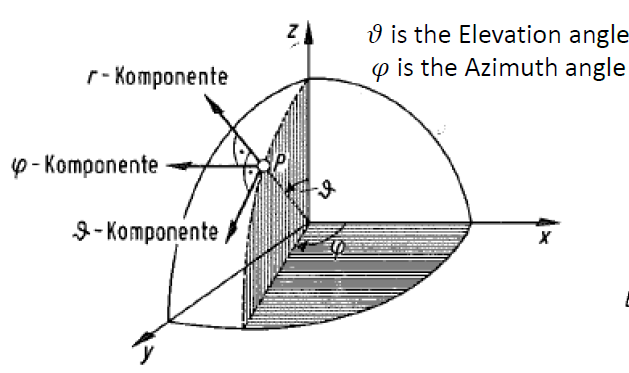
\includegraphics[width=1\textwidth]{./images/Antenna_Pattern.png}\\
\end{minipage}

\begin{tabular}{|l|c|c|}
	\hline \textbf{Description} & \textbf{Equation} & \textbf{Hertzian Dipole}\\
	\hline Impedance of free space (Far field only) & $Z_0 =\frac{E_\theta}{H_\phi} = \sqrt{\frac{\mu_0}{\varepsilon_0}} \approx 377 \Omega$ & \\
	\hline Time averaged radiated Power & $S(r,\phi,\theta)=\int_{0}^{T}\vec{E}\hspace{0.1cm} x\hspace{0.1cm} \vec{H}dt $ & $Z_0 \frac{I_0^2}{8r^2}(\frac{d}{\lambda})^2 \hspace{0.1cm} sin^2 \theta$ \\
	\hline Total radiated Power & $ P_s=\int_{\phi}^{}\int_{\theta}^{}S(r,\phi,\theta)\cdot r^2 sin\theta \hspace{0.1cm} d\theta\hspace{0.1cm} d\phi$ & $Z_0 I_0^2 \frac{\pi}{12}(\frac{d}{\lambda})^2$   \\
	\hline Normalized Radiation Intensity & $ F(\phi,\theta)=\frac{S(r,\phi,\theta)}{max[S(r,\phi,\theta)]}$ & $sin^2 \theta$\\
	\hline Power density of Isotropic Antenna (fictional) & $ S_i = \frac{P_s}{4\pi r^2}$ & \\
	\hline Directivity (in a preferred direction) & $ D = \frac{max[S(r,\phi,\theta)]}{S_i}$ & $\approx 1.5 $ depends on the length\\
	\hline Radiation Resistance & $ R_{rad} = \frac{2P_{rad}}{I_0^2}$ & \\
	\hline Radiation Power & $ P_{rad} = 0.5 \cdot I_0^2 \cdot R_{rad} $ & \\ 
	\hline Antenna (ohmic) losses & $ P_{loss} = 0.5 \cdot I_0^2 \cdot R_{loss} $ & \\ 
	\hline Radiation Efficiency & $ \eta = \frac{P_{rad}}{P_{P_tot}}$ & \\
	\hline Antenna Gain & $G = \eta \cdot D $ & \\
	\hline Equivalent Isotropic Radiated Power & $EIRP = G \cdot P_s$ & \\
	\hline Antenna Impedance & $ Z_{ant} = R_{loss}+R{rad} +jX $ & \\
	\hline Reflection Factor & $\Gamma = \frac{Z_{Ant}- Z_{TL}}{Z_{Ant} + Z_{TL}}$ & \\
	\hline Voltage Standing Wave Ratio & $ \textrm{VSWR} = \frac{1+\Gamma}{1-\Gamma} > 1$ & \\
	\hline Effective Antenna Area & $ A_{eff,RX} = \frac{P_{RX}}{S(r,\phi,\theta)} = \frac{\lambda^2 D_{RX}}{4\pi} $ & \\
	\hline Ratio between transmitted and received power & $ P_{RX} = P_{TX}\cdot G_{TX}\cdot G_{RX}\cdot (\frac{\lambda}{4 \pi R})^2 $ & R = Distance between Antennas\\
	\hline Free Space Path Loss & $ \textrm{FSPL} = 20log_{10} \frac{4\pi R}{\lambda}$ & $\lambda = \frac{c}{f}$ \\
	\hline 
\end{tabular} 



\newpage
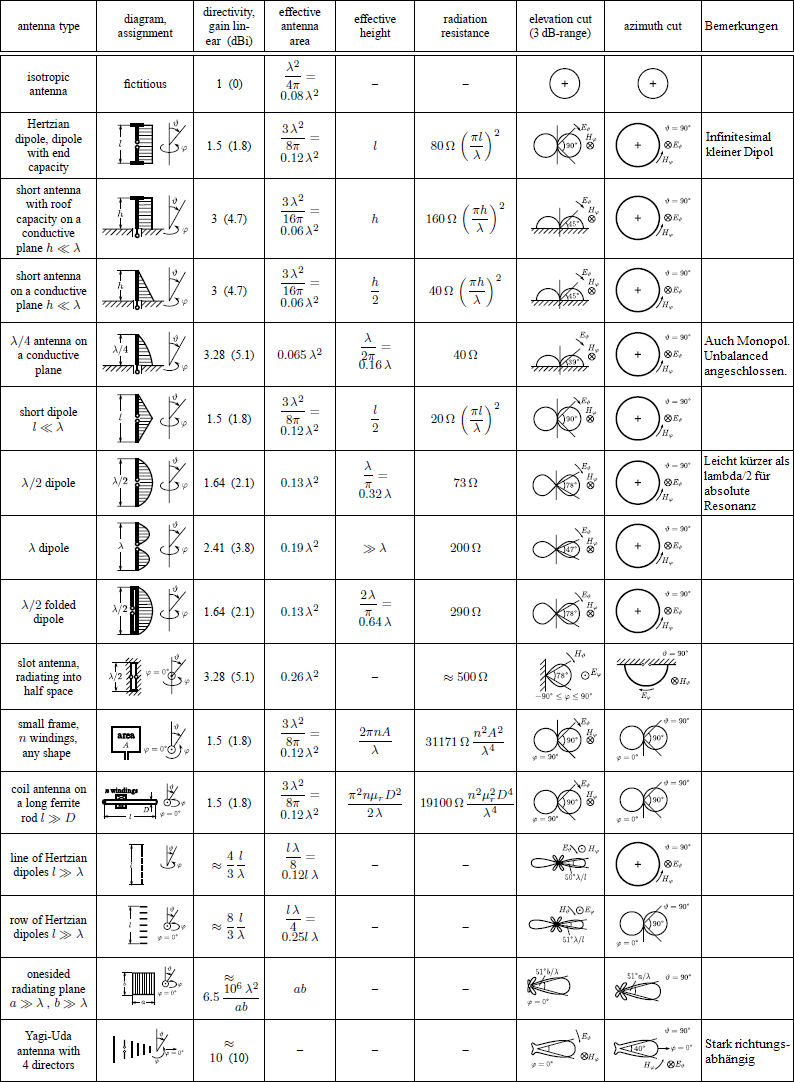
\includegraphics[width=1\textwidth]{./images/antennas-overview.png}\\
\section{Transmission Lines}
A transmission line is a special structure designed to guide waves. The waves are guided in a dielectric by means of reflections between the conductors.

\begin{itemize}
	\item TEM Modes: The direction of propagation is orthogonal to the direction of electric and magnetic field.
	\item TE Modes: The direction of propagation is normal to the E-field but not H-field.
	\item TM Modes: The direction of propagation is normal to the H-field but not E-field.
\end{itemize}


\subsection{Transmission Line Equations}
\begin{tabular}{p{8cm}p{4.5cm}p{5cm}}
	\begin{minipage}{8cm}
		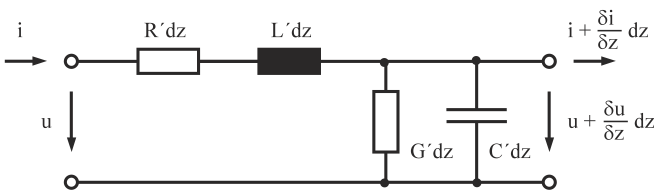
\includegraphics[width=8cm]{./images/LeitungselementESB.png}
	\end{minipage}&
	\begin{minipage}{4.5cm}
		\textbf{Distributed Parameters}\\
		$R'[\frac{\Omega}{m}]: \text{Resistance}$\\
		$L'[\frac{H}{m}]: \text{Inductance}$\\
		$G'[\frac{S}{m}]: \text{Conductance}$\\
		$C'[\frac{F}{m}]: \text{Capacity}$\\
	\end{minipage}&
	\begin{minipage}{5cm}
		\textbf{No Load}:\\
		$\underline{Y}_L=\frac{1}{\underline{Z}_L}=\frac{\underline{I}_L}
		{U} = G+j\omega C=\frac{\alpha l+j\beta l}{\underline{Z}_W}$\\
		\textbf{Short Circuit}:\\
		$\underline{Z_K}=\frac{U}{\underline{I}_K} = R+j\omega
		L=(\alpha l+j\beta l)\underline{Z}_W$\\
	\end{minipage}\\
	\begin{minipage}{8cm}
		\vspace{0.3cm}
		$\underline{U}_1=\cosh(\gamma l)\cdot \underline{U}_2+
		\underline{Z}_W \cdot \sinh(\gamma l)\cdot \underline{I}_2$\\
		$\underline{I}_1=\frac{1}{\underline{Z}_W}\cdot \sinh(\gamma l)\cdot
		\underline{U}_2+ \cosh(\gamma l)\cdot \underline{I}_2$  	
	\end{minipage} &
	\begin{minipage}{9cm}
		\vspace{0.3cm}
		$\begin{bmatrix}
		\underline{U}_1\\
		\underline{I}_1
		\end{bmatrix}=
		\begin{bmatrix}
		cosh(\gamma l) & \underline{Z}_W sinh(\gamma l)\\
		\frac{1}{\underline{Z}_W}sinh(\gamma l) & cosh(\gamma l)
		\end{bmatrix} \cdot
		\begin{bmatrix}
		\underline{U}_2\\
		\underline{I}_2
		\end{bmatrix}$\\
	\end{minipage}
\end{tabular}\\
if $\alpha l >> \beta l$ then $cosh(\gamma l)\approx sinh(\gamma
l)=\frac{1}{2} e^{\gamma l}$ !!!

\subsubsection{Lossy Transmission Lines}
\renewcommand{\arraystretch}{1.5}
\begin{tabular}{| p{7.7cm} | l |}
	\hline
	\textbf{Propagation Factor}
	& $\gamma=\alpha+j\beta=\sqrt{(R'+j\omega L')(G'+j\omega C')}\qquad
	\alpha=[\frac{Np}{m}] \qquad \beta=[\frac{^\circ}{m}]$\\
	\hline
	\textbf{Damping Constant}
	& $\alpha l= \frac{1}{2}ln(Re\{e^{2\gamma l}\})=\alpha\cdot l$\\
	\hline
	\textbf{Phase Delay}
	& $\beta l=\frac{1}{2}ln(Im\{e^{2\gamma l}\})= \beta\cdot l$ \qquad
	$\beta=\frac{\omega}{v_P}$\\
	\hline
	\textbf{Characteristic Impedance}
	& $\underline{Z}_W=\frac{\underline{U}}{\underline{I}}=\sqrt{\frac{R'+j\omega L'}{G'+j\omega C'}}$
	$=\sqrt{\underline{Z}_L \cdot \underline{Z}_K}$\\
	\hline
	\textbf{Input Imp. $\underline{Z}_1$  with termination $\underline{Z}_a$} &
	$\underline{Z}_1 = \underline{Z}_W
	\frac{\underline{Z}_a+\underline{Z}_W \cdot \tanh(\gamma
		l)}{\underline{Z}_W+\underline{Z}_a \cdot \tanh(\gamma l)}
	= \underline{Z}_W \frac{e^{+j \gamma l} + \underline{\Gamma}_{Last} e^{- j \gamma l}}
	{e^{+j \gamma l} - \underline{\Gamma}_{Last} e^{- j \gamma l}}$\\
	\hline
	\textbf{Phase Velocity, Wave length}
	& $v_P=\frac{1}{\sqrt{L'C'}}=\frac{\lambda}{T}$ \qquad
	\qquad $\lambda=\frac{2\pi}{\beta}=\frac{v_P}{f} \approx
	\lambda=\frac{\lambda_0}{\sqrt{\varepsilon_r \mu_r}} \quad \beta=[rad]$\\
	\hline
	\textbf{Free space Wave Length}
	& $\lambda_0=\frac{c}{f}=\frac{2\pi c}{\omega} \qquad c\approx 3*10^8 \frac{m}{s}$\\
	\hline
	\textbf{Wave Equations}
	& $\begin{matrix}
	\underline{U}(z)=\underline{U}^+_0 \cdot e^{-\gamma z} + \underline{U}^-_0 \cdot e^{\gamma z}\\
	\underline{I}(z)=\underline{I}^+_0 \cdot e^{-\gamma z} - \underline{I}^-_0 \cdot e^{\gamma z}\\
	\qquad \text{\tiny Forwards}\qquad\text{\tiny Backwards}
	\end{matrix}$\\
	\hline
	\textbf{Reflection-, Transmission coefficient}
	&
	$\underline{\Gamma}_{Last}=\frac{\underline{U}^-}{\underline{U}^+}=\frac{\underline{Z}_{Last}-\underline{Z}_W}
	{\underline{Z}_{Last}+\underline{Z}_W}$ \quad bzw. \quad
	$\underline{\Gamma}_{Quelle}=\frac{\underline{Z}_{Quelle}-\underline{Z}_W}
	{\underline{Z}_{Quelle}+\underline{Z}_W}$
	\qquad $\underline{\tau} = 1 + \underline{\Gamma}$\\
	\hline
	\textbf{No Reflexion at:}
	& $\underline{Z}_{Last}=\underline{Z}_W$ \quad bzw.
	\quad $\underline{Z}_{Quelle}=\underline{Z}_W$\\
	\hline
	\textbf{Total Reflexion}
	& $\begin{matrix}
	\underline{\Gamma}=-1 \Rightarrow \underline{Z}_{Last}=\underline{Z}_{Quelle}=0 \quad
	\text{ideal U-Source (Short Circuit)}\\
	\underline{\Gamma}=+1 \Rightarrow \underline{Z}_{Last}=\underline{Z}_{Quelle}=\infty \qquad
	\text{ideal I-Source (No Load)} \end{matrix}$\\
	\hline
	\textbf{Neper}
	& $1 dB=\frac{ln(10)}{20}Np$ \qquad $U_2 = U_1 \cdot e^{L_U}$\\
	\hline
	\textbf{Termination with $\underline{Z}_W$} &
	$\underline{U}_1(z) = \underline{U}_2\cdot e^{\gamma z} \qquad
	\underline{I}_1(z) =- \underline{I}_2\cdot e^{\gamma z} \qquad \alpha l =
	ln(\frac{U1}{U2}) \qquad \beta l = arg(\frac{\underline{U}_1}{\underline{U}_2})$\\
	\hline
	\textbf{Important Formulas}&
	$\gamma l=\frac{1}{2}ln(\frac{1+\sqrt{\underline{Z}_K/\underline{Z}_L}}{1-
		\sqrt{\underline{Z}_K/\underline{Z}_L}})$ \qquad
	$\sqrt{\frac{\underline{Z}_K}{\underline{Z}_L}}=\frac{e^{2\gamma
			L}-1}{e^{2\gamma K}+1}$ \qquad $e^{2\gamma l}=e^{2\alpha l} \cdot e^{j2\beta
		l}=\frac{1+\sqrt{{\underline{Z}_K}/
			{\underline{Z}_L}}}{1-\sqrt{{\underline{Z}_K}/ {\underline{Z}_L}}}$\\
	\hline
\end{tabular}
\renewcommand{\arraystretch}{1}


\subsubsection{Lossless Transmission Lines}
\renewcommand{\arraystretch}{1.5}
\begin{tabular}{p{13cm}p{2cm}}

\begin{minipage}{7cm}
\begin{tabular}{| l | c |}
	\hline
	\textbf{Propagation Constant}
	& $\gamma=j\beta=j\omega \sqrt{L'C'}= jk \qquad R'=G'=\alpha=0$\\
	\hline
	\textbf{Damping Constant}
	& $\alpha=0$\\
	\hline
	\textbf{Wave velocity}
	& $x = \frac{\omega}{k}t=vt \hspace{1cm} v=\frac{\omega}{k}$\\
	\hline
	\textbf{Phase Delay}
	& $\beta=\frac{2\pi}{\lambda}=\omega\sqrt{L'C'}$\\
	\hline
	\textbf{Characteristic Impedance}
	& $Z_W=\sqrt{\frac{L'}{C'}}$\\
	\hline
	\textbf{Line No Load} $\underline{I}_2=0 \quad \underline{\Gamma}=1$
	& $\underline{Z}_1=-j\frac{\underline{Z}_W}{\tan(\beta l)}$\\
	\hline
	\textbf{Line Short Circuit} $\underline{U}_2=0 \quad \underline{\Gamma}=-1$
	& $\underline{Z}_1=j \underline{Z}_W \tan(\beta l)$\\
	\hline
	$\begin{matrix}
	\textbf{Line with }\underline{Z}_{Last} \textbf{terminated}\\
	%\underline{Z}_L=\underline{Z}_W \quad \underline{\Gamma}=0
	\end{matrix}$
	& $\begin{matrix}
	\frac{\underline{U}_1}{\underline{I}_2}=\cosh(j\beta
	l)\underline{Z}_{Last}+\underline{Z}_W \sinh(j\beta l)\\
	\frac{\underline{I}_1}{\underline{I}_2}=\frac{1}{\underline{Z}_W} \sinh(j\beta
	l)\underline{Z}_{Last}+ \cosh(j\beta l) \end{matrix}$\\
	\hline
\end{tabular}
\end{minipage}&

\begin{minipage}{6cm}
	\textbf{Impedance Transformation with an TL:}\\
	An impedance $Z_L$ connected to the transmission line can be transformed for a specific wavelength $\lambda$ to another value.\\
		$ Z_{L1}(l) = Z_W \cdot \frac{Z_L+j Z_W \cdot \tanh(\frac{2 \pi}{\lambda}
		l)}{Z_W+ j Z_L \cdot \tanh(\frac{2 \pi}{\lambda}
		l)}$\\ \\
		And when $l = \lambda/4$ :\\  \\
		$\frac{Z_{L1}(\lambda/4)}{Z_w} = \frac{Z_w}{Z_L} \rightarrow Z_{L1} = \frac{Z_w^2}{Z_L} $\\
\end{minipage}
\end{tabular}

\subsection{Transmission Line Examples}

\begin{minipage}{6cm}
	\textbf{Coaxial Cable (TEM Mode only):}\\ \\
	$ Z_0 = \frac{1}{2\pi}\sqrt{\frac{\mu}{\epsilon}}\ln\frac{D}{d}$\\ \\
	$ v = \frac{1}{\sqrt{\mu \epsilon}} = \frac{c_0}{\sqrt{\mu_r \epsilon_r}}$
\end{minipage}
\hspace{4cm}
\begin{minipage}{8cm}
	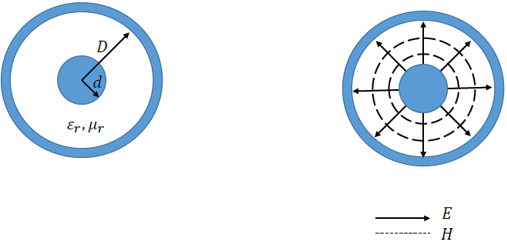
\includegraphics[width=8cm]{./images/Coax.png}
\end{minipage}
\\
\\
\\
\begin{minipage}{6cm}
	\textbf{Striplines (TEM Mode only):}\\ 
	Striplines can support TEM mode only, provided that $b<< \lambda/4$ where $\lambda$ is the wavelength in the medium.\\ \\
	$ Z_0 = \frac{30\pi}{\sqrt{\epsilon_r}}\cdot \frac{b}{W_e + 0.441\cdot b}$\\ \\
\end{minipage}
\hspace{4cm}
\begin{minipage}{8cm}
	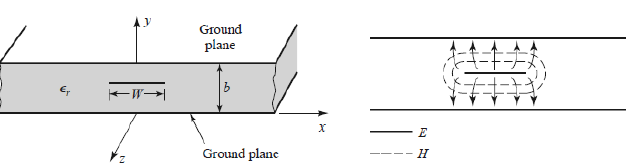
\includegraphics[width=8cm]{./images/Stripline.png}
\end{minipage}
\\
\\
\\
\\
\begin{minipage}{6cm}
	\textbf{Micro Striplines (TEM Mode only):}\\ 
	To keep the equations (field distribution) simpler  $y > d$\\
	\\
	$Z_0 =\begin{cases}&\text{$\frac{60}{\sqrt{\epsilon_e}}\ln (\frac{8d}{W}+\frac{W}{4d})$ $\hspace{3cm}$ for $ W/d \leq 1 $}\\&\text{$\frac{120\pi}{\sqrt{\epsilon_e}\cdot [W/d + 1.393 + 0.667 \ln(W/d+1.44)]} \hspace{1cm}$ for $ W/d \geq 1 $ }\end{cases}$ \\
	\\
	where $\epsilon_e$ is:\\
	\\
	$\epsilon_e \approx \frac{\epsilon_r+1}{2}+\frac{\epsilon_r-1}{2}\cdot \frac{1}{\sqrt{1+10\frac{d}{W}}}$
	
	
\end{minipage}
\hspace{4cm}
\begin{minipage}{8cm}
	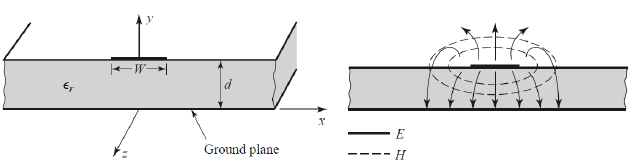
\includegraphics[width=8cm]{./images/MicroStripline.png}
\end{minipage}

\newpage
\section{Idiotenseite}
\subsection{Dreiecksformeln}
\begin{tabular}{lll}
	& \parbox{9.5cm}{
		\textbf{Cosinussatz} \\
		$$c^2 = a^2 + b^2 - 2 \cdot a \cdot b \cdot \cos \gamma$$\\
		\textbf{Sinussatz} \\
		$$\frac{a}{\sin \alpha} = \frac{b}{\sin \beta} = \frac{c}{\sin \gamma} = 2r =
		\frac{u}{\pi}$$
		\textbf{Pythagoras beim Sinus}\\
		$$\sin^2(b)+\cos^2(b)=1 \qquad \tan(b)=\frac{\sin(b)}{\cos(b)}$$}
		
	& \parbox{8cm}{
		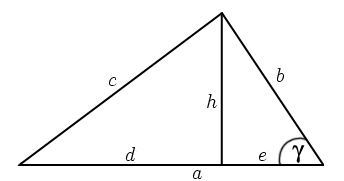
\includegraphics[width=6cm]{./idiotenseite/images/cosinussatz.png}}
\end{tabular}
\begin{center}
	\begin{multicols}{2}
		$\sin \beta = \frac ba =\frac{\text{Gegenkathete}}{\text{Hypotenuse}}$\\
		$\cos \beta = \frac ca =\frac{\text{Ankathete}}{\text{Hypotenuse}}$\\
		$\tan \beta = \frac cb =\frac{\text{Gegenkathete}}{\text{Ankathete}}$\\
		$\cot \beta = \frac cb =\frac{\text{Ankathete}}{\text{Gegenkathete}}$\\
	\end{multicols}
\end{center}

	
\subsection{Funktionswerte für Winkelargumente}
	\begin{multicols}{4}	
	\begin{tabular}[c]{|p{0.5cm}|p{0.4cm}||p{0.5cm}|p{0.5cm}|p{0.5cm}|}
	    	\hline
			deg & rad & sin & cos & tan\\
			\hline
			0\symbol{23} & 0 & 0 & 1 & 0\\
			\hline
			30\symbol{23} & $\frac{\pi}{6}$ & $\frac{1}{2}$ & $\frac{\sqrt{3}}{2}$ &
			$\frac{\sqrt{3}}{3}$\\
			\hline
			45\symbol{23} & $\frac{\pi}{4}$ & $\frac{\sqrt{2}}{2}$ & $\frac{\sqrt{2}}{2}$
			& 1\\
			\hline
			60\symbol{23} & $\frac{\pi}{3}$ & $\frac{\sqrt{3}}{2}$ & $\frac{1}{2}$ &
			$\sqrt{3}$\\
			\hline			
	\end{tabular} \\
	
	\begin{tabular}[c]{|p{0.7cm}|p{0.7cm}||p{0.7cm}|p{0.7cm}|}
	    	\hline
			deg & rad & sin & cos\\
			\hline
			90\symbol{23} & $\frac{\pi}{2}$ & 1 & 0\\
			\hline	
			120\symbol{23} & $\frac{2\pi}{3}$ & $\frac{\sqrt{3}}{2}$ & $-\frac{1}{2}$ \\
			\hline
			135\symbol{23} & $\frac{3\pi}{4}$ & $\frac{\sqrt{2}}{2}$ & $-\frac{\sqrt{2}}{2}$\\
			\hline
			150\symbol{23} & $\frac{5\pi}{6}$ & $\frac{1}{2}$ & $-\frac{\sqrt{3}}{2}$\\
			\hline
	\end{tabular} \\
	
	\begin{tabular}[c]{|p{0.7cm}|p{0.7cm}||p{0.7cm}|p{0.7cm}|}
	  	\hline
		deg & rad & sin & cos\\
		\hline
		180\symbol{23} & $\pi$ & 0 & -1\\
		\hline	
		210\symbol{23} & $\frac{7\pi}{6}$ & $-\frac{1}{2}$ & $-\frac{\sqrt{3}}{2}$\\
		\hline
		225\symbol{23} & $\frac{5\pi}{4}$ & $-\frac{\sqrt{2}}{2}$ & $-\frac{\sqrt{2}}{2}$\\
		\hline
		240\symbol{23} & $\frac{4\pi}{3}$ & $-\frac{\sqrt{3}}{2}$ & $-\frac{1}{2}$\\
		\hline
	\end{tabular} \\
	
	\begin{tabular}[c]{|p{0.7cm}|p{0.7cm}||p{0.7cm}|p{0.7cm}|}
    	\hline
		deg & rad & sin & cos\\
		\hline
		270\symbol{23} & $\frac{3\pi}{2}$ & -1 & 0\\
		\hline	
		300\symbol{23} & $\frac{5\pi}{3}$ & $-\frac{\sqrt{3}}{2}$ & $\frac{1}{2}$\\
		\hline
		315\symbol{23} & $\frac{7\pi}{4}$ & $-\frac{\sqrt{2}}{2}$ & $\frac{\sqrt{2}}{2}$\\
		\hline
		330\symbol{23} & $\frac{11\pi}{6}$ & $-\frac{1}{2}$ & $\frac{\sqrt{3}}{2}$\\
		\hline
	\end{tabular}					
\end{multicols}

\begin{minipage}{13cm}
	\subsection{Periodizität}
	$\cos(a+k\cdot2\pi)=\cos(a) \qquad \sin(a+k\cdot2\pi)=\sin(a) \qquad
	(k \in \mathbb{Z})$
	\subsection{Quadrantenbeziehungen}
	\begin{tabbing}
    	xxxxxxxxxxxxxxxxxxxxxxxxxxxxxxxxxx \= \kill
	  	$\sin(-a)=-\sin(a)$ \> $\cos(-a)=\cos(a)$\\
		$\sin(\pi - a)=\sin(a)$ \> $\cos(\pi - a)=-\cos(a)$\\
		$\sin(\pi + a)=-\sin(a)$ \> $\cos(\pi +a)=-\cos(a)$\\
		$\sin\left(\frac{\pi}{2}-a \right)=\sin\left(\frac{\pi}{2}+a \right)=\cos(a)$ \>
		$\cos\left(\frac{\pi}{2}-a \right)=-\cos\left(\frac{\pi}{2}+a \right)=\sin(a)$  
    \end{tabbing}
\end{minipage}
\begin{minipage}{5cm}
	

\subsection{Ableitungen}

\begin{tikzpicture}
	[	inner sep = 2mm,
		sin/.style={rectangle,minimum width=1.2cm,minimum height=1cm,rounded corners=5pt,draw=black,top color=green!20!black!50},
		abl/.style={rectangle}
	]
	\node at (1.2,0) (sin1) [sin] {$\sin$};
	\node at (0,-1.2) (cos2) [sin] {$-\cos$};
	\node at (1.2,-2.4) (sin2) [sin] {$-\sin$};
	\node at (2.4,-1.2) (cos1) [sin] {$\cos$};
	
	\draw[thick,black,->] (sin1.east) .. controls +(right:0.6cm) and +(up:0.6cm) ..  (cos1.north)
	node [pos=0.5,above](abl) {$\frac{d}{dx}$};
	\draw[thick,black,->] (cos1.south) .. controls +(down:0.6cm) and +(right:0.6cm) .. (sin2.east)
	node [pos=0.5,below](abl) {$\frac{d}{dx}$};
	\draw[thick,black,->] (sin2.west) .. controls +(left:0.6cm) and +(down:0.6cm) .. (cos2.south)
	node [pos=0.5,below](abl) {$\frac{d}{dx}$};
	\draw[thick,black,->] (cos2.north) .. controls +(up:0.6cm) and +(left:0.6cm) .. (sin1.west)
	node [pos=0.5,above](abl) {$\frac{d}{dx}$};
\end{tikzpicture}
\end{minipage}
\begin{multicols}{2}
	\subsection{Additionstheoreme}
	$\sin(a \pm b)=\sin(a) \cdot \cos(b) \pm \cos(a) \cdot \sin(b)$\\
	$\cos(a \pm b)=\cos(a) \cdot \cos(b) \mp \sin(a) \cdot \sin(b)$\\	
	$\tan(a \pm b)=\dfrac{\tan(a) \pm \tan(b)}{1 \mp \tan(a) \cdot \tan(b)}$
	\columnbreak
	
	\subsection{Doppel- und Halbwinkel}	
	$\sin(2a)=2\sin(a)\cos(a)$\\
	$\cos(2a)=\cos^2(a)-\sin^2(a)=2\cos^2(a)-1=1-2\sin^2(a)$\\
	$\cos^2 \left(\frac{a}{2}\right)=\frac{1+\cos(a)}{2} \qquad
	\sin^2 \left(\dfrac{a}{2}\right)=\frac{1-\cos(a)}{2}$
\end{multicols}
\begin{multicols}{2}
	\subsection{Produkte}
		$\sin(a)\sin(b)=\frac{1}{2}(\cos(a-b)-\cos(a+b))$\\
		$\cos(a)\cos(b)=\frac{1}{2}(\cos(a-b)+\cos(a+b))$\\
		$\sin(a)\cos(b)=\frac{1}{2}(\sin(a-b)+\sin(a+b))$\\
	\subsection{Euler-Formeln} 

	$\sin(x) = \frac{1}{2j} \left(e^{jx} - e^{-jx}\right) \qquad
	\cos(x) = \frac{1}{2} \left(e^{jx} + e^{-jx}\right)$ \\
	$e^{x+jy} = e^x \cdot e^{jy} = e^x \cdot \left(\cos(y) + j\sin(y)\right)$ \\
	$e^{j\pi} = e^{-j\pi} = -1$ \\
	\columnbreak
	
	\subsection{Summe und Differenz}
		$\sin(a)+\sin(b)=2 \cdot \sin \left(\frac{a+b}{2}\right) \cdot
		\cos\left(\frac{a-b}{2}\right)$\\
		$\sin(a)-\sin(b)=2 \cdot \sin \left(\frac{a-b}{2}\right) \cdot
		\cos\left(\frac{a+b}{2}\right)$\\
		$\cos(a)+\cos(b)=2 \cdot \cos \left(\frac{a+b}{2}\right) \cdot
		\cos\left(\frac{a-b}{2}\right)$\\
		$\cos(a)-\cos(b)=-2 \cdot \sin \left(\frac{a+b}{2}\right) \cdot
		\sin\left(\frac{a-b}{2}\right)$\\
		$\tan(a) \pm \tan(b)=\dfrac{\sin(a \pm b)}{\cos(a)\cos(b)}$\\
\end{multicols}

%\subsection{Quellenumwandlung}
\begin{tabular}{cccp{6cm}}
Lineare Stromquelle		& $\Longleftrightarrow$ & Lineare Spannungsquelle & Formeln \\
\raisebox{-.8\totalheight}{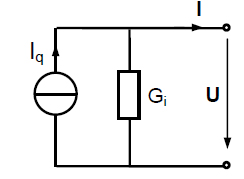
\includegraphics[width=3.5cm]{idiotenseite/images/ersatz_strom.jpg}}&
&
\raisebox{-.8\totalheight}{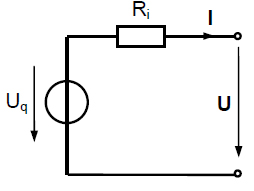
\includegraphics[width=3.5cm]{idiotenseite/images/ersatz_spannung.jpg}}
&
$I_q = \frac{U_q}{R_i} = U_q \cdot G_{i Spannungsquelle}$ \newline
$U_q = \frac{I_q}{G_i} = I_q \cdot R_{i Stromquelle}$ \newline
Der Wiederstand/Leitwert bleibt gleich \newline \\
\end{tabular}
\subsection{Superposition}
\textbf{Vorgehen:}
\begin{multicols}{2}
\begin{enumerate}
  \item Alle Quellen bis auf eine entfernen
  \item Restliche Quellen ersetzen: Stromquelle $\rightarrow$ Unterbruch,
  Spannungsquelle $\rightarrow$ Kurzschluss
  \item Teilströme mit der verbleibenden Quelle berechnen
  \item Für alle anderen Quellen das vorgehen wiederholen
  \item Alle Teilströme/-spannungen zusammenzählen
\end{enumerate}
\end{multicols}
\subsection{Einschaltvorgänge}
\subsubsection{Kondensator}
\input{idiotenseite/elektrotechnik/subsections/einschalt_kondensator}
\subsubsection{Spule}
\input{idiotenseite/elektrotechnik/subsections/einschalt_spule}


\subsection{ohmsche Leistung}
\begin{multicols}{3}
	$P=U \cdot I = I^2 \cdot R = \frac{U^2}{R}$ \\
	$P= I^2 \cdot \omega L = \frac{U^2}{\omega L}$\\
	$P= I^2 \cdot \omega C = \frac{U^2}{\omega C}$
\end{multicols}
\subsection{Strom- Spannungsquellen-Verschiebung}
\input{idiotenseite/tikz/elektrotechnik/UQuellenverschiebung1.tex}
\input{idiotenseite/tikz/elektrotechnik/UQuellenverschiebung2.tex}
\input{idiotenseite/tikz/elektrotechnik/IQuellenverschiebung1.tex}
\input{idiotenseite/tikz/elektrotechnik/IQuellenverschiebung2.tex}      
\subsection{Allgemein zeitabhängige Grössen}
	\begin{tabular}{|ll|ll|}
    \hline
	\multicolumn{2}{|l}{Arithmetischer Mittelwert, Gleichwert, Linearer MW} 
	    	& \multicolumn{2}{l|}{$X_0 = \overline{X} = X_m = \frac {1} {T} \int\limits_{t_0}^{t_0+T}
	    	x(t)dt$} \\
	\hline
	Quadratischer MW, Leistung 
		& $X^2 = \frac {1} {T} \int\limits_{t_0}^{t_0+T} x^2(t)dt$ 
		& MW $n$. Ordnung
		& $X^n = \frac {1} {T} \int\limits_{t_0}^{t_0+T} x^n(t)dt$ \\
	\hline
	Effektivwert (RMS) 
		& $X = \sqrt{X^2} = \sqrt{\frac{1}{T} \int\limits ^{t_0+T}_{t_0}{x^2(t)dt}}$
		& Gleichrichtwert 
		& $X_{|m|} = \bar{|X|} = \frac{1}{T} \int\limits_{t_0}^{t_0+T}{|x(t)| dt}$ \\
	\hline
\end{tabular}
\begin{sidewaystable}
\subsection{Eigenschaften unterschiedlicher Schwingungsformen}
\begin{center}
\begin{tabular}{|l|c|c|c|c|c|c|c|c|}
\hline
	Schwingungsform & Funktion & Gleichrichtwert & Formfaktor &
	Effektivwert & Scheitelfaktor & \textbf{$X_0$} & \textbf{$X^2$} & \textbf{var(X)} \\
\hline
	Formel &
	&
	$\overline{\left|x\right|} = \frac1T\int_{0}^{T}\left| x(t)\right|dt$&
	$\frac{X}{\overline{\left|x\right|}}$&
	$X = \sqrt{X^2} = \sqrt{\frac{1}{T} \int\limits ^{t_0+T}_{t_0}{x^2(t)dt}}$&
	$k_{s}=\frac{X_{\mathrm{max}}}{X_{\mathrm{eff}}}$&
	&
	&
	\\
\hline
	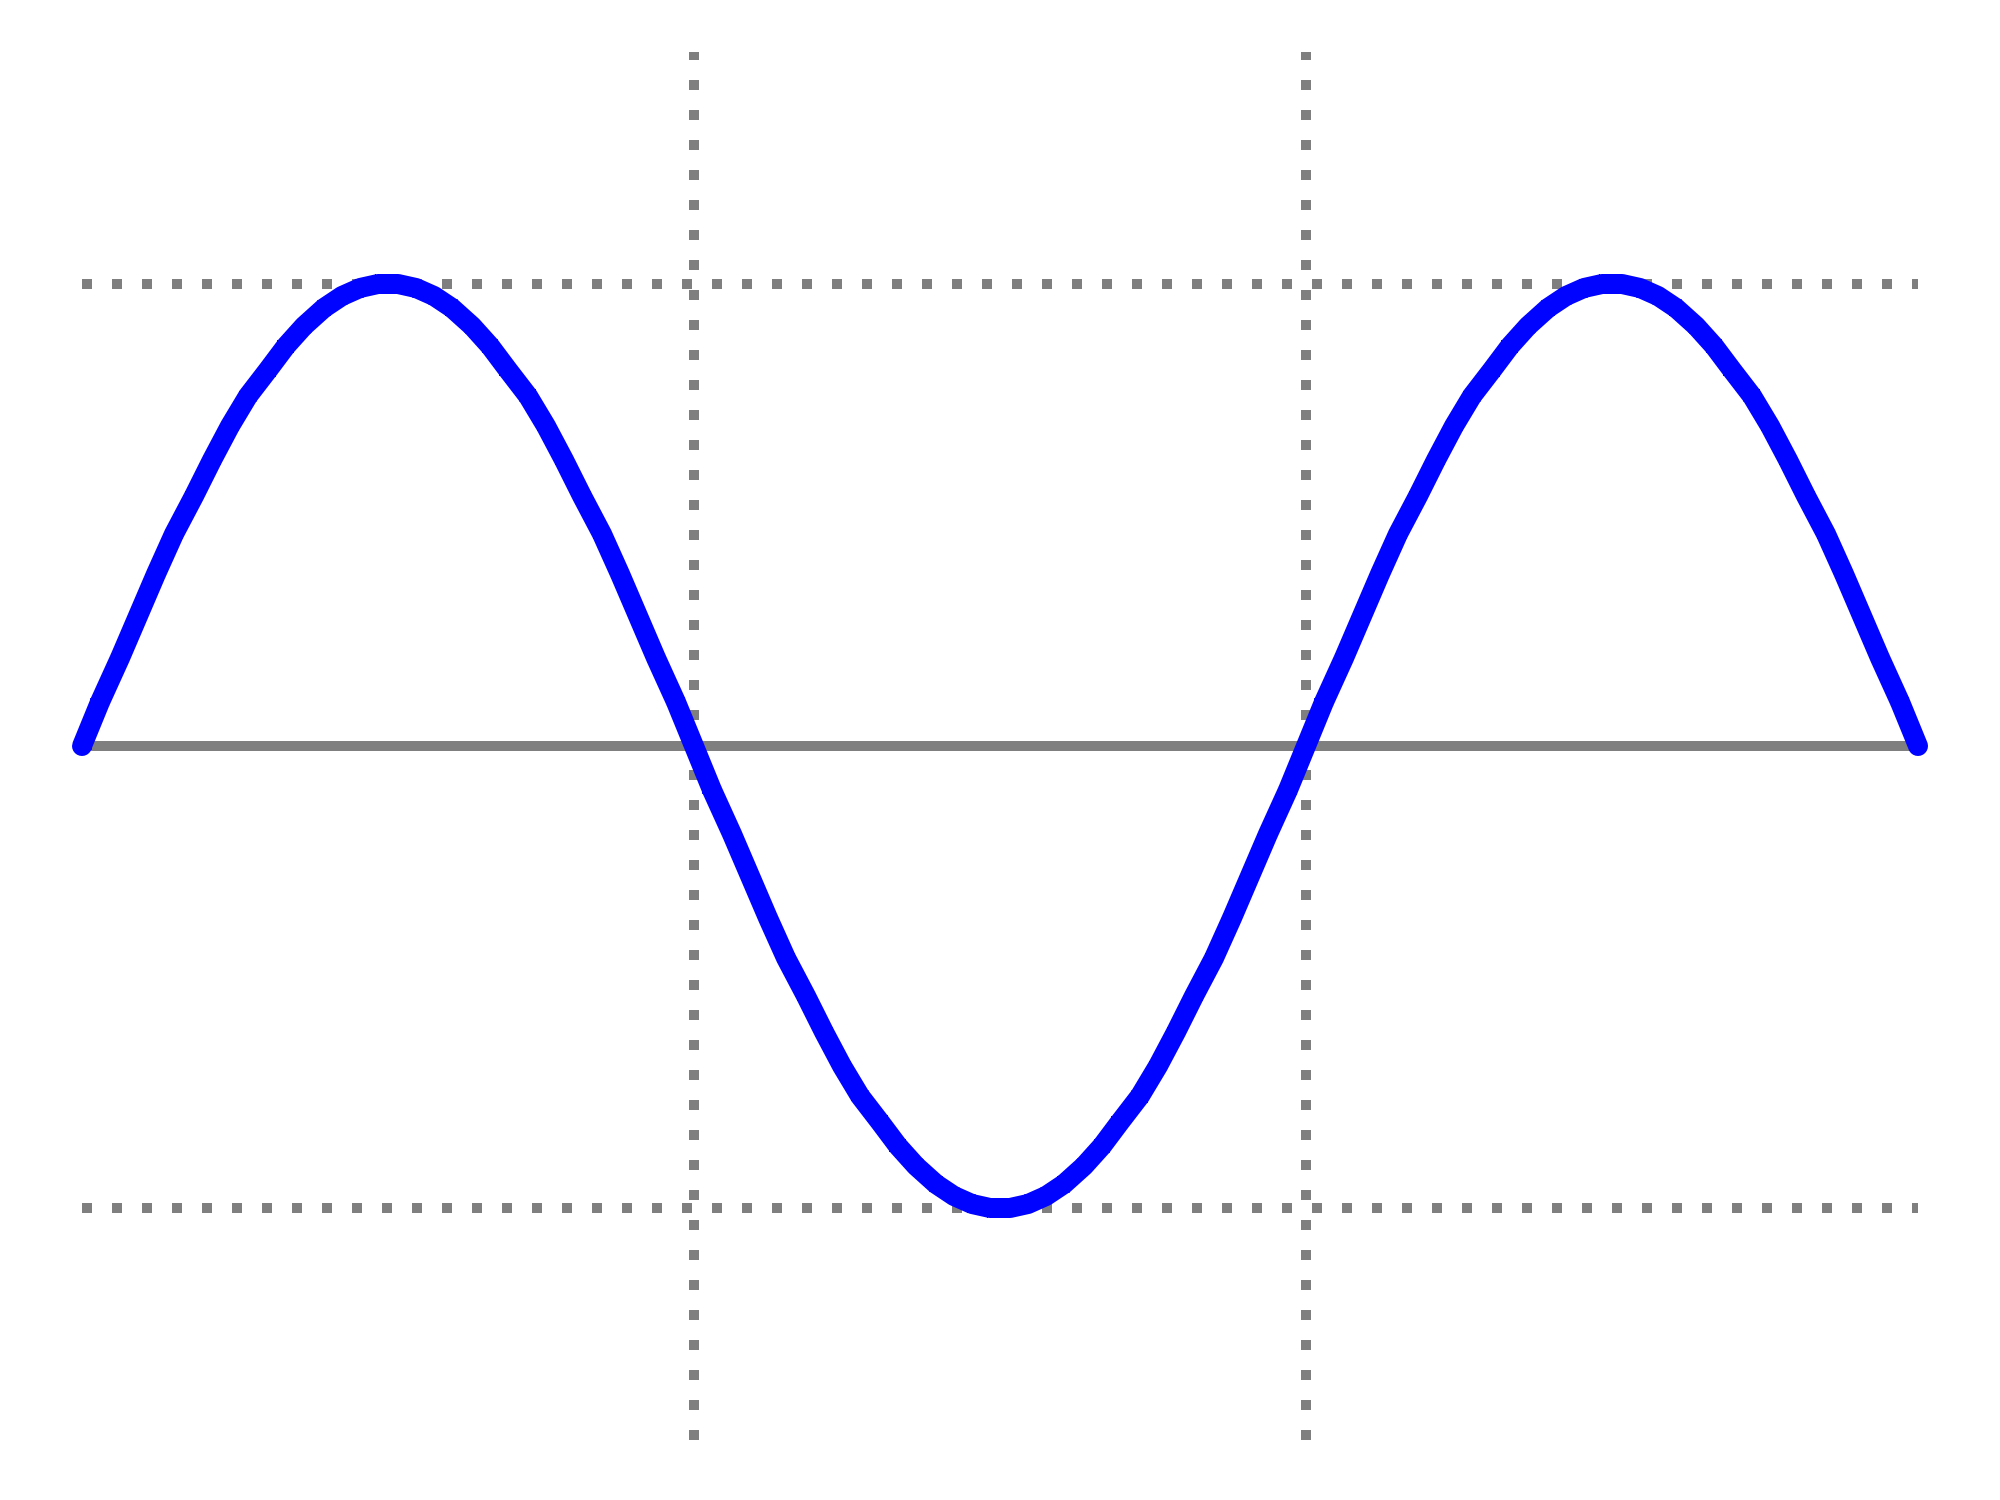
\includegraphics[width=2cm]{idiotenseite/images/table_sine_wave.png} &
	$A\cdot\sin(t)$ &
	$\frac{2}{\pi} \approx 0.637$ &
	$\frac{\pi}{2\sqrt{2}} \approx 1.11$ &
	$\frac{1}{\sqrt{2}}\approx 0.707$ &
	$\sqrt{2}\approx 1.414$ &
	$0$ &
	$\frac{A^2}{2}$ &
	$\frac{A^2}{2}$ \\
\hline	
	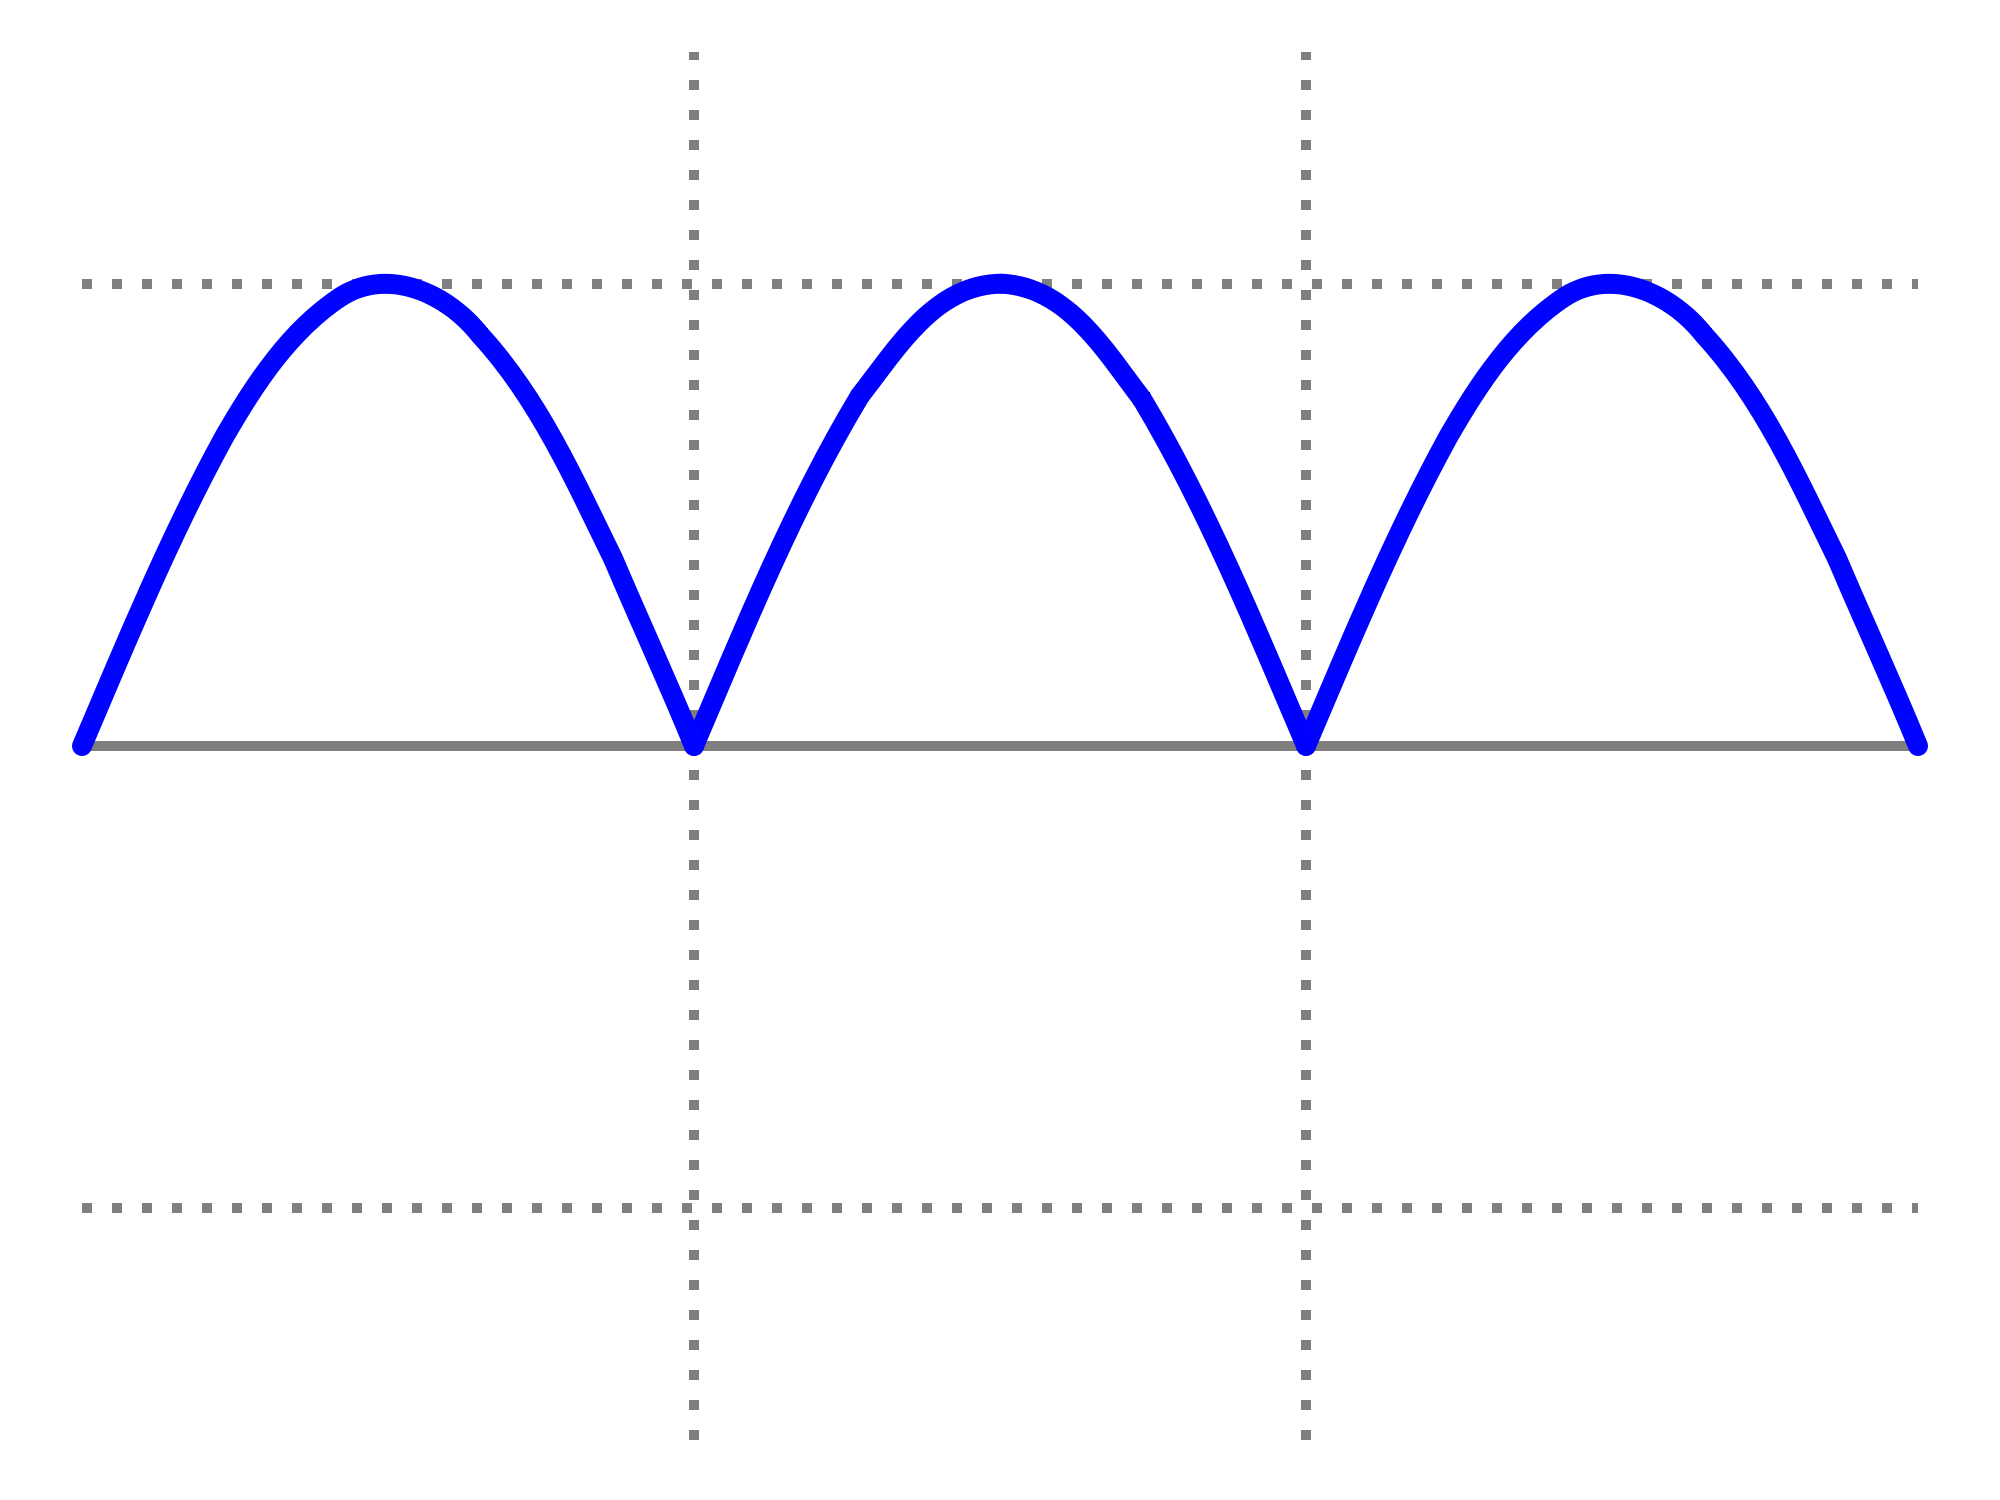
\includegraphics[width=2cm]{idiotenseite/images/table_full-wave_rectified_sine.png} &
	$A\cdot|\sin(t)|$ &
	$\frac{2}{\pi} \approx 0.637$ &
	$\frac{\pi}{2\sqrt{2}} \approx 1.11$ &
	$\frac{1}{\sqrt{2}} \approx 0.707$ &
	$\sqrt{2} \approx 1.414$  &
	$\frac{2A}{\pi}$ & $\frac{A^2}{2}$ & $\frac{A^2}{2}-\frac{4A^2}{\pi^2}$
	\\
\hline
	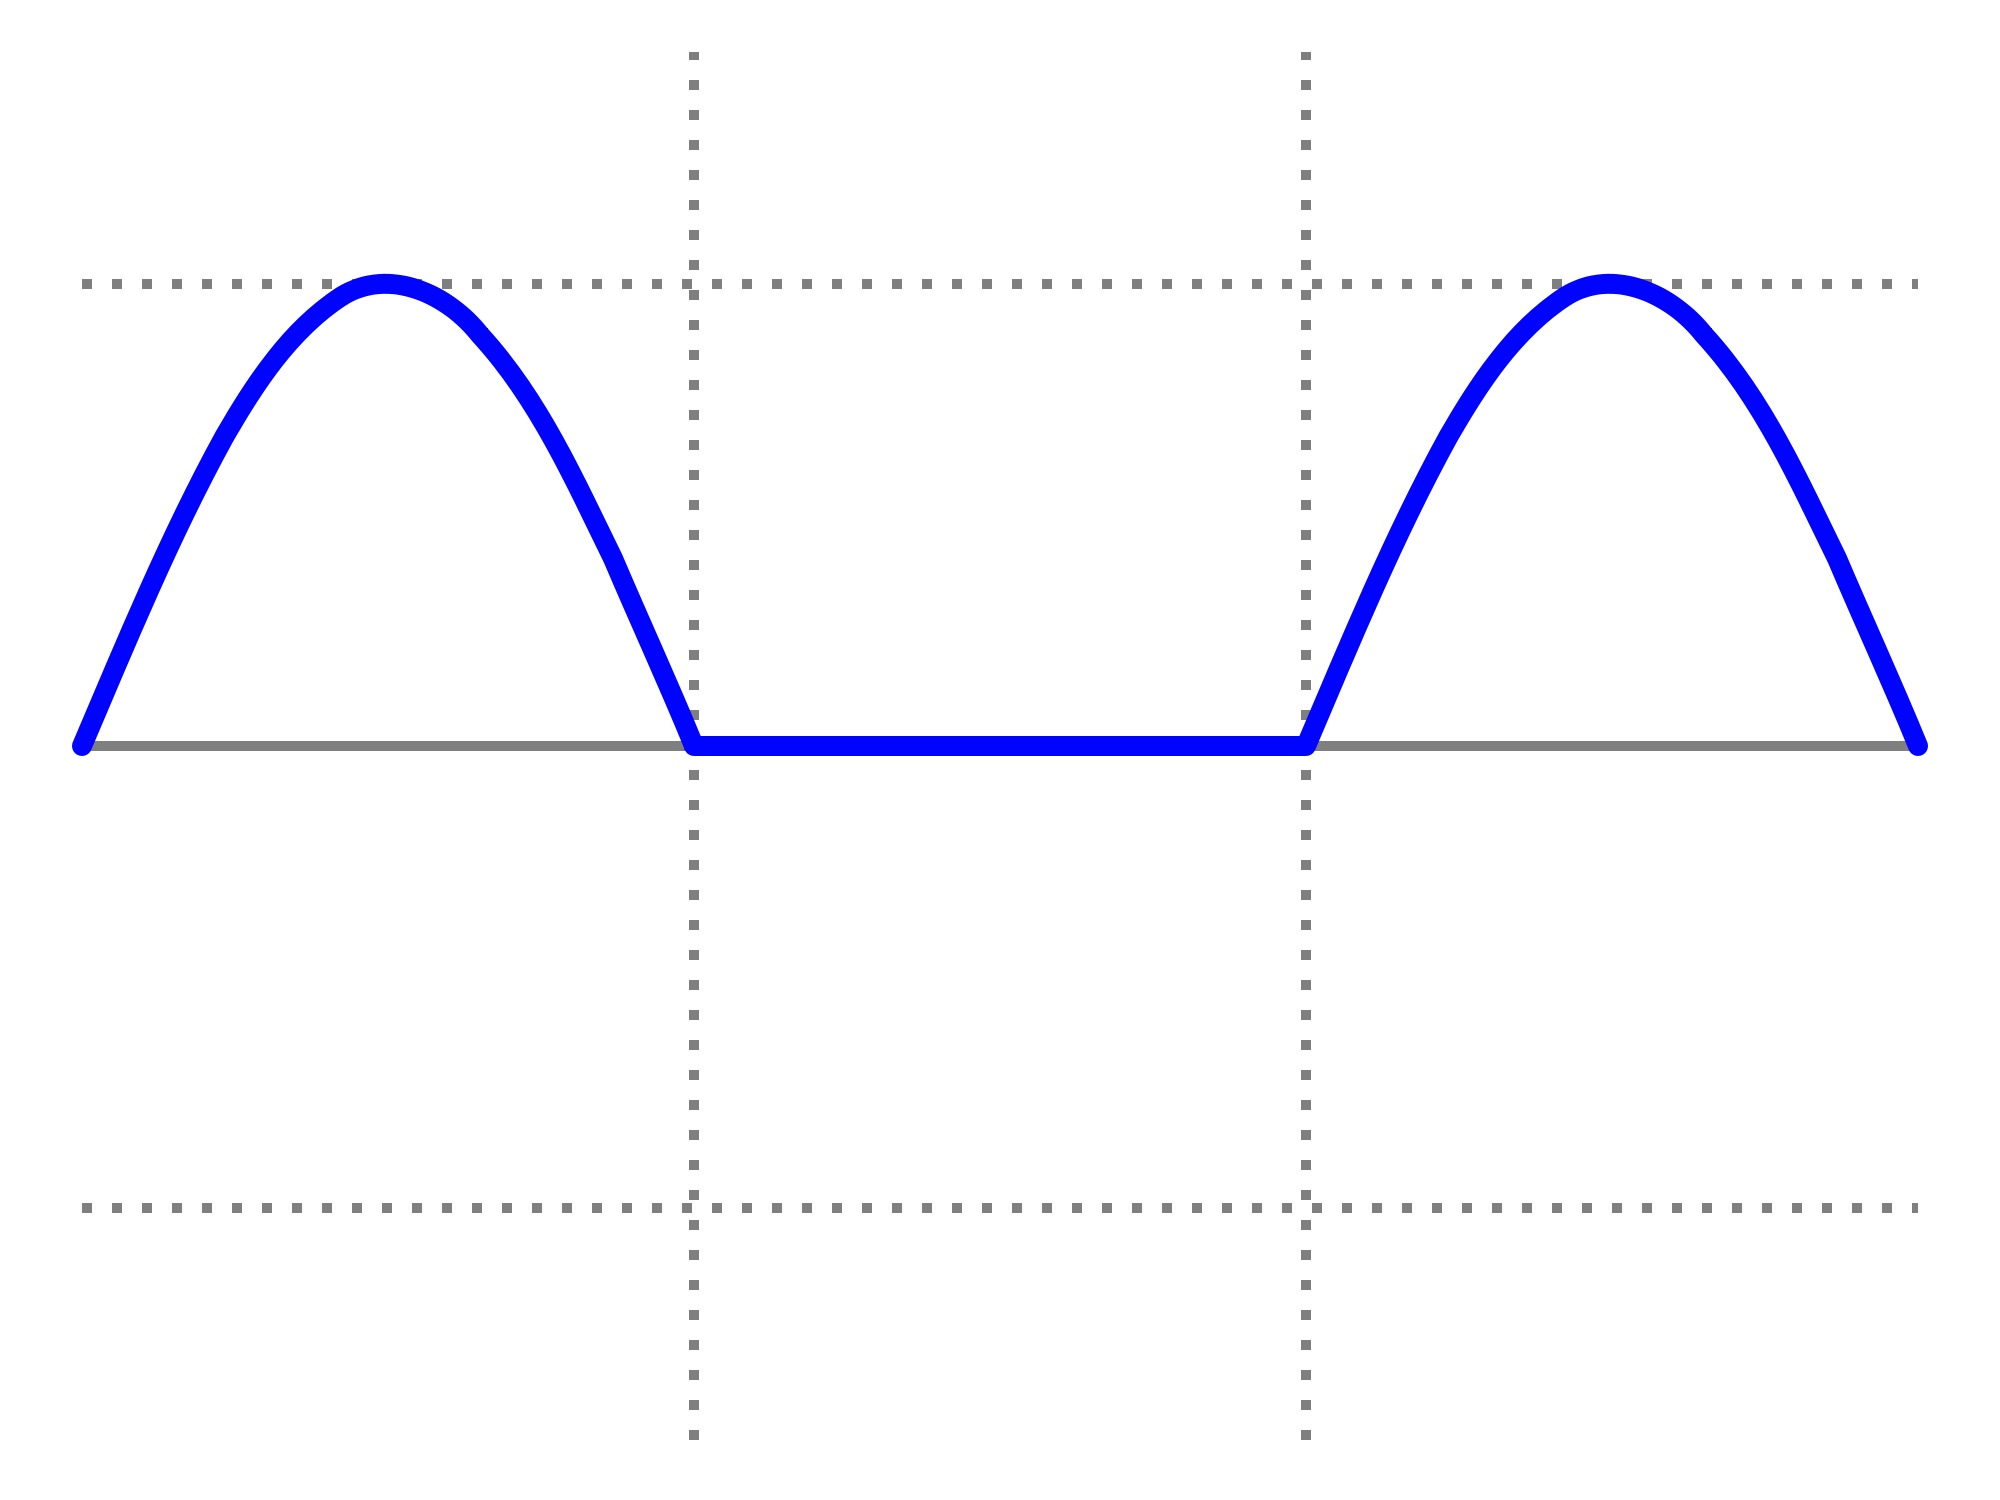
\includegraphics[width=2cm]{idiotenseite/images/table_half-wave_rectified_sine.png} &
	$\begin{cases} A\cdot\sin (t) & 0<t<\pi  \\ 0 & \text{True}\end{cases}$ &
	$\frac{1}{\pi}\approx 0.318$ &
	$\frac{\pi}{2}\approx 1.571$ &
	$\frac{1}{2} = 0.5$	&
	2  &
	$\frac{A}{\pi}$ &
	$\frac{A^2}{4}$ & $\frac{A^2}{4}-\frac{A^2}{\pi^2}$
	\\
\hline
	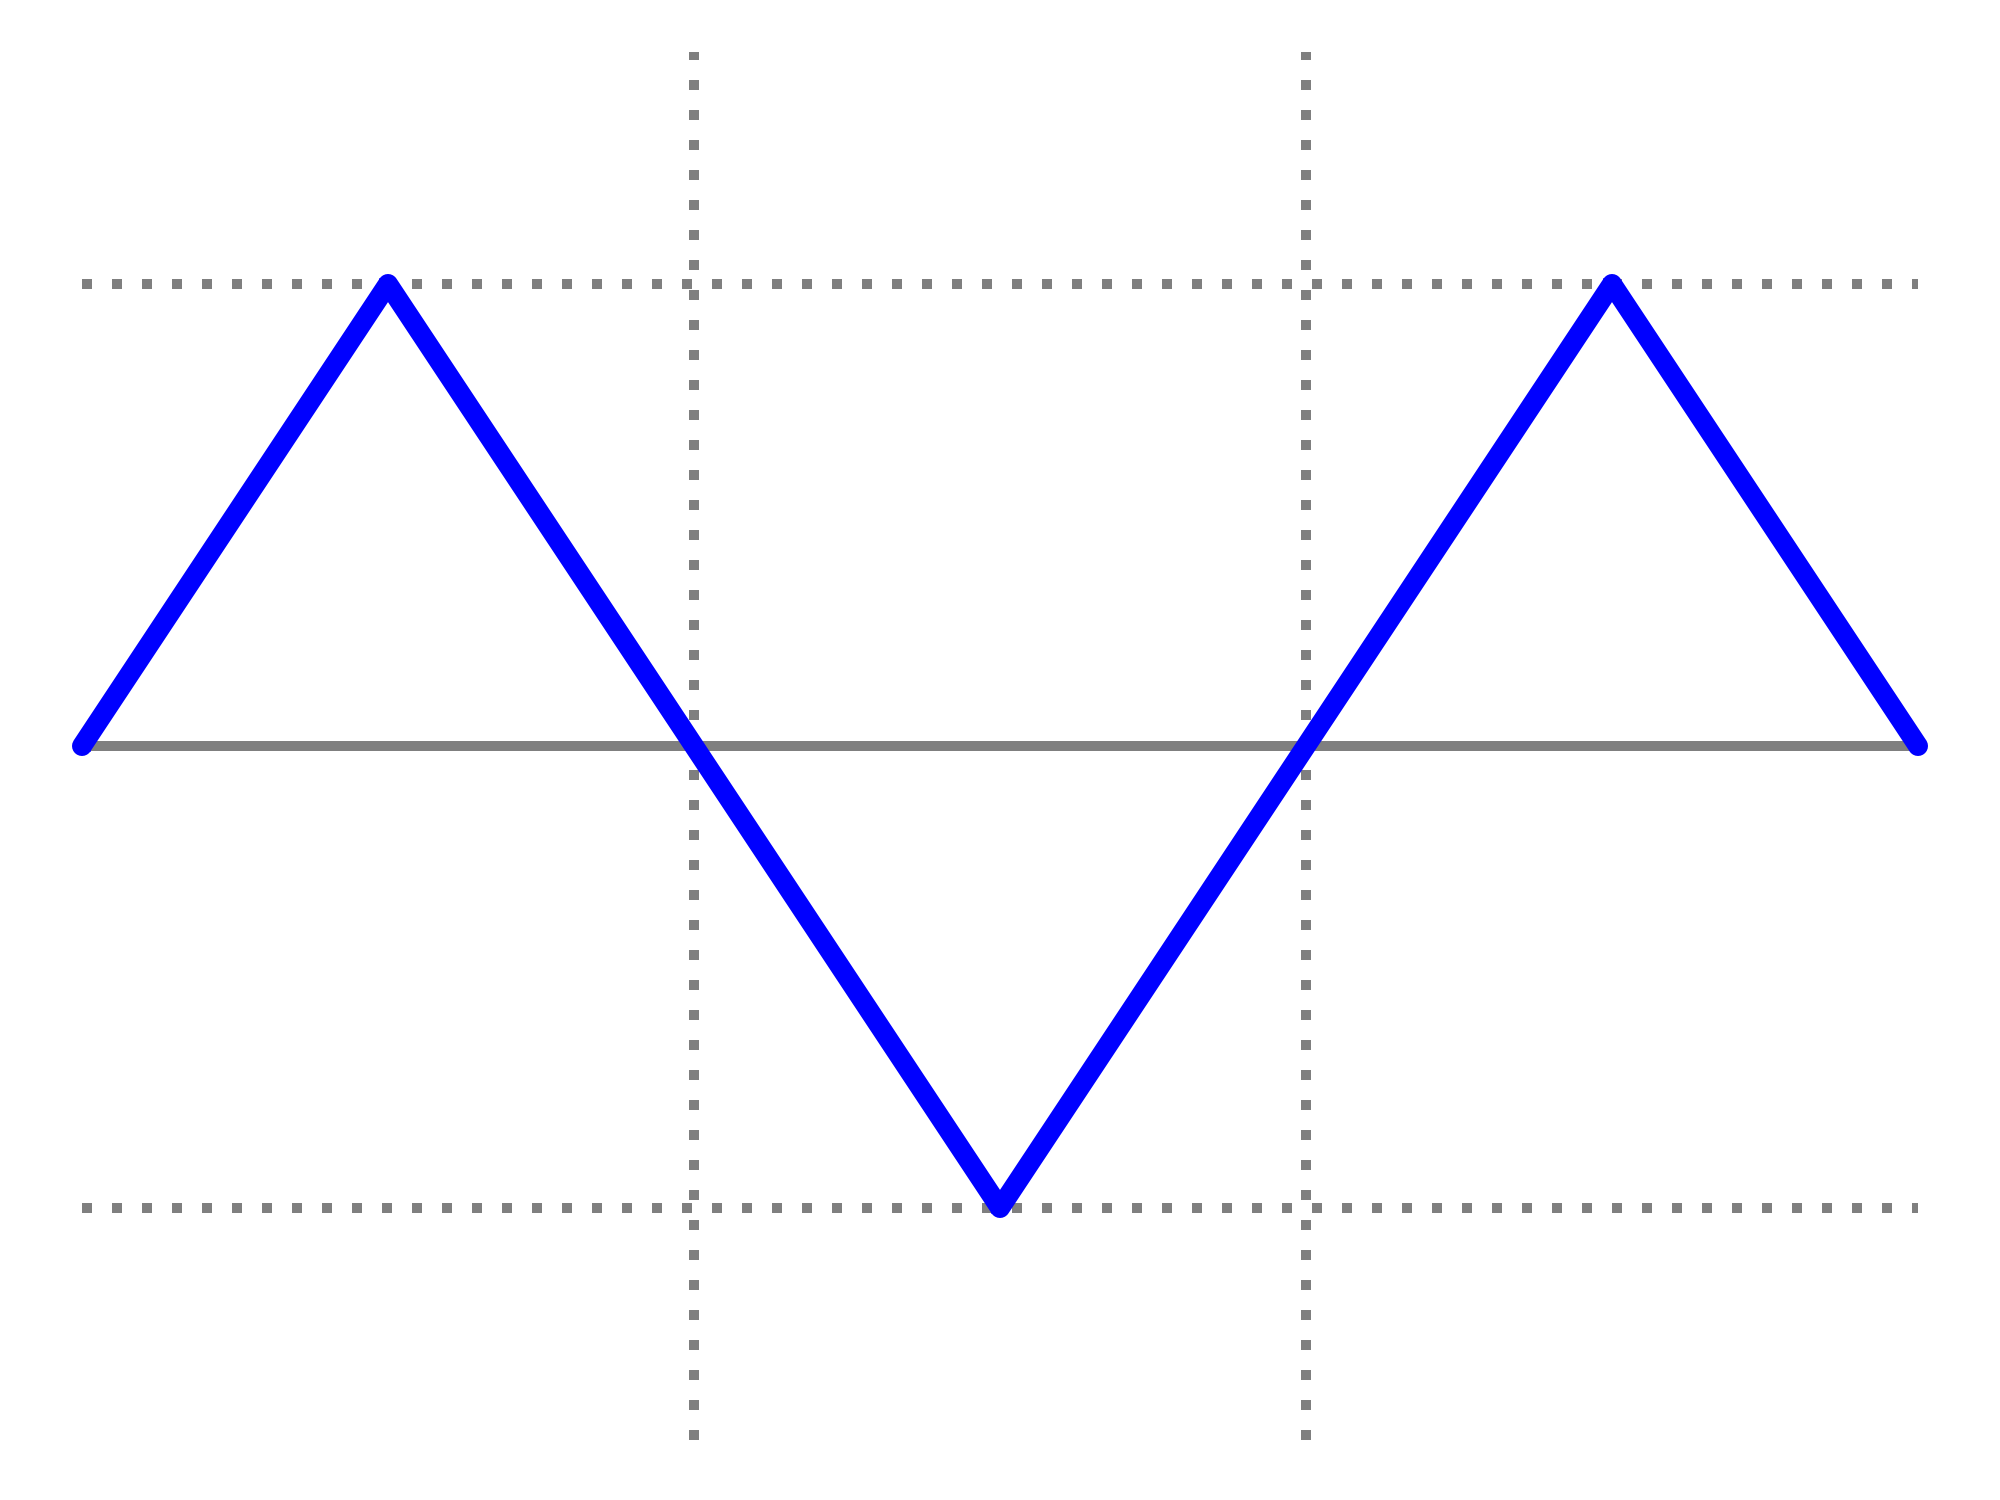
\includegraphics[width=2cm]{idiotenseite/images/table_triangle_wave.png} &
	$A\cdot\Lambda(t)$ &
	$\frac{1}{2}= 0.5$ &
	$\frac{2}{\sqrt{3}}\approx 1.155$ &
	$\frac{1}{\sqrt{3}}
	\approx 0.557$ &
	$\sqrt{3} \approx 1.732$ &
	$0$ &
	$\frac{A^2}{3}$ &
	$\frac{A^2}{3}$ \\
\hline	
	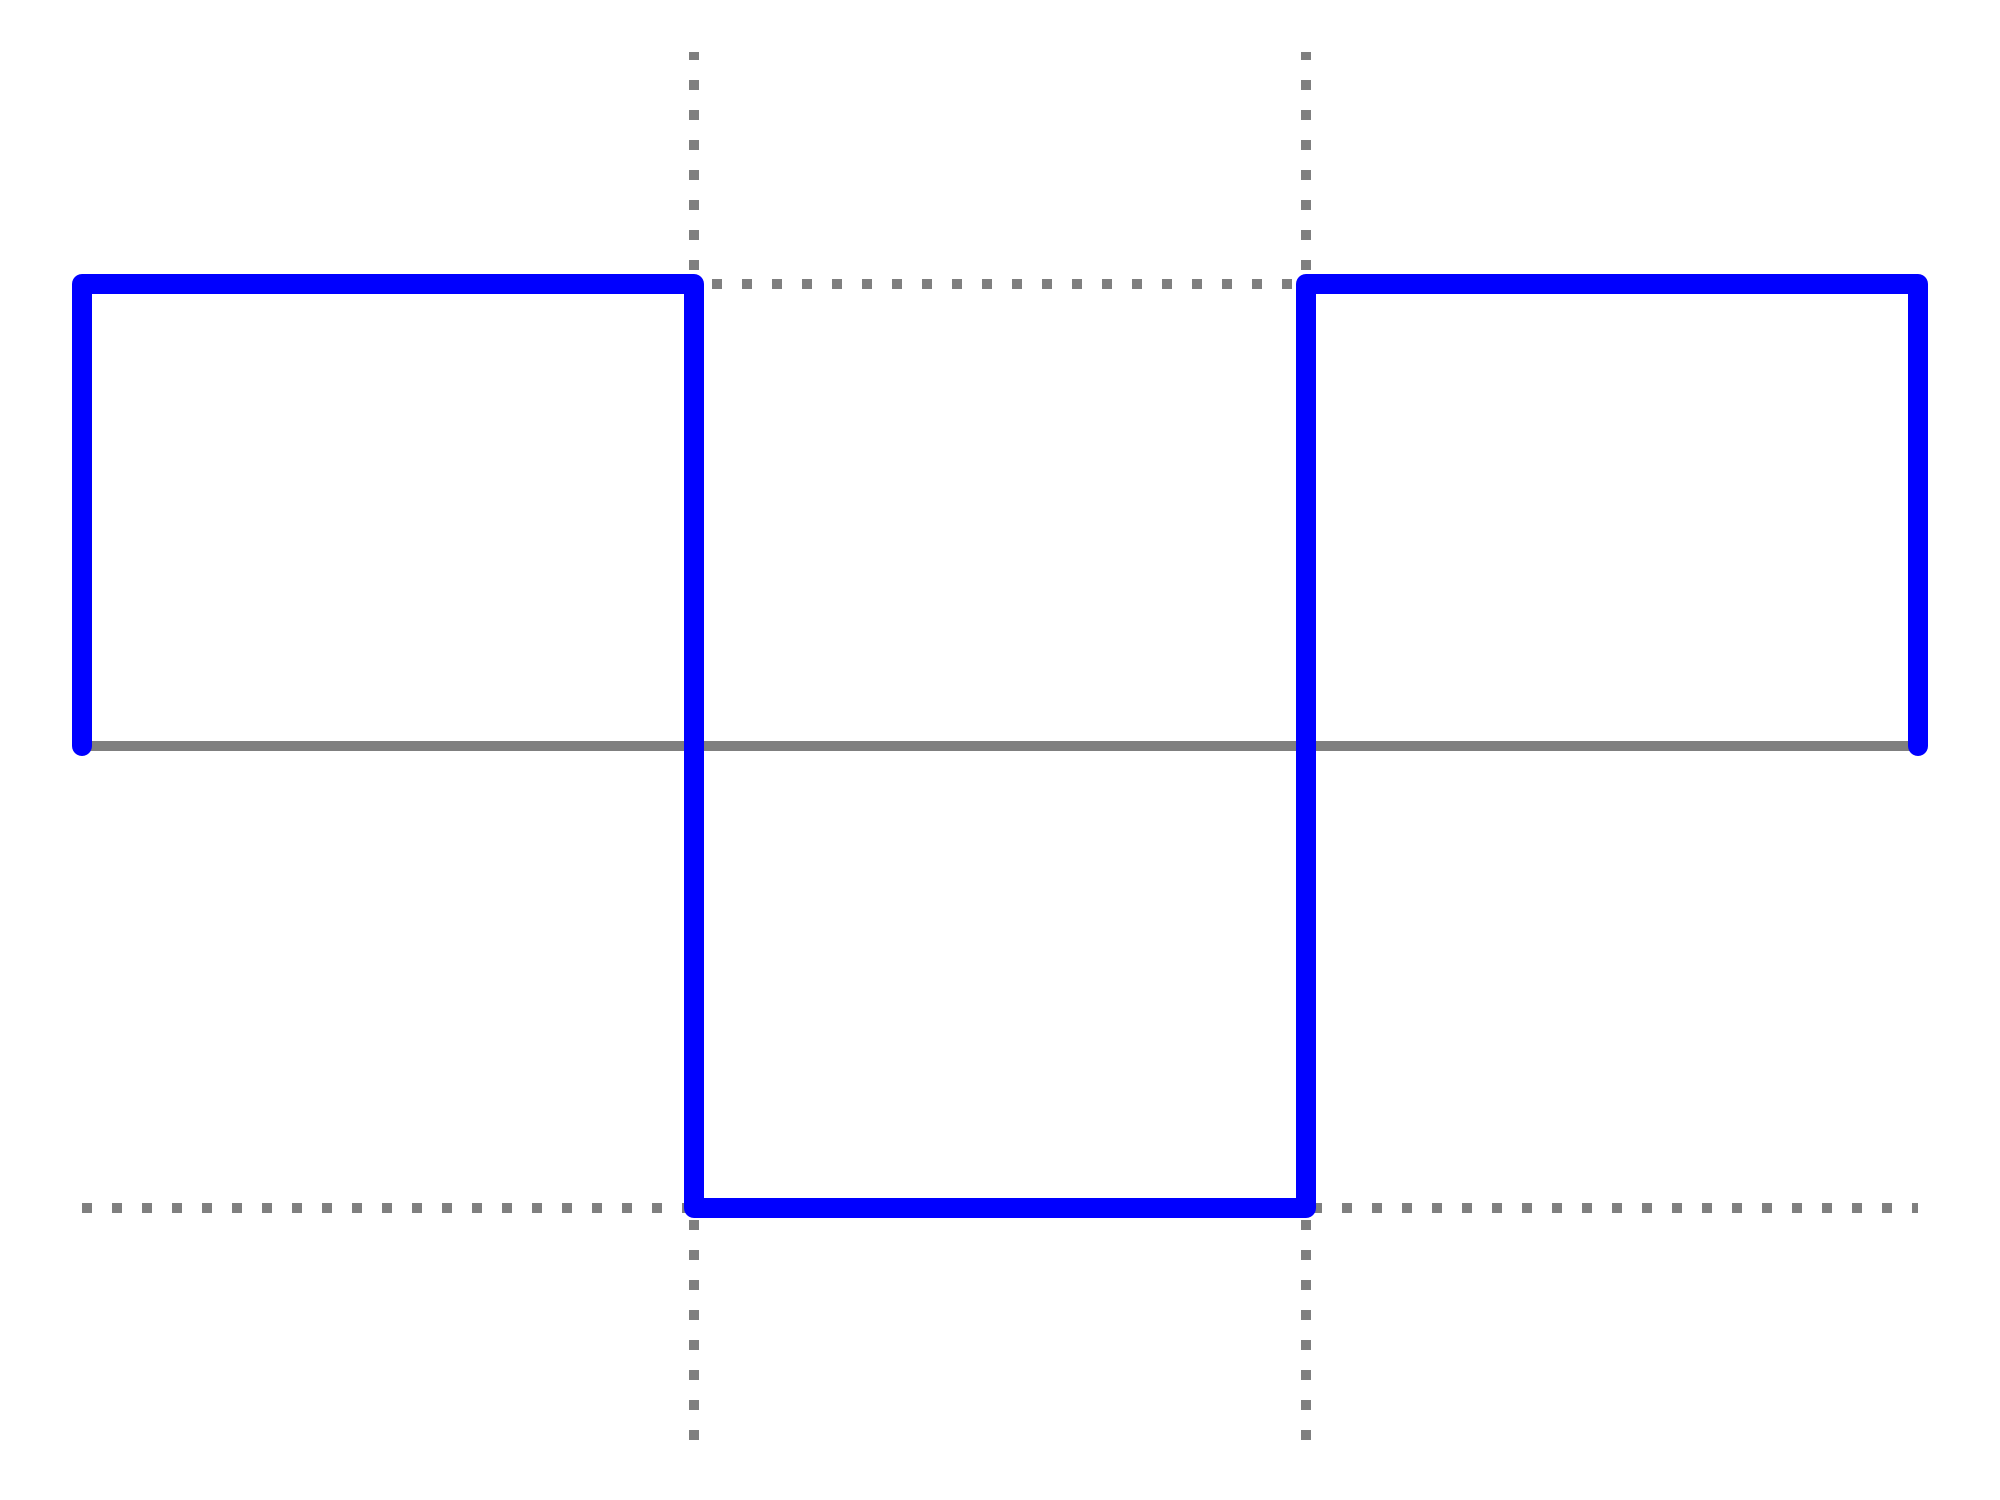
\includegraphics[width=2cm]{idiotenseite/images/table_square_wave.png} &
	$\begin{cases} A & 0<x<t \\ 0 & \text{True}\end{cases}$ &
	$1$ &
	$1$ &
	$1$ &
	$1$ &
	$0$ &
	$A^2$ &
	$A^2$ \\
\hline	
	DC&
	1&
	$1$ &
	$1$ &
	$1$ &
	$1$  &
	-&
	-&
	-\\
\hline	
	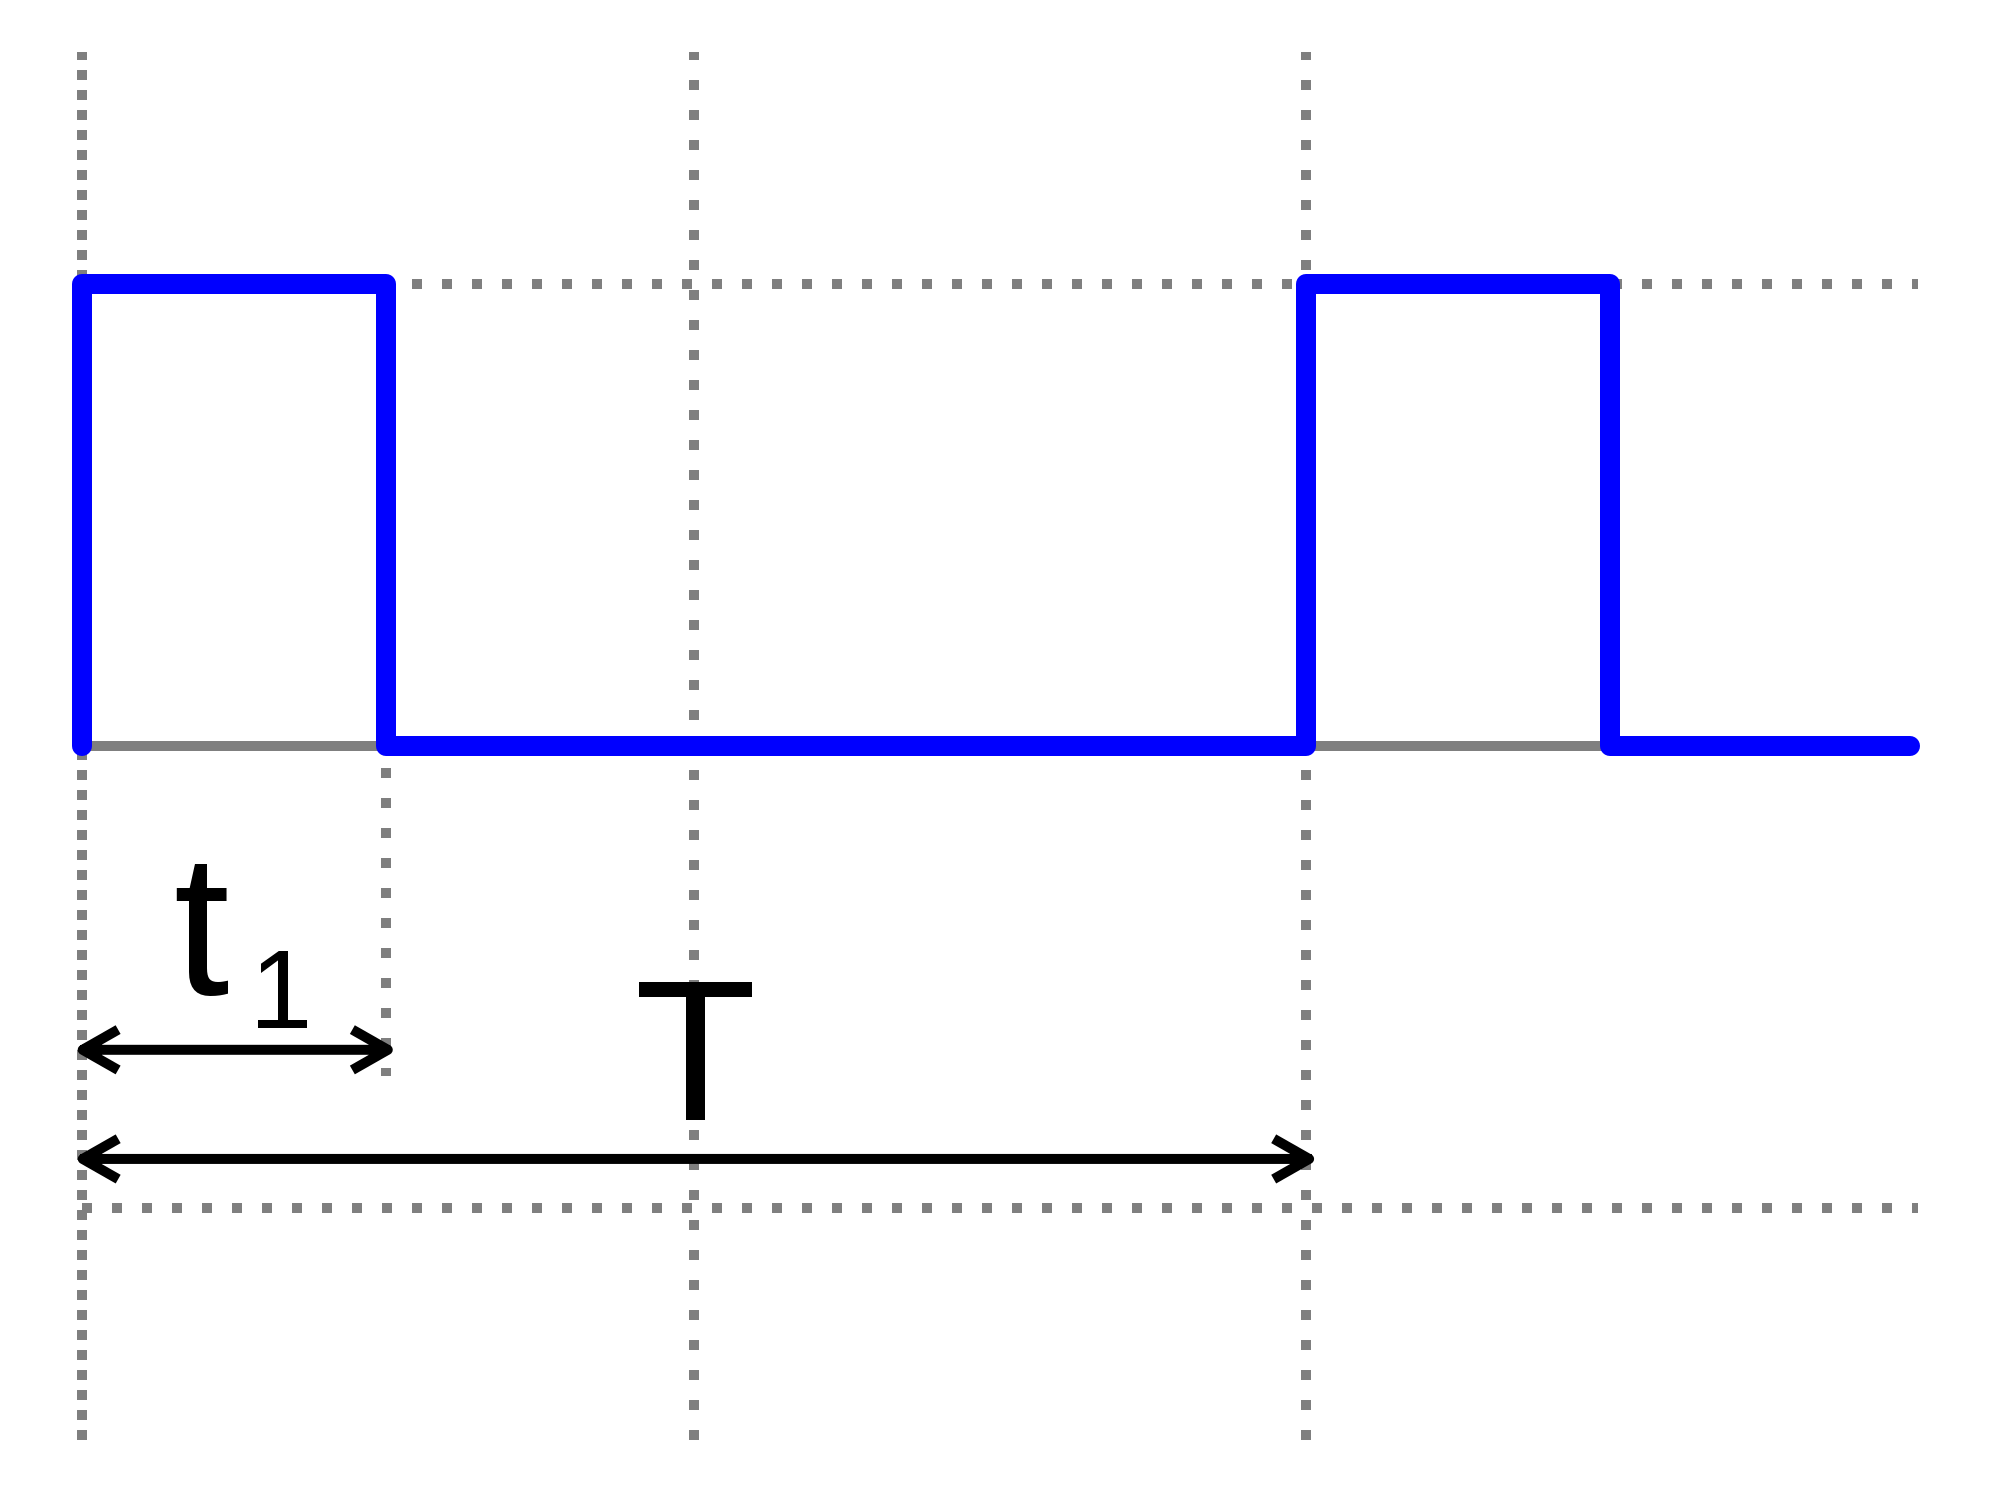
\includegraphics[width=2cm]{idiotenseite/images/table_pulse_wide_wave.png} &
	&
	$\frac{t_1}{T}$ & $\sqrt{\frac{T}{t_1}}$ & $\sqrt{\frac{t_1}{T}}$ & $\sqrt{\frac{T}{t_1}}$ &
	$A\frac{t}{T}$ &
	$A^2\frac{t}{T}$ &
	$\frac{A^2t}{T}-\frac{A^2t^2}{T^2}$\\
\hline
\end{tabular}
\end{center}
\end{sidewaystable}



\subsection{Diverses}
\begin{tabbing}
	xxxxxxxxxxxxxxxxxxxxxxxxxxxx \= xxxxxxxxxxxxxxxxxxxxxxxxxxxxxx \= \kill
 	$f'(z) = \lim \limits_{\Delta z \rightarrow 0} \frac{f(z + \Delta z) -
	f(z)}{\Delta z}$ \> $(a + b)^n = \sum_{k=0}^{n} \binom n k a^{n-k} \cdot b^k$ \>
	$(a \pm b)^3 =a^3 \pm  3 a^{2} b + 3 a b^2 \pm b^3 $\\ \\
	$x_{1,2} = \dfrac{-b \pm \sqrt{b^2 - 4ac}}{2a}$ \> $\binom n k = \dfrac{n!}{k!
	\cdot (n-k)!}$ \> $(a \pm b)^4 =a^4 \pm  4 a^{3} b + 6a^2b^2 \pm 4 a b^3 +
	b^4$\\
\end{tabbing}
\subsection{Reihenentwicklungen}
\begin{tabular}{llll}
\textbf{Geometrische Reihe}
	& $\sum\limits_{n=0}^{\infty} x^n$ 
	& $= \dfrac{1}{1-x}$
	& $|x| < 1$ \\
	
	& $\sum\limits_{k=0}^{\infty} k \, x^k$ & $= x \sum\limits_{k=1}^{\infty} k \,
	x^{k-1} = \dfrac{x}{(1-x)^2} $ 
	& $x \neq 1$ \\
    & $\sum\limits_{k=0}^{n} a_0\cdot q^k$ & $= a_0 \dfrac{1-q^{n+1}}{1-q}$
    & $q \neq 1$\\
\textbf{Binominalreihe} 
	& $\sum\limits_{n=0}^\infty \binom{\alpha}{n} x^n $ &$= (1+x)^\alpha$
	& $x \in (-1,1)$ \\
\textbf{E-Funktion}
	& $\sum\limits_{k = 0}^{\infty} \dfrac{x^k}{k!}$ &$ = e^x$
	& 
\end{tabular}

\subsection{Kurven}
\begin{multicols}{4}
\subsubsection{e-Funktion}
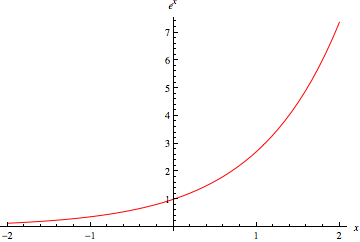
\includegraphics[width=4.5cm]{idiotenseite/images/Exp.png}
\subsubsection{Sinus-Funktion}
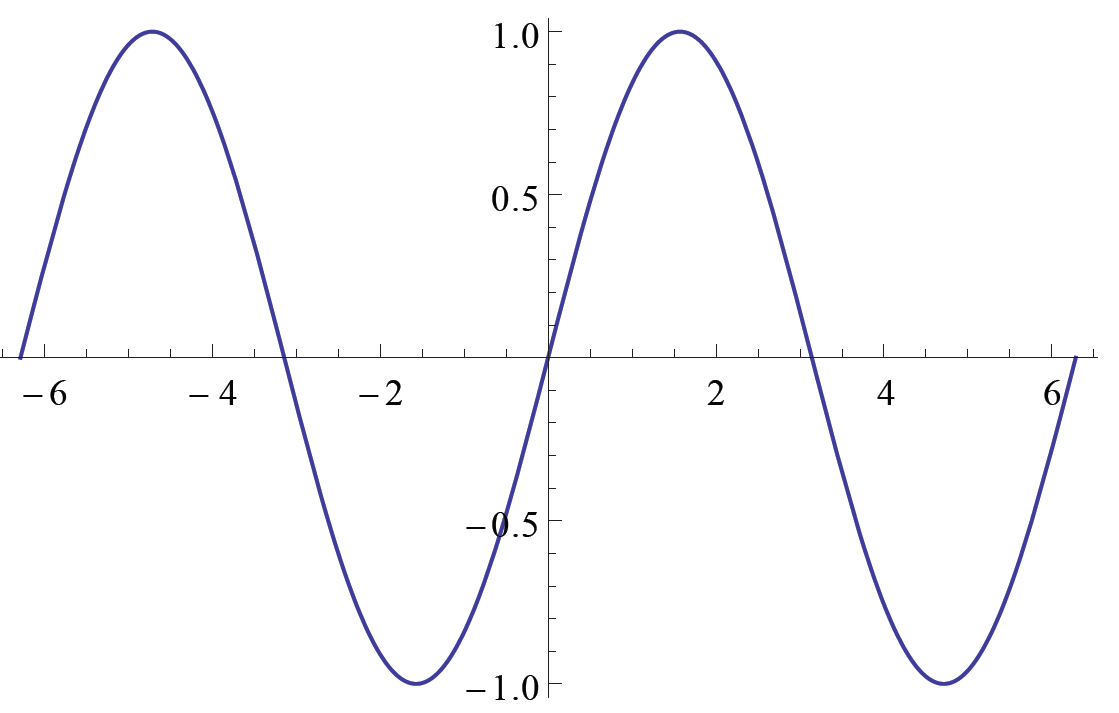
\includegraphics[width=4.5cm]{idiotenseite/images/sin.png}
\subsubsection{Cosinus-Funktion}
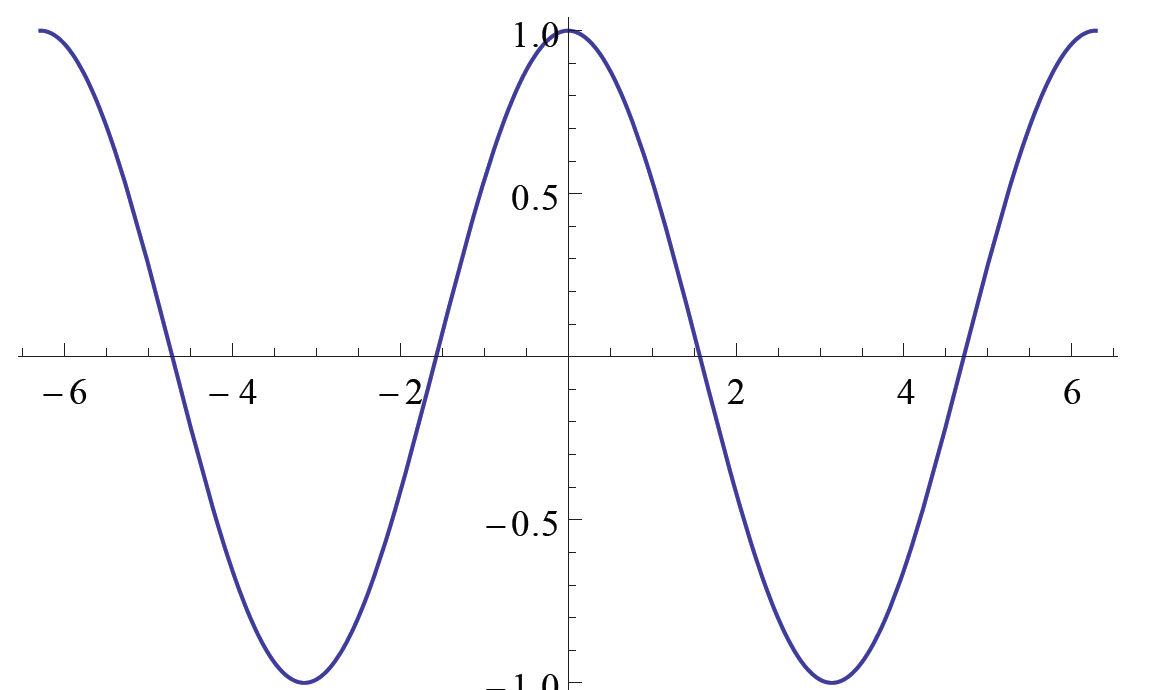
\includegraphics[width=4.5cm]{idiotenseite/images/cos.png}
\subsubsection{Tangens-Funktion}
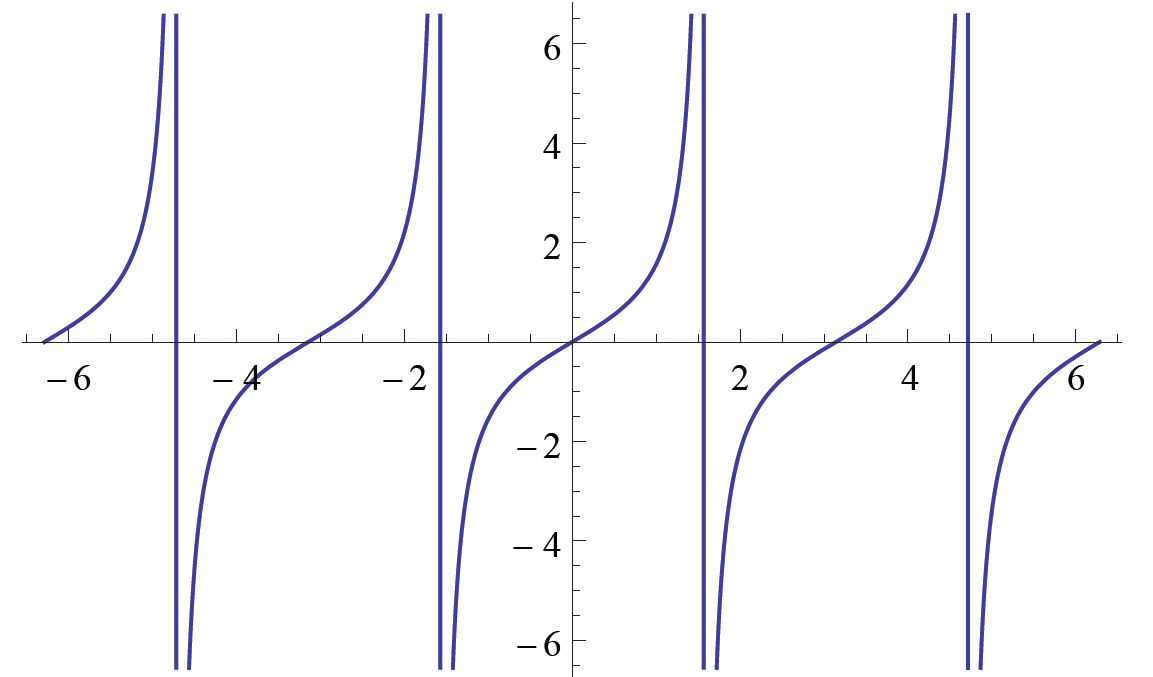
\includegraphics[width=4.5cm]{idiotenseite/images/tan.png}
\end{multicols}
%\subsection{Idiotenformel}
Wenn ihr wissen wollt was die Formel besagt dann kauft euch doch nächstes mal
die Pro Version der Formelsammlung. Arme Schmarotzer und asoziale Personen
dürfen gerne lange darüber Rätseln was das hier soll. Aber wer zu doof ist eine
Formelsammlung ehrlich zu erwerben hat sowieso keine Chance. Haha.\\
$\frac{1}{F_{Siedlungsfl\ddot ache}}\cdot\int\limits_{\vec{x} \in
Siedlungsfl\ddot ache} \frac{1}{\int\limits_{\vec{y}\in Siedlungsfl\ddot ache\ und \left|\vec{x}-\vec{y} \right|<BH}\vec{dy}} \int\limits_{\vec{y}\in Siedlungsfl\ddot ache\ und \left|\vec{x}-\vec{y} \right|<BH} \sqrt{\frac{2\cdot\left|\vec{x}-\vec{y}\right|}{1m}+1}-1\vec{dy}\vec{dx}\frac{DSE}{m^2}$

\subsection{SI-Vorsätze}

\begin{multicols}{2}
\begin{tabular}{|l|l|l|l|}
\hline
\textbf{Symbol}	& \textbf{Name} & \textbf{Wert} & \textbf{Binär} \\
\hline
da	& Deka 	& $10^1$ & \\
\hline
h	& Hekto & $10^2$ & \\ 
\hline
k	& Kilo	& $10^3$ & $2^{10} = 1024$ \\
\hline
M	& Mega	& $10^6$ & $2^{20}$\\
\hline
G	& Giga  & $10^9$ & $2^{30}$\\
\hline
T	& Tera	& $10^{12}$ & $2^{40}$ \\
\hline
P	& Peta	& $10^{15}$ & $2^{50}$\\
\hline
\end{tabular}

\columnbreak

\begin{tabular}{|l|l|l|}
\hline
\textbf{Symbol}	& \textbf{Name} & \textbf{Wert} \\
\hline
d	& Dezi	& $10^{-1}$ \\
\hline
c	& Centi	& $10^{-2}$ \\ 
\hline
m	& Milli	& $10^{-3}$ \\
\hline
y, $\mu$ & Mikro & $10^{-6}$ \\
\hline
n	& Nano	& $10^{-9}$ \\
\hline
p	& Piko	& $10^{-12}$ \\
\hline
f	& Femto & $10^{-15}$ \\
\hline
\end{tabular}
\end{multicols}
\subsection{GrichischesAlphabet}
\begin{multicols}{2}
	\subsubsection{klein}
	\begin{tabular}{ |l|l|l|l|l|l|l|l|}
		\hline
		$\alpha$&Alpha&$\theta$&Theta&o&o&$\tau$&Tau\\
		\hline
		$\beta$&Beta&$\vartheta$&Theta&$\pi$&Pi&$\upsilon$&Ypsilon\\
		\hline
		$\gamma$&Gamma&$\gamma$&Gamma&$\varpi$&Pi&$\phi$&Phi\\
		\hline
		$\delta$&Delta&$\kappa$&Kappa&$\rho$&Roh&$\varphi$&Phi\\
		\hline
		$\epsilon$&Epsilon&$\lambda$&Lambda&$\varrho$&Roh&$\chi$&Chi\\
		\hline
		$\varepsilon$&Epsilon&$\mu$&Mu&$\sigma$&Sigma&$\psi$&Psi\\
		\hline
		$\zeta$&Zeta&$\nu$&Nu&$\varsigma$&Sigma&$\omega$&Omega\\
		\hline
		$\eta$&Eta&$\xi$&Xi&&&&\\
		\hline
	\end{tabular}
	\columnbreak
	
	\subsubsection{gross}
	\begin{tabular}{|l|l|l|l|l|l|l|l|}
		\hline
		$\Gamma$&Gamma&$\Lambda$&Lambda&$\Sigma$&Sigma&$\Psi$&Psi\\
		\hline
		$\Delta$&Delta&$\Xi$&Xi&$\Upsilon$&Ypsilon&$\Omega$&Omega\\
		\hline
		$\Theta$&Theta&$\Pi$&Pi&$\Phi$&Phi&&\\
		\hline
	\end{tabular}
\end{multicols}
\begin{sidewaystable}
\subsection{Einige unbestimmte Integrale\formelbuch{1074}}
\label{unbestimmte_integrale}
\begin{tabular}{|p{12cm}|p{13cm}|}
  \hline
  
    $ \int dx=x+C $ &
     $ \int{x^\alpha}dx=\frac{x^{\alpha+1}}{\alpha+1}+C,\ x \epsilon \mathbb
    R ^+,\ \alpha \epsilon \mathbb R \backslash \{ -1 \} $ \\\hline
     $ \int{\frac{1}{x}}dx=\ln \left| x \right| + C,\ x\neq0 $ &
     $ \int{e^x}dx=e^x+C $ \\\hline
     $ \int{a^x}dx=\frac{a^x}{\ln{a}}+C,\ a \epsilon \mathbb 
    R^+\backslash\{1\} $ &
     $ \int{ \sin{x}} dx = -\cos{x} + C $ \\\hline
     $ \int{\cos{x}} dx = \sin{x} + C $ &
     $ \int{\frac{dx}{\sin^2x}}=-\cot{x}+C,\ x\neq k\pi\ \mathrm{mit}\ k
    \epsilon \mathbb Z $ \\\hline
     $ \int{\frac{dx}{\cos^2x}}=\tan{x}+C,\ x\neq\frac{\pi}{2}+k\pi\
    \mathrm{mit} k \epsilon \mathbb Z $ & 
    
    %10. :
     $ \int{\sinh{x}}dx = \cosh{x}+C $ \\ \hline
     $ \int{\cosh{x}}dx = \sinh{x}+C $ &
     $ \int{\frac{dx}{\sinh^2x}}=-\coth{x}+C,\ x\neq0 $ \\\hline
     $ \int{\frac{dx}{\cosh^2x}}=\tanh{x}+C $ &
     $ \int{\frac{dx}{ax+b}} = \frac{1}{a}\ln \left|ax + b\right| + C,\
    a\neq 0,x\neq-\frac{b}{a} $ \\\hline
     $ \int{\frac{dx}{a^2x^2+b^2}}=\frac{1}{ab}\arctan{\frac{a}{b}x}+C,\
    a\neq0,\ b\neq0 $ &
     $
    \int{\frac{dx}{a^2x^2-b^2}}=\frac{1}{2ab}\ln{\left|\frac{ax-b}{ax+b}\right|}+C,\
    a\neq0,\ b\neq0,\ x\neq\frac{b}{a},\ x\neq-\frac{b}{a} $ \\\hline
     $
    \int{\sqrt{a^2x^2+b^2}}dx=\frac{x}{2}\sqrt{a^2x^2+b^2}+\frac{b^2}{2a}\ln{(ax+\sqrt{a^2x^2+b^2})}+C,\
    a\neq0,\ b\neq0 $ &
     $
    \int{\sqrt{a^2x^2-b^2}}dx=\frac{x}{2}\sqrt{a^2x^2-b^2}-\frac{b^2}{2a}\ln\left|ax+\sqrt{a^2x^2-b^2}\right|+C,\
    a\neq0,\ b\neq0,a^2x^2\geqq b^2$ \\\hline
     $
    \int\sqrt{b^2-a^2x^2}dx=\frac{x}{2}\sqrt{b^2-a^2x^2}+\frac{b^2}{2a}\arcsin\frac{a}{b}x+C,\
    a\neq0,\ b\neq0,\ a^2x^2\leqq b^2 $ &
    %20.:
     $
    \int\frac{dx}{\sqrt{a^2x^2-b^2}}=\frac{1}{a}\ln(ax+\sqrt{a^2x^2+b^2})+C,\
    a\neq0,\ b\neq0 $ \\\hline
     $
    \int\frac{dx}{\sqrt{a^2x^2-b^2}}=\frac{1}{a}\ln\left|ax+\sqrt{a^2x^2-b^2}\right|+C,\
    a\neq0,\ b\neq0,\ a^2x^2>b^2 $ &
     $ \int\frac{dx}{\sqrt{b^2-a^2x^2}}=\frac{1}{a}\arcsin\frac{a}{b}x+C,\
    a\neq0,\ b\neq0,\ a^2x^2<b^2 $ \\\hline
     Die Integrale $\int\frac{dx}{X}, \int\sqrt{X}dx,
    \int\frac{dx}{\sqrt{X}}$ mit $X=ax^2+2bx+c,\ a\neq0 $ werden durch 
    die Umformung $X=a(x+\frac{b}{a})^2+(c-\frac{b^2}{a}) $ und die
    Substitution $ t=x+\frac{b}{a} $ in die oberen 4 Zeilen
    transformiert. & $ \int\frac{xdx}{X}=\frac{1}{2a}\ln\left|X\right|-\frac{b}{a}\int\frac{dx}{X},\
    a\neq0,\ X=ax^2+2bx+c $ \\\hline
     $ \int\sin^2axdx=\frac{x}{2}-\frac{1}{4a}\cdot\sin2ax+C,\ a\neq0 $ &
     $ \int\cos^2axdx=\frac{x}{2}+\frac{1}{4a}\cdot\sin2ax+C,\ a\neq0 $ \\\hline
     $ \int\sin^naxdx=-\frac{sin^{n-1}ax\cdot\cos
    ax}{na}+\frac{n-1}{n}\int\sin^{n-2}axdx,\ n \epsilon \mathbb N,\ a\neq0 $ &
     $ \int\cos^naxdx=\frac{\cos^{n-1}ax\cdot\sin
    ax}{na}+\frac{n-1}{n}\int\cos^{n-2}axdx,\ n\epsilon \mathbb N,\ a\neq0 $
    \\\hline
     $ \int\frac{dx}{\sin ax} =
    \frac{1}{a}\ln\left|\tan\frac{ax}{2}\right|+C,\ a\neq0,\ x\neq
    k\frac{\pi}{a}\ \mathrm{mit}\ k\epsilon\mathbb Z$ &
    %30.:
     $ \int\frac{dx}{\cos
    ax}=\frac{1}{a}\ln\left|\tan(\frac{ax}{2}+\frac{\pi}{4})\right|+C,\ a\neq0,\
    x\neq\frac{\pi}{2a}+k\frac{\pi}{a}\ \mathrm{mit}\ k\epsilon\mathbb Z $
    \\\hline
     $\int\tan axdx=-\frac{1}{a}\ln\left|\cos ax\right|+C,\ a\neq0,\
    x\neq\frac{\pi}{2a}+k\frac{\pi}{a} \mathrm{mit}\ k\epsilon\mathbb Z$ &
     $\int\cot axdx=\frac{1}{a}\ln\left|\sin ax\right|+C,\ a\neq0,\ x\neq
    k\frac{\pi}{a} \mathrm{mit} k\epsilon\mathbb Z $ \\ \hline
     $ \int x^n\sin axdx=-\frac{x^n}{a}\cos ax+\frac{n}{a}\int x^{n-1}\cos
    axdx,\ n\epsilon\mathbb N,\ a\neq0 $ &
    $ \int x^n\cos axdx=\frac{x^n}{a}\sin ax-\frac{n}{a}\int x^{n-1}\sin
    axdx,\ n\epsilon\mathbb N,\ a\neq0 $ \\ \hline
     $ \int x^ne^{ax}dx=\frac{1}{a}x^ne^{ax}-\frac{n}{a}\int
    x^{n-1}e^{ax}dx,\ n\epsilon\mathbb N,\ a\neq0 $ &
     $ \int e^{ax}\sin bxdx=\frac{e^{ax}}{a^2+b^2}(a\sin bx-b\cos bx)+C,\
    a\neq0,\ b\neq0 $  \\ \hline
     $ \int e^{ax}\cos bxdx=\frac{e^{ax}}{a^2+b^2}(a\cos bx + b\sin bx)+C,\
    a\neq0,\ b\neq0 $ &
     $ \int\ln x dx = x(\ln x-1)+C,\ x\epsilon\mathbb R^+ $ \\ \hline
     $ \int x^\alpha \cdot \ln xdx =
    \frac{x^{\alpha+1}}{(\alpha+1)^2}\lbrack(\alpha+1)\ln x-1\rbrack + C,\
    x\epsilon\mathbb R^+,\ \alpha\epsilon\mathbb R\backslash\{-1\} $ & \\ \hline
    %FF1 Seite 496
    
\end{tabular}
\end{sidewaystable}
%\begin{sidewaystable}
\subsection{Ableitungen elementarer Funktionen\formelbuch{436}}
\label{unbestimmte_integrale}
\renewcommand{\arraystretchOriginal}{2.5}
\begin{tabular}{|l|l||l|l|}
  \hline
  \textbf{Funktion} & \textbf{Ableitung} & \textbf{Funktion} &
  \textbf{Ableitung}\\\hline
  $C$ (Konstante) & 0 & $\sec x$ & $\dfrac{\sin x}{\cos^2 x}$ \\
  $x$ & 1 & $\sec^{-1} x$ & $\dfrac{-\cos x}{\sin^2 x}$\\
  $x^n$ ($n\in\mathbb{R}$) & $nx^{n-1}$ & $\arcsin x \quad (|x| < 1)$ &
  $\dfrac{1}{\sqrt{1-x^2}}$\\
  $\dfrac{1}{x}$ & $-\dfrac{1}{x^2}$ & $\arccos x \quad (|x| < 1)$ &
  $-\dfrac{1}{\sqrt{1-x^2}}$\\
  $\dfrac{1}{x^n}$ & $-\dfrac{n}{x^{n+1}}$ & $\arctan x$ & $\dfrac{1}{1+x^2}$\\
  $\sqrt{x}$ & $\dfrac{1}{2\sqrt{x}}$ & arccot $x$ & $-\dfrac{1}{1+x^2}$\\
  $\sqrt[n]{x}\quad (n\in\mathbb{R}, n \neq 0, x > 0)$ &
  $\dfrac{1}{n\sqrt[n]{x^{n-1}}}$ & arcsec $x$ & $\dfrac{1}{x\sqrt{x^2-1}}$\\
  $\mathrm{e}^x$ & $\mathrm{e}^x$ & arcossec $x$ & $-\dfrac{1}{x\sqrt{x^2-1}}$\\
  $\mathrm{e}^{bx}\quad (b\in\mathbb{R})$ & $b\mathrm{e}^{bx}$ & $\sinh x$ &
  $\cosh x$\\
  $a^x\quad (a > 0)$ & $a^x\ln a$ & $\cosh x$ & $\sinh x$\\
  $a^{bx}\quad (b\in\mathbb{R}, a > 0)$ & $ba^{bx}\ln a$ & $\tanh x$ &
  $\dfrac{1}{\cosh^2 x}$\\
  $\ln x$ & $\dfrac{1}{x}$ & $\coth x \quad(x \neq 0)$ & $-\dfrac{1}{\sinh^2 x}$\\
  $\log_a{x} \quad (a > 0, a \neq 1, x > 0)$ &
  $\dfrac{1}{x}\log_a{\mathrm{e}}=\dfrac{1}{x\ln a}$ & Arsinh $x$ &
  $\dfrac{1}{\sqrt{1+x^2}}$\\
  $\lg x \quad (x > 0)$ & $\dfrac{1}{x}\lg \mathrm{e}\approx \dfrac{0.4343}{x}$
  & Arcosh $x \quad (x > 1)$ & $\dfrac{1}{\sqrt{x^2-1}}$\\
  $\sin x$ & $\cos x$ & Artanh $x \quad (|x| < 1)$ & $\dfrac{1}{1-x^2}$\\
  $\cos x$ & $-\sin x$ & Arcoth $x \quad (|x| > 1)$ & $-\dfrac{1}{x^2-1}$\\
  $\tan x \quad (x\neq(2k+1)\dfrac{\pi}{2}, k\in\mathbb{Z})$ & $\dfrac{1}{\cos^2
  x}=\sec^2 x$ & $[f(x)]^n \quad (n\in\mathbb{R})$ & $n[f(x)]^{n-1}f'(x)$\\
  $\cot x \quad (x\neq k\pi, k\in\mathbb{Z})$ & $\dfrac{-1}{\sin^2 x}=-cosec^2x$ & $\ln f(x) \quad (f(x)> 0)$ & $\dfrac{f'(x)}{f(x)}$\\
  \hline
\end{tabular}
\renewcommand{\arraystretchOriginal}{1.5}
%\end{sidewaystable}



\end{document}
